% !TeX TS-program = pdflatex 

\documentclass[11pt,          % font size: 11pt or 12pt
               phd,           % degree:    ms or phd
               onehalfspacing % spacing: onehalfspacing or doublespacing
               ]{ncsuthesis}

\def \docrev{v0.0.2}
\def \docsrc{https://github.com/a-earthperson/manuscript-dissertation}
\def \docdoi{github/a-earthperson/manuscript-dissertation}

%\documentclass[openany,oneside,titlepage,letterpaper]{book}

%%----------------------------------------------------------------------------%%
%%------------------------------ Import Packages -----------------------------%%
%%----------------------------------------------------------------------------%%
\usepackage{xcolor}
% \usepackage{algorithm2e}
\usepackage{booktabs}  % professionally typeset tables
\usepackage{amsmath}
%% for definitions
\usepackage{amsthm}

\usepackage{amssymb} 
\usepackage{amsfonts}

\usepackage{algorithm}
\usepackage{algpseudocode}

\usepackage{makecell}
\usepackage{subcaption}

\usepackage{tikz}
\usepackage{tikz-qtree}
\usetikzlibrary{shapes,arrows,arrows.meta,positioning,intersections, calc,graphs,graphdrawing,quotes,circuits.logic.US,fit,shadows,backgrounds}
\usegdlibrary{layered}
\usepackage{textcomp}  % better copyright sign, among other things
\usepackage{lscape}
\usepackage{longtable}
\usepackage{multirow}
% \usepackage{subfig}    % composite figures
% \usepackage{natbib}    % ability to use citet,citep
\usepackage{float}
\usepackage{comment}
\usepackage{bytefield}
\usepackage{minted}
% \usepackage{fancyhdr}  % creates headers

\usepackage{siunitx} % For aligning numbers by decimal point

%%% For accessing system, OTF and TTF fonts
%%% (would have been loaded by polylossia anyway)
\usepackage{fontspec}
% \usepackage{xunicode} %% loading this first to avoid clash with bidi/arabic

%%% For language switching -- like babel, but for xelatex
% \usepackage{polyglossia}
% \usepackage{algorithmicx}

\usepackage[inkscapelatex=false]{svg}
\usepackage[xindy,acronym,toc]{glossaries}


\usepackage[
  pdfauthor={Arjun Earthperson},
  pdftitle={Change title in optional.tex},
  pdfcreator={pdftex},
  pdfsubject={NC State ETD Dissertation},
  pdfkeywords={change key words in optional.tex},
  colorlinks=true,
  linkcolor=black,
  citecolor=black,
  filecolor=black,
  urlcolor=black,
]{hyperref}

% \setmainlanguage{english}
% \setotherlanguages{hindi,sanskrit} %% or other languages
% Use Noto Serif Devanagari when available; otherwise fall back to the
% macOS-bundled Devanagari Sangam MN so local compiles succeed without installing extra fonts.
% \IfFontExistsTF{Noto Serif Devanagari}{%
%   \newfontfamily\devanagarifont[Script=Devanagari]{Noto Serif Devanagari}%
% }{%
%   \newfontfamily\devanagarifont[Script=Devanagari]{Devanagari Sangam MN}%
% }


%Citations should be of the form ``author year''  not ``author, year''
% \bibpunct{(}{)}{;}{a}{}{,} % changes apalike bst into AMS format
 
%%----------------------------------------------------------------------------%%
%%---------------------------- Formatting Options ----------------------------%%
%%----------------------------------------------------------------------------%%
%%

%% -------------------------------------------------------------------------- %%
%% Disposition format -- any titles, headings, section titles
%%  These formatting commands affect all headings, titles, headings,
%%  so sizing commands should not be used here.
%%  Formatting options to consider are
%%     +  \sffamily - sans serif fonts.  Dispositions are often typeset in
%%                    sans serif, so this is a good option. 
%%     +  \rmfamily - serif fonts
%%     +  \bfseries - bold face
%\dispositionformat{\sffamily\bfseries}   % bold and sans serif
\dispositionformat{\bfseries}            % bold and serif

%% -------------------------------------------------------------------------- %%
%% Formatting for centered headings - Abstract, Dedication, etc. headings
%%  This is where one might put a sizing command.
%%  \MakeUppercase can be used to typeset all headings in uppercase.
\headingformat{\large\MakeUppercase}   % All letters uppercase
%\headingformat{\large}                % Not all uppercase
%\headingformat{\Large\scshape}        % Small Caps, used with serif fonts.

%% Typographers recommend using a normal inter-word space after
%% sentences. TeX's default is to add an wider space, but \frenchspacing
%% gives a normal spacing. Comment out the following line if you prefer wider spaces between sentences.
\frenchspacing

%% -------------------------------------------------------------------------- %%
%%  Optional packages
%%    A number of compatible packages to improve the look and feel of
%%    your document are available in the file optional.tex 
%%    (For example, hyperlinks, fancy chapter headings, and fonts)
%% To use these options, uncomment the next line and see optional.tex
%%  Optional Packages to consider.   These packages are compatible with
%%    ncsuthesis.  

%% -------------------------------------------------------------------------- %%
%% Fancy chapter headings
%%  available options: Sonny, Lenny, Glenn, Conny, Rejne, Bjarne
%\usepackage[Bjornstrup]{fncychap}
%\usepackage[Rejne]{fncychap}
%\usepackage[Sonny]{fncychap}
\newcommand{\headertitlefont}{%
    \fontsize{8}{12}\selectfont
}
\fancyhf{}
\fancyhead[L]{\headertitlefont \leftmark} %chapter
\fancyhead[R]{\headertitlefont \rightmark} %section
\fancyfoot[C]{\thepage} %footer
\pagestyle{fancy}     


%%----------------------------------------------------------------------------%%
%% Hyperref package creates PDF metadata and hyperlinks in Table of Contents
%%  and citations.  Based on feedback from the NCSU thesis editor, 
%%  the links are not visually distinct from normal text (i.e. no change
%%  in color or extra boxes).
\usepackage[xindy,acronym,toc]{glossaries}


%% -------------------------------------------------------------------------- %%
%% Microtype - If you use pdfTeX to compile your thesis, you can use
%%              the microtype package to access advanced typographic
%%              features.  By default, using the microtype package enables
%%              character protrusion (placing glyphs a hair past the right 
%%              margin to make a visually straighter edge)
%%              and font expansion (adjusting font width slightly to get 
%%              more favorable justification).
%%              Using microtype should decrease the number of lines
%%              ending in hyphens.
\usepackage{microtype}


%%----------------------------------------------------------------------------%%
%% Fonts 

%% ETD guidelines don't specify the font.  You can enable the fonts
%%  by uncommenting the appropriate lines.  Using the default Computer 
%%  Modern fonts is *not* required.  A few common choices are below.
%%  See http://www.tug.dk/FontCatalogue/ for more options.

%% Serif Fonts -------------------------------------------------
%%  The four serif fonts listed here (Utopia, Palatino, Kerkis,
%%  and Times) all have math support.


%% Utopia
%\usepackage[T1]{fontenc}
%\usepackage[adobe-utopia]{mathdesign}

%% Palatino
% \usepackage[T1]{fontenc}
% \usepackage[sc]{mathpazo}
% \linespread{1.05}

%% Kerkis
% \usepackage[T1]{fontenc}
% \usepackage{kmath,kerkis}

%% Times
% \usepackage[T1]{fontenc}
% \usepackage{mathptmx}


%% Sans serif fonts -------------------------

%\usepackage[scaled]{helvet}  % Helvetica
%\usepackage[scaled]{berasans} % Bera Sans

\setcounter{tocdepth}{3}
\setcounter{secnumdepth}{4}

%% https://www.overleaf.com/learn/latex/Theorems_and_proofs
% \newtheorem{theorem}{Theorem}[section]
% \newtheorem{corollary}{Corollary}[theorem]
% \newtheorem{lemma}[theorem]{Lemma}
\tikzset{
    grow'=down,
    level distance=42pt,
    % sibling distance=24pt,
    % sibling distance=8mm/#1,
    level/.style={sibling distance=3pt+44pt/(#1*#1*0.75)},
    edge from parent/.append style={
        draw,
        %thick,
        edge from parent path={
        (\tikzparentnode.west) |- ($(\tikzparentnode.west)!0.5!(\tikzchildnode.east)$) -| (\tikzchildnode.east)
        },
    },
    every node/.append style={
        anchor=center,
        rotate=90,
        draw=black,
        fill=white,
        thick,
        font=\footnotesize\bfseries,
        text centered,
        inner sep=0pt
    },
    var/.style={
        shape=circle,
        minimum height=16pt,
    },
    and/.style={
    and gate US,
    },
  not/.style={
    not gate US,
  },  
  or/.style={
    or gate US,
  },
  vot/.style={
    or gate US,
  }
}

%solve bug from fancyhdr in optional
%http://nw360.blogspot.com/2006/11/latex-headheight-is-too-small.html
%\setlength{\headheight}{26.94345pt} % corrected error in Overleaf
%\fancyhead[L]{\vspace{1mm}} % only puts chapter title in headers

%%----------------------------------------------------------------------------%%
%%---------------------------- Content Options -------------------------------%%
%%----------------------------------------------------------------------------%%
%% Size of committee: 3, 4, 5, or 6 -- this number includes the chair
\committeesize{4}

%% Members of committee
%%  Each of the following member commands takes an optional argument
%%   to specify their role on the committee.
%%  For co-chairs, use the commands:
%%      \cochairI{Doug Dodd}
%%      \cochairII{Chris Cox}
%%
\chair{Dr. Mihai A. Diaconeasa}
\memberII{Dr. Yousry Azmy}
\memberI{Dr. Aydin Aysu}
\memberIII{Dr. Nam Dinh}   % unnecessary if committeesize=3
% \memberIV{Member 4 name}    % unnecessary if committeesize=3, 4

%% Student writing thesis, \student{First Middle}{Last}
\student{Arjun}{Earthperson} % a full middle name

%% Degree program e.g. Marine, Earth, and Atmospheric Science
\program{Nuclear Engineering}

%%!!!!!! To Change Year !!!!!!%%
% If year of graduation is not same as current year (common for December graduates
% thanks to the Grad Schools odd graduation rules) go into ncsuthesis.cls and change 
% \the\year in the line:
% \newcommand{\ncsu@year}{\the\year}
% to the year of graduation. E.g.:
% \newcommand{\ncsu@year}{2020}

%% Thesis Title
%%  Keep in mind, according to ETD guidelines:
%%    +  Capitalize first letter of important words.
%%    +  Use inverted pyramid shape if title spans more than one line.
%%
%%  Note: To break the title onto multiple lines, use \break instead of \\.
% \thesistitle{A North Carolina State University Sample \LaTeX{} Thesis \break 
% with a Title So Long it Needs a Line Break}

% \thesistitle{A Sampling Scheme for Numerical Integration of Boolean Functions with Many Variables}

% \thesistitle{Finding Slopes in Large Boolean Spaces using Probabilistic Circuits}

% \thesistitle{Quantifying Risk by Simulating Probabilistic Circuits}

\thesistitle{A Data-Parallel Monte Carlo Framework for Large-Scale PRA using Probabilistic Circuits}
%% Degree year. Necessary if your degree year doesn't equal the current year.
\degreeyear{2025}

%% While your here make sure to change the PDF characteristics in optional.tex!!!

%%----------------------------------------------------------------------------%%
%%---------------------------- Personal Macros -------------------------------%%
%%----------------------------------------------------------------------------%%

%% A central location to add your favorite macros.

%% A few examples to get you started.
\newcommand{\uv}[1]{\ensuremath{\mathbf{\hat{#1}}}}
\newcommand{\bo}{\ensuremath{\mathbf{\Omega}}}
\newcommand{\eref}[1]{Eq.~\ref{#1}}
\newcommand{\fref}[1]{Fig.~\ref{#1}}
\newcommand{\tref}[1]{Table~\ref{#1}}

\theoremstyle{definition}
\newtheorem{definition}{Definition}[section]

%\makeglossaries

\newglossaryentry{cutset}
{
    name=Cut Set,
    description={A set of basic events (component failures) whose simultaneous occurrence causes the system to fail. In other words, the failure of all components in the set results in system failure.}
}

\newglossaryentry{pathset}
{
    name=Path Set,
    description={A set of components whose simultaneous functioning ensures system success. That is, if all components in the set are operational, the entire system functions properly.}
}

\newacronym{mcs}{MCS}{Minimal Cut Set}

\newglossaryentry{minimalcutset}
{
    name=Minimal Cut Set,
    description={A smallest possible Cut Set where the failure of all components causes system failure, and removing any component from the set would no longer result in system failure.},
    parent=cutset
}

\newacronym{mps}{MPS}{Minimal Path Set}

\newglossaryentry{minimalpathset}
{
    name=Minimal Path Set,
    description={A smallest possible Path Set where the functioning of all components ensures system success, and removing any component from the set would no longer ensure system success.},
    parent=pathset
}

\newglossaryentry{maximalpathset}
{
    name=Maximal Path Set,
    description={A Path Set that cannot be extended by adding more components; it includes all components that can be in a Path Set without redundancy. Adding any additional component does not create a new Path Set, as it would not change the system's operational status.}
}

\newacronym{pi}{PI}{Prime Implicant}

\newglossaryentry{primeimplicant}
{
    name=Prime Implicant,
    description={An implicant of a Boolean function that is as large as possible (in terms of combining variables) without containing redundant literals. It represents a minimal product term that cannot be combined further to simplify the function.},
    sort=Prime Implicant
}

\newacronym{epi}{EPI}{Essential Prime Implicant}

\newglossaryentry{essentialprimeimplicant}
{
    name=Essential Prime Implicant,
    description={A Prime Implicant that covers one or more minterms (true outputs) of a Boolean function that no other Prime Implicant covers. These are critical for the minimal expression of the function, as omitting them would alter the function's output.},
    parent=primeimplicant
}

\newacronym{et}{ET}{Event Tree}
\newglossaryentry{eventtree}{
    name=Event Tree,
    description={A logic diagram that begins with an initiating event or condition and progresses through a series of branches that represent expected system or operator performance that either succeeds or fails and arrives at either a successful or failed end state.},
}

\newacronym{PRA}{PRA}{Probabilistic Risk Assessment}
\newglossaryentry{pra}{
    name=Probabilistic Risk Assessment,
    description={A qualitative and quantitative assessment of the risk associated with plant operation and maintenance that is measured in terms of frequency of occurrence of risk metrics, such as release category frequency and its effects on the health of the public (also referred to as a PSA)},
}

% \newdualentry{et} % label
%   {ET}            % abbreviation
%   {Event Tree}  % long form
%   {A logic diagram that begins with an initiating event or condition and progresses through a series of branches that represent expected system or operator performance that either succeeds or fails and arrives at either a successful or failed end state} % description
  
% \glsaddall %  to list all entries <<<<<
% \usepackage[toc]{glossaries}
%\makeglossaries
%\glsaddall %  to list all entries <<<<<

\usepackage[backend=biber]{biblatex}
\addbibresource{refs/my_software.bib}
\addbibresource{refs/my_datasets.bib}
\addbibresource{refs/my_reports.bib}
\addbibresource{refs/my_articles.bib}
\addbibresource{refs/my_papers.bib}
\addbibresource{refs/my_thesis.bib}
\addbibresource{refs/references_doc.bib}

%%---------------------------------------------------------------------------%%
\begin{document}
%%---------------------------------------------------------------------------%%

\frontmatter
%% ------------------------------ Dissertation Abstract ---------------------------------- %%
%% Dissertation Title: A Data-Parallel Monte-Carlo Framework for Large-Scale PRA using Probabilistic Circuits
\begin{abstract}
Probabilistic risk assessment (PRA) for nuclear systems typically requires enumerating minimal cut sets or essential prime implicants to capture all possible sequences of component failures, an approach that grows exponentially more complicated for large models. Existing methods combat this complexity by imposing structural restrictions on logic gates, applying rare-event approximations, or using bounding techniques like the min-cut upper bound. In this dissertation, we propose a data-parallel Monte Carlo framework that directly estimates probability distributions over entire Boolean spaces, circumventing many of the constraints faced by standard cut set analyses. By sampling from component-level input distributions rather than symbolically evaluating each logic configuration, our approach quantifies both success and failure events in one pass. Our open-source framework, mcSCRAM, packs component states into integer bit-vectors and uses vectorized bitwise operations to achieve high throughput across modern GPUs and multi-core CPUs using SYCL. As an extension, we introduce Monte Carlo analogs for common cause failure analysis, sensitivity analysis using first-order importance measures, and a pilot implementation for importance sampling to deal with rare-events. In addition, we explore the constraints and opportunities for Boolean knowledge compilation under the relaxed Monte Carlo paradigm. Finally, we explore inverse problems, and partial-derivatives using bitwise operations, which provides a pathway towards future work on gradient-based updates and other learning-based tasks.

We verify our implementation against the Aralia dataset, comparing convergence and accuracy with the open source SCRAM tool. Preliminary results demonstrate that with the exception of rare-events, data-parallel Monte Carlo, which is primarily memory-bound, can sample a few hundred million events in under 300ms while fully saturating available resources, even on older-generation consumer GPUs. For fault trees with a hundreds of events, sampling achieves error margins comparable to exact solvers.

We anticipate future work on benchmarking the generic pressurized water reactor PRA model, in comparison with industry-standard tools (CAFTA, FTREX, SAPHIRE, XFTA), to provide additional insights into solver performance and bottlenecks as the PRA model scales. 
\end{abstract}

\section*{An Informal Overview}
Probabilistic risk assessment (PRA) for nuclear systems requires evaluating complex Boolean functions that represent failure scenarios across thousands of components in two main steps: identifying minimal cut sets (the smallest sets of conditional events leading to end states of interest) and estimating the likelihood of these end states given component reliabilities. Although additional steps exist, PRA quantification primarily revolves around these tasks, which are computationally burdensome because exact solutions involve exhaustive inclusion-exclusion calculations that grow exponentially with the number of components, making large-scale analyses intractable. In response, many approximations have emerged: restricting model logic to a limited set of gate-types, describing only the failure space, applying probability truncation schemes like the rare-event approximation, or employing bounding methods such as the min-cut upper bound. Yet, even with these strategies, PRA quantification remains unwieldy in practice, demanding careful model management and tempered expectations regarding both accuracy and runtime.
% \vspace{-4mm}
\subsection*{Core Rationale - Building a Probability Estimator}
We propose a data-parallel Monte Carlo (MC) scheme that samples directly from input component-reliability distributions. Rather than generating every possible failure combination, we focus on random draws of the system’s global state, then tally how often particular sequences lead to an end state of interest. This sampling-based approach trades the intrinsic explosion of inclusion-exclusion terms with an exponential number of sample draws. This approach can accommodate a wider range of logic gates and event dependencies while putting the analyst in control of convergence. To unify these ideas, we use the concept of probabilistic circuits. Here, probability flow is represented as a structured computation graph over Boolean logic, but crucially, each gate’s input distributions come from random samplers rather than a symbolic enumeration of all possible states. This allows the circuit to model both failures and successes while keeping the model size manageable. However, MC approaches for PRA model quantification are not new. The key design principle rests on a massively parallel, hardware accelerated sampling scheme. By encoding component states in compact bit vectors, we exploit hardware-level parallelism. Boolean logic gates, including primitives and complex logic such as K/N translate into efficient bitwise operations. These operations are performed as a computation graph defined by the logic structure of the PRA model itself. We implemented the framework in an open-source tool named Canopy, which is built with SYCL to promote code portability across consumer GPUs, multi-core CPUs, or specialized accelerators like FPGAs.

\subsection*{The Role of Partial Derivatives}
One notable benefit of modeling probability distributions over the entire Boolean space is the ability to compute partial derivatives using the Shannon decomposition. Conceptually, the Shannon decomposition defines the derivative of Boolean function f(x), with respect to a subset of inputs. It is efficiently evaluated as a combination of bitwise XOR operations. Our approach samples from computation graphs representing arbitrary Boolean functions, including partial derivatives or more complex operations. This has immediate use for computing not only the conventional Birnbaum importance measure (which indicates how sensitive a system’s failure probability is to a component’s reliability) but also expanding to multi-component subsets. Additionally, since derivatives allow for gradient-based optimizations, there is potential for future work bridging advanced PRA and emerging machine-learning techniques. By embedding an auto-differentiation layer in the MC pipeline, one can imagine learning gate probabilities or even partial system structures from operational data, with the same data-parallel routines driving updates to reliability estimates.

\subsection*{Limitations}
\subsubsection*{Sampling Rare Events}
Ensuring accurate estimates for extremely low-probability events demands careful convergence criteria. In typical nuclear safety analyses, component failures can be vanishingly rare, so polling enough samples to capture these tail probabilities can prove challenging. Techniques such as importance sampling or other variance-reduction strategies may be needed to mitigate the slow convergence that arises when event likelihoods are measured in the range of 10\textsuperscript{-7} or lower. 

\subsubsection*{Sampling Correlated or Dependent Events}
A related concern is the treatment of common-cause failures (CCFs) and component dependencies. Characterizing CCF related failures or performing dependency analysis are important PRA activities. Future extensions of this framework thus require sampling from joint distributions, where correlated events are generated as a block. Integrating such dependent draws into bitpacked logic operations is feasible in principle but will require additional data-processing layers to ensure that correlated assignments remain both realistic and efficient to evaluate in large batches.

% \subsubsection*{Scaling Studies}
% Not all systems benefit from full-scale parallel sampling. For smaller PRA models (fewer components or simpler logic), existing approximate or event exact methods may remain faster and more transparent. A threshold likely exists at which the overhead of distributing computation across GPUs or multi-core CPUs outweighs the parallel advantages. Determining this floor for model size is an important empirical question.
 
% Probabilistic risk assessment (PRA) for nuclear systems relies on analyzing complex Boolean functions that capture failure scenarios spanning thousands of components. PRA quantification workflow involves identifying minimal cut sets and then estimating the probabilities of end states, yet exact methods are intractable for large models because they must evaluate an exponentially growing number of failure combinations. Approximations such as bounding techniques, truncations, logic simplification are often used to curb this computational blow-up, but they restrict model fidelity, omit success paths or subtle dependencies.

% We propose a generalized, data-parallel Monte Carlo (MC) framework that directly estimates probabilities over the entire Boolean space. By operating on input distributions $p(\mathbf{x})$ rather than enumerating minimal cut sets, our SYCL-based approach constructs probabilistic circuits to evaluate $P[f(\mathbf{x})]$ for arbitrary logic gates. This design:  
% 1) Trades exponential summations for an exponentially sampled state space, with the crucial freedom to stop sampling as soon as convergence criteria (user-defined tolerance) are met.  
% 2) Combines integer-bitpacked logic operations with data-parallel hardware acceleration (GPU, FPGA, or multi-core CPU), enabling millions of events to be sampled per second—even on modest consumer hardware.  
% 3) Avoids artificially high error from rare-event truncation by supporting importance sampling and variance reduction methods, improving estimates for extremely low-probability failure modes critical to nuclear safety.  
% 4) Fully decouples probability estimation from cut-set generation, making sense especially for massive PRA models where enumerating minimal cut sets is infeasible or unnecessary.  
% 5) Permits partial derivatives over Boolean functions, computed via Monte Carlo sampling of the Shannon decomposition (XOR events). This functionality underpins advanced sensitivity analyses (e.g., Birnbaum importance) for subsets of basic events—thereby bridging concepts from machine learning’s auto-differentiation into PRA.  

% We acknowledge that naive Monte Carlo can still converge slowly for extremely rare failures; hence, we outline variance reduction techniques and future work on sampling correlated events (e.g., common-cause failures) to address real-world dependencies. We also identify a practical lower bound on PRA model size where traditional methods may outperform our approach and discuss overhead trade-offs in deploying our open-source tool, Canopy, on single-GPU desktops versus distributed HPC clusters. Benchmarks against a generic pressurized water reactor PRA model confirm that, given suitably chosen convergence thresholds, data-parallel sampling can deliver orders-of-magnitude throughput gains relative to industry-standard tools (CAFTA, FTREX, SAPHIRE, SCRAM, XFTA) while maintaining accuracy within nuclear safety tolerances. Ultimately, this framework showcases a scalable path toward unifying tractable probabilistic models, hardware acceleration, and advanced reliability logic for next-generation PRA studies.

% \end{abstract}



% \chapter{A Brief and Informal Overview}
% \section*{Context}
% Probabilistic risk assessment (PRA) for nuclear systems requires the evaluation of complex Boolean functions representing failure scenarios across thousands of components. The evaluation is performed in two separate steps: (i) the identification of the smallest sets of conditional events leading to end states of interest (also called minimal cut sets), and (ii) an estimation of the likelihoods of these end states, given the state of knowledge of individual component reliabilities. Although there are additional steps, PRA quantification is an iterative process that revolves primarily around these tasks since they are computationally burdensome: exact solutions demand exhaustive inclusion-exclusion calculations that grow exponentially with the number of components. Therefore, the analysis of large-scale systems using exact methods remains intractable. 

% In response to these challenges, a generation of tools and methods has organically evolved around various approximations: they often restrict model definitions to a limited set of logic gates (commonly AND and OR), describe only the failure space by enumerating cut sets rather than prime implicants (thus omitting success paths), apply probability truncation schemes such as the rare-event approximation, or employ bounding techniques like the min-cut upper bound (MCUB). In practical terms, PRA quantification remains unwieldy, demanding careful model management and tempered expectations regarding both accuracy and runtime.

% \section*{The Data-Parallel Monte Carlo Approach}
% In response, we propose a generalized, data-parallel framework that directly estimates probability distributions using known Monte-Carlo (MC) techniques. By operating on input probability distributions $P(\mathbf{x})$ rather than symbolic evaluation of $f(\mathbf{x})$, our approach constructs probabilistic circuits that estimate $P[f(\mathbf{x})]$ for Boolean functions, enabling simultaneous quantification of all event sequences in a PRA. In effect, we are trading exponential growth in inclusion-exclusion terms during probability estimation for an exponential number of MC samples, all while making fewer assumptions on the structure of the underlying logic model. By shifting from enumerating minimal cut sets to sampling the entire solution space, our goal is to manage complexity more flexibly, harness modern hardware acceleration, and enable additional features such as partial derivative–based sensitivity analysis.

% Since we can stop sampling at any time based on arbitrary convergence criteria, we can set accuracy targets (and not be limited to using the rare-event truncation). The mean of the expected value still converges to the exact solution, which means, in the general case, the computed probabilities, although still approximations, have less error than when using the rare-event or MCUB approaches.

% The benefits of adopting a sampling approach are many-fold. Event sequence frequencies can be estimated without computing minimal cut sets. This is beneficial when models are so large that BDDs/exact methods cannot be used for probability estimation, and computing minimal cut sets is not required or also infeasible. Sampling also makes it possible to generate correlated samples, which creates a path for future work on CCF and dependency analysis. In addition, using a SYCL-based architecture allows us to make gains in throughput using the latest GPU/FPGA and multi-core CPU hardware. PRA models are integer-bitpacked and logic operations expressed as vectorized bitwise hardware operations, so minimal pre-processing or logic model manipulation is needed. For example, logical K/N gates do not need to be expanded to primitive types, and any combination of logical operations are supported. The actual performance of any logic gate is hardware dependent, which leaves room for future/parallel work on hardware optimizations. The data-parallelism enables the evaluation of billions of events within seconds on older/previous gen consumer hardware. With such abundance of compute, we can perform Boolean derivatives by sampling on the Shannon decomposition. This opens up the ability to define partial derivatives, which we use to perform sensitivity analysis such as calculating importance measures for subsets of basic events. Another emergent effect is that since we can define gradients, the opportunity for parallel/future work on learning model parameters and structures opens up. In sum, by adopting a MC sampling approach, (1) we are able to relax coherence constraints, (2) simultaneously model success and failure, (3) decouple probability estimation from cut set calculation, (4) compute derivatives/gradients by sampling on the Shannon decomposition (XOR), which allows us to (5) perform sensitivity analysis by defining importance measures such as Birnbaum as vectorial derivatives on $f$, (6) all while developing a data-parallel framework and (7) paving the way for finding common ground between the machine-learning (tractable probabilistic model) and PRA communities.

% We demonstrate the stability of our approximation method in our SYCL-based, MIT licensed implementation, Canopy. We benchmark against the generic pressurized water reactor PRA model, comparing its performance and accuracy against industry-standard tools (CAFTA, FTREX, SAPHIRE, SCRAM, and XFTA). 

% Probabilistic risk assessment (PRA) for nuclear systems requires the evaluation of complex Boolean functions representing failure scenarios across thousands of components. The evaluation is performed in two separate steps: (i) the identification of the smallest sets of conditional events leading to end states of interest (also called minimal cut sets), and (ii) an estimation of the likelihoods of these end states, given the state of knowledge of individual component reliabilities. Although there are additional steps, PRA quantification is an iterative process that revolves primarily around these tasks because (a) together, they provide insights that feed into risk reduction activities, and (b), they are the most computationally burdensome because computing exact solutions requires evaluating an exponentially growing number of failure combinations. This means that analysis of large-scale systems using exact methods remains intractable. Existing approaches rely on approximations that restrict model definitions to a subset of logic gates (typically AND, OR logic), operate exclusively in the failure space by describing cut sets rather than prime implicants (often excluding success paths entirely), employ probability truncation schemes like the rare-event approximation, or use bounding techniques such as the min-cut upper-bound (MCUB). In practical terms, PRA analysis remains an unwieldy enterprise, requiring careful model management and sobering expectations of accuracy and runtime.

% In response, we propose a generalized, data-parallel framework that directly estimates probability distributions using known Monte-Carlo (MC) techniques. By operating on input probability distributions $P(\mathbf{x})$ rather than symbolic evaluation of $f(\mathbf{x})$, our approach constructs probabilistic circuits that estimate $P[f(\mathbf{x})]$ for Boolean functions, enabling simultaneous quantification of all event sequences in a PRA. In effect, we are trading exponential growth in inclusion-exclusion terms during probability estimation for an exponential number of MC samples, all while making fewer assumptions on the structure of the underlying logic model. Since we can stop sampling at any time based on arbitrary convergence criteria, we can set accuracy targets (and not be limited to using the rare-event truncation). The mean of the expected value still converges to the exact solution, which means, in the general case, the computed probabilities, although still approximations, have less error than when using the rare-event or MCUB approaches.

% The benefits of adopting a sampling approach are many-fold. Event sequence frequencies can be estimated without computing minimal cut sets. This is beneficial when models are so large that BDDs/exact methods cannot be used for probability estimation, and computing minimal cut sets is not required or also infeasible. Sampling also makes it possible to generate correlated samples, which creates a path for future work on CCF and dependency analysis. In addition, using a SYCL-based architecture allows us to make gains in throughput using the latest GPU/FPGA and multi-core CPU hardware. PRA models are integer-bitpacked and logic operations expressed as vectorized bitwise hardware operations, so minimal pre-processing or logic model manipulation is needed. For example, logical K/N gates do not need to be expanded to primitive types, and any combination of logical operations are supported. The actual performance of any logic gate is hardware dependent, which leaves room for future/parallel work on hardware optimizations. The data-parallelism enables the evaluation of billions of events within seconds on older/previous gen consumer hardware. With such abundance of compute, we can perform Boolean derivatives by sampling on the Shannon decomposition. This opens up the ability to define partial derivatives, which we use to perform sensitivity analysis such as calculating importance measures for subsets of basic events. Another emergent effect is that since we can define gradients, the opportunity for parallel/future work on learning model parameters and structures opens up. In sum, by adopting a MC sampling approach, (1) we are able to relax coherence constraints, (2) simultaneously model success and failure, (3) decouple probability estimation from cut set calculation, (4) compute derivatives/gradients by sampling on the Shannon decomposition (XOR), which allows us to (5) perform sensitivity analysis by defining importance measures such as Birnbaum as vectorial derivatives on $f$, (6) all while developing a data-parallel framework and (7) paving the way for finding common ground between the machine-learning (tractable probabilistic model) and PRA communities.

% We demonstrate the stability of our approximation method in our SYCL-based, MIT licensed implementation, Canopy. We benchmark against the generic pressurized water reactor PRA model, comparing its performance and accuracy against industry-standard tools (CAFTA, FTREX, SAPHIRE, SCRAM, and XFTA). 


%% PRA modeling -> PRA quantification -> 
%% we show it is more than this - sensitivities, etc
%% we approach from a more general framework, relaxing many PRA specific concerns, broadening, 
%% implementing, generalizing, optimizing. And only then, refocusing to PRA related outcomes, and show %% that we have gained a little more insight (we come bearing fruit)... And these are the fruits we bear..

%  Current PRA solvers face computational barriers when analyzing large-scale systems, as they must evaluate an exponentially growing number of failure combinations. To overcome these challenges, existing approaches rely on various approximations: they operate exclusively in the failure space by describing cut sets rather than prime implicants, employ probability truncation schemes like the rare-event approximation, or use bounding techniques such as the min-cut-upper bound. We propose a probabilistic framework that side-steps these challenges by directly estimating probability distributions over Boolean spaces rather than evaluating individual failure combinations.

% Our approach constructs probabilistic circuits that estimate $P[f(\mathbf{x})]$ for Boolean functions, enabling simultaneous quantification of all event sequences and fault trees in a PRA. By operating on input probability distributions $P(\mathbf{x})$ rather than symbolic evaluation of $f(\mathbf{x})$, we avoid the combinatorial explosion inherent in exact calculations. The method employs Monte Carlo sampling in a data-parallel architecture, trading exponential growth in inclusion-exclusion terms for controlled convergence through sampling.

% We demonstrate the stability of our approximation method and extend it to handle composite Boolean operations, including partial derivatives and convolutions through modular circuit design. This enables efficient calculation of key PRA metrics: importance measures can be computed with respect to any subset of success or failure events, not just individual basic events, while essential prime implicants are identified through minimal non-zero gradients in $f$. Our implementation, named Canopy, shows significant performance improvements when tested against the generic pressurized water reactor PRA model. Benchmarks against industry-standard tools (CAFTA, FTREX, SAPHIRE, SCRAM, and XFTA) demonstrate orders-of-magnitude speedup in quantifying sequences with millions of basic events, while maintaining accuracy within established tolerance limits for nuclear safety applications.

% \footnote{Minimal cut sets that include success paths are called essential prime implicants}

% We propose a probabilistic scheme for evaluating Boolean functions with many variables. An immediate application of such an approach is that, since it inherently builds a probability estimator $P[f(\mathbf{x})]$ for Boolean circuits, one is able to quantify all event sequences and logic trees in a probabilistic risk assessment (PRA) simultaneously. Sequences and top events with millions of basic events can be quantified within seconds.

% By developing an estimator-based framework that operates over input probability distributions, we circumvent the need to evaluate $f(\mathbf{x})$ symbolically. Instead, we build circuits to evaluate $P[f(\mathbf{x})]$ for known input probability distributions $P(\mathbf{x})$. By using Monte Carlo sampling, we side-step the combinatorial explosion inherent in the exact probability calculation of $P[f(\mathbf{x})]$. This trades the exponential increase in inclusion-exclusion terms for an exponential increase in the number of Monte Carlo samples, allowing iterative convergence toward the exact solution using a process that is inherently data-parallel.

% After demonstrating that our method for approximating $f(\mathbf{x})$ is stable, we extend our approach to arbitrary combinatorial circuits. Composite Boolean operations, such as partial derivatives and convolutions can be evaluated by cascading modular circuitry. From here on, PRA tasks of high practical value, such as calculating importance measures and performing sensitivity analysis become quite straightforward. Importance measures are expressed as gradient operations with respect to subsets of basic events. The calculation of essential prime implicants, a central problem in PRA quantification, is transformed to determining the smallest subset of $\mathbf{x}$ that results in a non-zero gradient in $f$.

% We benchmark our solver, named Canopy, on the generic pressurized water reactor PRA model, comparing against industry-leading event-tree and fault-tree quantification tools CAFTA, FTREX, SAPHIRE, SCRAM, and XFTA. 


% // note, we are not solving for all X, we don't need to, it's not our problem
% // we care about F when P(x) is bounded, to a certain extent.
% // we want to reframe the problem of evaluating $F(x)\forall x$ as a problem about evaluating $ \hat{F} = P(F); \forall P(x)$
% // the search space is fundamentally large, there is no getting around that
% // but for some problems [list a few types], where $x \in [0, 1]$ some $x$, so we reduce the 
% We propose a data-parallel Monte Carlo scheme for evaluating Boolean functions with many variables, addressing a central practical challenge in risk and reliability analysis. This approach has many benefits, 

% We extend this notion to the general family of Boolean functions, and demonstrate how complex operations, such as partial derivatives and convolutions can be computed efficiently. 

% Instead of symbolically computing a Boolean function $F$, we evaluate $F$ overdo this by developing an estimator-based framework for performing operations on which can be extended for their $n\textsuperscript{th}$ partial derivatives of Boolean expressions, our method effectively circumvents the combinatorial explosion inherent in exact computation techniques. The data-parallel nature of the proposed approach demonstrates exceptional scalability on current-gen consumer hardware.

% An immediate benefit of this approach is that it addresses long-standing needs within Probabilistic Risk Assessment (PRA) model quantification, where existing methods struggle with large-scale models due to computational complexity or scalability limitations. Often, larger models are unquantifiable. Or, they are quantiti 

% By transforming PRA tasks—such as quantifying event sequence probabilities and performing sensitivity analyses—into operations over stochastically computed derivatives of Boolean functions, we enable lower-latency, high-throughput, and accurate model quantification as compared to existing approaches. 
 
% We show how the proposed method is generalizable to a wide array of combinatorial problems across various scientific computing disciplines, including digital circuit design, cryptography, and more. 




% \makeversioncontrolpage
\makecopyrightpage
\maketitlepage

%% -------------------------------- Dedication ------------------------------ %%
\begin{dedication}
%\centering dedication\ldots
\end{dedication}
% %% -------------------------------- Biography ------------------------------- %%
% \begin{biography}
% %bio \ldots
% \end{biography}

% %% ----------------------------- Acknowledgements --------------------------- %%
% \begin{acknowledgements}
% ack \ldots
% \end{acknowledgements}
% \begin{aideclaration}
This document includes contributions from generative \acrshort{ai} tools consistent with \acrshort{ncsu} policies. Specifically, the authors utilized \acrfull{llm} tools and agentic assistants such as \acrfull{o1pro}, accessed through the OpenAI Research Access Program for editorial assistance. The authors retain full responsibility for this work. Prompts and model parameters used during the editorial process have been included with the source under \texttt{PROMPTS.md}. 
\end{aideclaration}


% \makeglossaries
\newacronym{ai}{AI}{Artificial Intelligence}
\newacronym{abi}{ABI}{Application Binary Interface}
\newacronym{afw}{AFW}{Auxiliary Feedwater}
\newacronym{api}{API}{Application Programming Interface}
\newacronym{ans}{ANS}{American Nuclear Society}
\newacronym{ars}{ARS}{Advanced Reactor Safety}
\newacronym{asme}{ASME}{American Society of Mechanical Engineers}

\newacronym{be}{BE}{Basic Event}
\newacronym{bics}{BICS}{Boolean Indicated Cut Sets}
\newacronym{bis}{BIS}{Boolean Indicated Sets}
\newacronym{bn}{BN}{Bayesian Network}
\newacronym{bson}{BSON}{Binary-encoded \acrlong{json}}
\newacronym{bwr}{BWR}{Boiling Water Reactor}

\newacronym{cccg}{CCCG}{Common Cause Component Groups}
\newacronym{ccf}{CCF}{Common-Cause Failure}
\newacronym{ccw}{CCW}{Component Cooling Water}
\newacronym{cd}{CD}{Core Damage}
\newacronym{cdf}{CDF}{Cumulative Distribution Function}
\newacronym{ci}{CI}{Continuous Integration}
\newacronym{ci-cd}{CI/CD}{Continuous Integration &\ Deployment}
\newacronym{cli}{CLI}{Command-Line Interface}
\newacronym{clt}{CLT}{Central Limit Theorem}
\newacronym{cpu}{CPU}{Central Processing Unit}
\newacronym{crud}{CRUD}{Create-Read-Update-Delete}
\newacronym{csn}{CSN}{Spanish Regulatory Body}
\newacronym{cudd}{CuDD}{Colorado University Decision Diagram Package}

\newacronym{dag}{DAG}{Directed Acyclic Graph}
\newacronym{devops}{DevOps}{Development and Operations}
\newacronym{dll}{DLL}{Dynamic Link Library}


\newacronym{dom}{DOM}{Document Object Model}
\newacronym{dpmc}{DPMC}{Data-Parallel Monte Carlo}
\newacronym{dppl}{DPPL}{Delphi Parallel Programming Library}
\newacronym{ducg}{DUCG}{Dynamic Uncertain Causality Graph}

\newacronym{et}{ET}{Event Tree}
\newacronym{eta}{ETA}{Event Tree Analysis}
\newacronym{etl}{ETL}{Event Tree Linking}
\newacronym{epri}{EPRI}{Electric Power Research Institute}

\newacronym{fds}{FDS}{Frontier Development of Science}
\newacronym{ft}{FT}{Fault Tree}
\newacronym{fta}{FTA}{Fault Tree Analysis}
\newacronym{ftl}{FTL}{Fault Tree Linking}
\newacronym{ftrex}{FTREX}{Fault Tree Reliability Evaluation eXpert}
\newacronym{fe}{FE}{Functional Event}
\newacronym{fhe}{FHE}{Fully Homomorphic Encryption}
\newacronym{fifo}{FIFO}{First-In-First-Out}
\newacronym{fmea}{FMEA}{Failure Mode and Effects Analysis}
\newacronym{fpga}{FPGA}{Field-Programmable Gate Array}

\newacronym{gai}{GAI}{Generative Artificial Intelligence}
\newacronym{gb}{GB}{Gigabyte}
\newacronym{gib}{GiB}{Gibibyte}
\newacronym{gnu}{GNU}{GNU's Not Unix!}
\newacronym{gpl}{GPL}{GNU General Public License}
\newacronym{gpu}{GPU}{Graphics Processing Unit}
\newacronym{gpwr}{G\textendash PWR}{Generic \acrlong{pwr}}
\newacronym{gscfr}{G\textendash SCFR}{Generic \acrlong{scfr}}
\newacronym{gui}{GUI}{Graphical User Interface}
\newacronym{he}{HE}{Flag/House Event}
\newacronym{html}{HTML}{Hypertext Markup Language}
\newacronym{hcl}{HCL}{Hybrid Causal Logic}
\newacronym{hcla}{HCLA}{Hybrid Causal Logic Analyzer}
\newacronym{hfe}{HFE}{Human Failure Event}
\newacronym{hpc}{HPC}{High Performance Computing}
\newacronym{hra}{HRA}{Human Reliability Analysis}
\newacronym{http}{HTTP}{Hypertext Transfer Protocol}
\newacronym{https}{HTTPs}{Secure \acrlong{http}}

\newacronym{ie}{IE}{Initiating Event}
\newacronym{iid}{i.i.d.}{independent and identically distributed}
\newacronym{ines}{INES}{International Nuclear Event Scale}
\newacronym{inl}{INL}{Idaho National Laboratory}
\newacronym{imece}{IMECE}{International Mechanical Engineering Congress and Exposition}
\newacronym{irras}{IRRAS}{Integrated Reliability and Risk Analysis System}
\newacronym{it}{IT}{Information Technology}
\newacronym{isloca}{ISLOCA}{Interfacing Systems \acrshort{loca}}

\newacronym{jit}{JIT}{just-in-time}
\newacronym{jscutin}{JSCutIn}{\acrshort{saphsolve} \acrshort{mcs} \acrshort{json}, as Input}
\newacronym{jscut}{JSCut}{\acrshort{saphsolve} \acrshort{mcs} \acrshort{json}}
\newacronym{jsinp}{JSInp}{\acrshort{saphsolve} Model Input \acrshort{json}}
\newacronym{json}{JSON}{JavaScript Object Notation}

\newacronym{kaeri}{KAERI}{Korea Atomic Energy Research Institute}
\newacronym{kirap}{KIRAP}{\acrshort{kaeri} Integrated Reliability Analysis Code Package}

\newacronym{lbloca}{LBLOCA}{Large Break \acrshort{loca}}
\newacronym{llm}{LLM}{Large Language Model}
\newacronym{lln}{LLN}{Law of Large Numbers}
\newacronym{llnl}{LLNL}{Lawrence Livermore National Laboratory}
\newacronym{loca}{LOCA}{Loss of Cooling Accident}
\newacronym{loop}{LOOP}{Loss of Offsite Power}
\newacronym{lwr}{LWR}{Light Water Reactor}

\newacronym{mar-d}{MAR\textendash D}{Models and Results Database}
\newacronym{mcs}{MCS}{Minimal Cut Sets}
\newacronym{mcub}{MCUB}{Min Cut Upper Bound}
\newacronym{mdp}{MDP}{Motor-Driven Pump}
\newacronym{mhtgr}{MHTGR}{Modular High Temperature Gas-cooled Reactor}
\newacronym{mocus}{MOCUS}{Method for Obtaining Minimal Cut Sets}
\newacronym{micsup}{MICSUP}{Minimal Cut Sets Upward}
\newacronym{mit}{MIT}{Massachusetts Institute of Technology}
\newacronym{mef}{MEF}{Model Exchange Framework}

\newacronym{narsis}{NARSIS}{Natural External Hazards Including Seismic}
\newacronym{nand}{NAND}{Negated AND}
\newacronym{ncsu}{NCSU}{North Carolina State University}
\newacronym{nosql}{NoSQL}{No \acrlong{sql}}
\newacronym{npp}{NPP}{Nuclear Power Plant}
\newacronym{nrc}{NRC}{\acrshort{us} Nuclear Regulatory Commission}

\newacronym{o1pro}{O1-Pro}{OpenAI's O1-Pro Agentic Assistant}
\newacronym{openmp}{OpenMP}{Open Multi-Processing}

\newacronym{pc}{PC}{Personal Computer}
\newacronym{pdag}{PDAG}{Probabilistic \acrlong{dag}}
\newacronym{pdf}{PDF}{Probability Density Function}
\newacronym{pga}{PGA}{Peek Ground Acceleration}
\newacronym{porv}{PORV}{Power-Operated Relief Valve}
\newacronym{pos}{POS}{Plant Operating State}
\newacronym{pra}{PRA}{Probabilistic Risk Assessment}
\newacronym{prag}{PRAG}{\acrlong{pra} Group}
\newacronym{prng}{PRNG}{Pseudo Random Number Generator}
\newacronym{psa}{PSA}{Probabilistic Safety Assessment}
\newacronym{pwr}{PWR}{Pressurized Water Reactor}

\newacronym{qra}{QRA}{Quantitative Risk Assessment}
\newacronym{qras}{QRAS}{\acrlong{qra} System}

\newacronym{ram}{RAM}{Random Access Memory}
\newacronym{rea}{REA}{Rare-Event Approximation}
\newacronym{regexp}{RegEx}{Regular Expression}
\newacronym{rest}{REST}{Representational State Transfer}
\newacronym{rhr}{RHR}{Residual Heat Removal}

\newacronym{rng}{RNG}{Random Number Generator}

\newacronym{saphire}{SAPHIRE}{Systems Analysis Programs for Hands-On Integrated Reliability Evaluations}
\newacronym{saphsolve}{SAPHSOLVE}{SAPHIRE Solve Engine}
\newacronym{sara}{SARA}{System Analysis and Risk Assessment}
\newacronym{sat}{SAT}{Boolean Satisfiability}
\newacronym{scfr}{SCFR}{Sodium Cooled Fast Reactor}
\newacronym{sdp}{SDP}{Sum of Disjoint Products}
\newacronym{sets}{SETS}{Set Equation Transformation Systems}
\newacronym{sha}{SHA}{Secure Hash Algorithm}
\newacronym{sha256}{SHA-256}{\acrlong{sha} 256-bit}
\newacronym{sis}{SIS}{Safety Injection System}
\newacronym{sp}{SP}{Sum-Product/Sum-of-Products}
\newacronym{sop}{SoP}{Sum-of-Products/Sum-Product}
\newacronym{spar}{SPAR}{Standardized Plant Analysis Risk}
\newacronym{srl}{SRL}{Set\-Lib}
\newacronym{ssc}{SSC}{Systems, Structures, and Components}
\newacronym{stl}{STL}{C++ Standard Template Library}
\newacronym{sycl}{SYCL}{Formerly known as SYstem-wide Compute Language}
\newacronym{sql}{SQL}{Structured Query Language}
\newacronym{sws}{SWS}{Service Water System}

\newacronym{temac}{TEMAC}{Top Event Matrices Analysis Code}

\newacronym{ucla}{UCLA}{University of California Los Angeles}
\newacronym{ucla_girs}{UCLA GIRS}{The B. John Garrick Institute for the Risk Sciences, \acrshort{ucla}}
\newacronym{ui}{UI}{User Interface}
\newacronym{url}{URL}{Uniform Resource Locator}
\newacronym{uq}{UQ}{Uncertainty Quantification}
\newacronym{us}{US}{United States}

\newacronym{vot}{VOT}{Voter (K-of-N)}
\newacronym{vram}{VRAM}{Video/Graphics \acrshort{ram}}

\newacronym{who}{WHO}{World Health Organization}

\newacronym{xor}{XOR}{Exclusive-Or}
\newacronym{xml}{XML}{Extensible Markup Language}
\newacronym{xnor}{XNOR}{Negated \acrlong{xor}}



\newacronym{aig}{AIG}{And-Inverter Graph}
\newacronym{xag}{XAG}{\acrshort{xor}-\acrlong{aig}}

% boolean forms
\newacronym{bcf}{BCF}{Blake Canonical Form}
\newacronym{cnf}{CNF}{Conjunctive Normal Form}
\newacronym{dnf}{DNF}{Disjunctive Normal Form}


\newacronym{anf}{ANF/RNF}{Algebraic/Ring Normal Form}
\newacronym{rnf}{ANF/RNF}{Algebraic/Ring Normal Form}
\newacronym{fprm}{FPRM}{Fixed Polarity Reed-Muller}
\newacronym{pprm}{PPRM}{Positive Polarity Reed-Muller}

\newacronym{nnf}{NNF}{Negation Normal Form}
\newacronym{f-nnf}{f-NNF}{Flat \acrlong{nnf}}
\newacronym{dnnf}{DNNF}{Decomposable \acrlong{nnf}}
\newacronym{d-nnf}{d-NNF}{Deterministic \acrlong{nnf}}
\newacronym{d-dnnf}{d-DNNF}{Deterministic \acrlong{dnnf}}
\newacronym{s-dnnf}{s-DNNF}{Smooth/Structured \acrlong{dnnf}}
\newacronym{sd-dnnf}{sd-DNNF}{Smooth/Structured \acrlong{d-dnnf}}


\newacronym{pi}{PI}{Prime Implicate}
\newacronym{epi}{EPI}{Essential \acrlong{pi}}
\newacronym{ip}{IP}{Prime Implicant}
\newacronym{eip}{EIP}{Essential \acrlong{ip}}

\newacronym{sdd}{SDD}{Sentential Decision Diagram}
\newacronym{psdd}{PSDD}{Probabilistic \acrlong{sdd}}
\newacronym{bdd}{BDD}{Binary Decision Diagram}
\newacronym{robdd}{RoBDD}{Reduced Ordered \acrlong{bdd}}
\newacronym{f-bdd}{f-BDD}{Free/Read-Once \acrlong{bdd}}
\newacronym{obdd}{OBDD}{Ordered \acrlong{bdd}}
\newacronym{zdd}{ZDD}{Zero-Suppressed \acrlong{bdd}}

% \theoremstyle{definition}
\newtheorem{definition}{Definition}[section]

%\makeglossaries

\newglossaryentry{cutset}
{
    name=Cut Set,
    description={A set of basic events (component failures) whose simultaneous occurrence causes the system to fail. In other words, the failure of all components in the set results in system failure.}
}

\newglossaryentry{pathset}
{
    name=Path Set,
    description={A set of components whose simultaneous functioning ensures system success. That is, if all components in the set are operational, the entire system functions properly.}
}

\newacronym{mcs}{MCS}{Minimal Cut Set}

\newglossaryentry{minimalcutset}
{
    name=Minimal Cut Set,
    description={A smallest possible Cut Set where the failure of all components causes system failure, and removing any component from the set would no longer result in system failure.},
    parent=cutset
}

\newacronym{mps}{MPS}{Minimal Path Set}

\newglossaryentry{minimalpathset}
{
    name=Minimal Path Set,
    description={A smallest possible Path Set where the functioning of all components ensures system success, and removing any component from the set would no longer ensure system success.},
    parent=pathset
}

\newglossaryentry{maximalpathset}
{
    name=Maximal Path Set,
    description={A Path Set that cannot be extended by adding more components; it includes all components that can be in a Path Set without redundancy. Adding any additional component does not create a new Path Set, as it would not change the system's operational status.}
}

\newacronym{pi}{PI}{Prime Implicant}

\newglossaryentry{primeimplicant}
{
    name=Prime Implicant,
    description={An implicant of a Boolean function that is as large as possible (in terms of combining variables) without containing redundant literals. It represents a minimal product term that cannot be combined further to simplify the function.},
    sort=Prime Implicant
}

\newacronym{epi}{EPI}{Essential Prime Implicant}

\newglossaryentry{essentialprimeimplicant}
{
    name=Essential Prime Implicant,
    description={A Prime Implicant that covers one or more minterms (true outputs) of a Boolean function that no other Prime Implicant covers. These are critical for the minimal expression of the function, as omitting them would alter the function's output.},
    parent=primeimplicant
}

\newacronym{et}{ET}{Event Tree}
\newglossaryentry{eventtree}{
    name=Event Tree,
    description={A logic diagram that begins with an initiating event or condition and progresses through a series of branches that represent expected system or operator performance that either succeeds or fails and arrives at either a successful or failed end state.},
}

\newacronym{PRA}{PRA}{Probabilistic Risk Assessment}
\newglossaryentry{pra}{
    name=Probabilistic Risk Assessment,
    description={A qualitative and quantitative assessment of the risk associated with plant operation and maintenance that is measured in terms of frequency of occurrence of risk metrics, such as release category frequency and its effects on the health of the public (also referred to as a PSA)},
}

% \newdualentry{et} % label
%   {ET}            % abbreviation
%   {Event Tree}  % long form
%   {A logic diagram that begins with an initiating event or condition and progresses through a series of branches that represent expected system or operator performance that either succeeds or fails and arrives at either a successful or failed end state} % description
  
% \glsaddall %  to list all entries <<<<<
% \usepackage[toc]{glossaries}

\thesistableofcontents
\thesislistoftables
\thesislistoffigures

% % %% ----------------------------- Acknowledgements --------------------------- %%
\begin{authorship}
ack \ldots
\end{authorship}
% \addcontentsline{toc}{chapter}{List of Algorithms}
% \listofalgorithms
% \thesisacronyms
% \thesisdefinitions

\printglossary[type=\acronymtype, style=long,nonumberlist]

% \addtocontents{toc}{\protect\contentsline{chapter}{List of Tables}{\pageref{tagforlistoftables}}}

% \addtocontents{toc}{\protect\contentsline{chapter}{List of Figures}{\pageref{tagforlistoffigures}}}

%%---------------------------------------------------------------------------%%
\mainmatter
% Chapters can remove or add
\chapter{Introduction}

\section{Why read this document?}
\section{Motivation}
Probabilistic risk assessment (PRA) provides the quantitative substrate on which safety-critical decisions for nuclear installations are made.  From the landmark WASH-1400 study through subsequent regulatory frameworks, its influence has grown in lock-step with the complexity of the engineered systems it seeks to evaluate.  Modern reactor models couple hundreds of event trees with thousands of fault trees, each containing many tens of thousands of basic events.  The Boolean logic underpinning these structures is exacting—but it is also unforgiving: the number of minimal cut sets increases combinatorially with gate fan-in, and the inclusion–exclusion expansions required for exact probability calculations quickly exceed any realistic computational budget.

Historically, analysts have mitigated this hurdle through a hierarchy of approximations: truncating low-order terms, bounding probabilities with min-cut upper limits, or forcing the logic into syntactic fragments that are amenable to binary-decision diagrams.  These techniques, implemented in widely deployed tools such as FTREX, SAPHIRE, SCRAM, XFTA, and RiskSpectrum, remain workhorses of industry practice.  Yet each approximation trades rigor for tractability, often at the cost of conservatism or opacity -- an increasingly unattractive compromise as regulatory emphasis shifts toward risk-informed, performance-based licensing.

A different path has opened in the last decade.  The proliferation of many-core GPUs, coupled with mature programming models, enables billions of independent arithmetic operations per second on commodity hardware.  Monte Carlo (MC) simulation is naturally aligned with such architectures: because individual samples are statistically independent, they map cleanly onto the embarrassingly parallel compute model of modern accelerators.  Sampling the global state of a PRA model therefore offers a conceptually simple alternative to symbolic enumeration, provided that three longstanding obstacles can be overcome: (i) efficient generation of high-quality random events at scale, (ii) evaluation of large Boolean circuits at hardware line-rates, and (iii) principled convergence diagnostics that certify the statistical quality of the resulting estimates.

This dissertation tackles those obstacles head-on.  It introduces a data-parallel Monte Carlo framework that compresses system states into machine-word bit-vectors, evaluates entire layers of the PRA logic in a single pass, and embeds rigorous stopping rules that blend frequentist and Bayesian error metrics.  By revisiting PRA quantification from a hardware-conscious perspective we aim not merely to *approximate* classical methods but to redefine the achievable trade-space between fidelity and turnaround time.  The developments that follow build the theoretical, algorithmic and empirical foundations for that goal.

\section{Scope \& Objectives}
This dissertation seeks to rethink quantitative risk assessment from a hardware-conscious, data-parallel perspective.  Its specific objectives are:

\begin{enumerate}[label=\textbf{O\arabic*}.,leftmargin=2em]
  \item \textbf{Methodological foundation.}  Devise a Monte-Carlo workflow that evaluates complete PRA models—including all inter-linked event trees and fault trees—without minimal-cut enumeration or logic simplifications.
  \item \textbf{Algorithmic and data-structure design.}  Create compilation, storage, and kernel-evaluation strategies that exploit many-core GPUs, multi-core CPUs, and reconfigurable hardware while remaining portable across architectures.
  \item \textbf{Robust statistical machinery.}  Extend the baseline sampler to handle domain-specific challenges—rare events, common-cause failures, and importance derivatives—and embed composite convergence diagnostics with provable error guarantees.
  \item \textbf{Empirical validation.}  Benchmark the resulting framework on public PRA datasets, reporting reproducible metrics for accuracy, runtime, and memory footprint, and compare its fidelity and performance to established exact and approximate tools.
\end{enumerate}

Although the primary test bed is nuclear safety analysis, the techniques generalize to any industry that models complex Boolean risk scenarios (e.g.\, aerospace, chemical processing, autonomous vehicles).  Dynamic simulations and strongly correlated uncertainty models lie outside the immediate scope; however, the architecture is deliberately extensible so that such capabilities can be integrated in future work.
\section{Key Contributions}
The primary technical contributions of this dissertation can be summarized as follows:

\begin{enumerate}
\item \textbf{Data-Parallel Monte Carlo for Boolean Systems:}  
We introduce a new framework that estimates probabilities for all \emph{success} and \emph{failure} states in a single run of Monte Carlo sampling. By representing each random system state in a bit-packed data structure, we achieve high-throughput simulations where Boolean operators (AND, OR, \(k/n\), etc.) map naturally to bitwise operations on GPUs or multi-core CPUs.

\item \textbf{Integration with Probabilistic Circuits:}  
To unify event/fault tree logic with more flexible gate structures, we embed the model in a \emph{probabilistic circuit} representation. This perspective enables node-level factorization and sum mixtures, opening doors to advanced decomposition-based analyses while retaining parallel-friendly evaluation.

\item \textbf{Sampling Techniques for Partial-Derivatives:}  
We develop a bitwise algorithm to approximate partial derivatives of the system’s failure probability with respect to individual or clustered component reliabilities. By evaluating logical expressions under complementary assignments (as guided by the Shannon expansion), these derivatives can be computed in the same Monte Carlo pass. This capability facilitates advanced sensitivity and importance ranking in large models. It also opens a path towards integrating model evaluation with learning-based tasks.

\item \textbf{Benchmarking Against Industry Tools:}  
Through a series of case studies—most notably, the generic pressurized water reactor (PWR) reference model—we compare our approach with standard PRA tools (CAFTA, FTREX, SAPHIRE, SCRAM, XFTA). Results indicate that at comparable accuracy, our framework can surpass existing methods by orders of magnitude in runtime performance. We discuss how discrepancies in extremely low-probability events should be carefully monitored via convergence diagnostics.

\item \textbf{Prototype Implementation:}  
We present an open-source reference implementation named Canopy, built using the SYCL programming model. The code is portable across a variety of parallel architectures, including consumer GPUs and specialized accelerators. We provide usage examples and discuss future directions, such as unifying the approach with importance sampling to better handle rare events and building correlated sampling routines amenable to common-cause failure modeling.
\end{enumerate}
\section{Outcomes \& Related Documents}

An important objective of this project is to disseminate accessible information and tools. In addition to the mandated deliverables, there are several notable outcomes from this project. 

\subsection{Software}
The following repositories are maintained under the OpenPRA umbrella, an open–source now comprises over a dozen active contributors from academia and industry.  Unless otherwise noted, my role has been to architect the core infrastructure and mentor student developers; day-to-day development is a shared effort.

\begin{itemize}
    \item {\textbf{\href{https://github.com/openpra-org/openpra-monorepo}{@openpra-org/openpra-monorepo}}: Mono repository for the OpenPRA web application~\cite{openpra_initiative_openpra_2024}}. Core code contributions for the distributed microservices developed in this study are integrated here.
    
    \item {\textbf{\href{https://github.com/openpra-org/model-benchmarks}{@openpra-org/model-benchmarks}}: Benchmarking suite for SCRAM, XFTA, \acrshort{ftrex}, \acrshort{saphsolve} using benchexec in Docker~\cite{earthperson_pra_2025}}. \acrlong{ci} pipelines for automated runs \& report generation are available.

    \item {\textbf{\href{https://github.com/openpra-org/PRAcciolini}{@openpra-org/PRAcciolini}}: Automates the conversion, validation, \& translation of \acrshort{pra} models. Provides interfaces for describing grammars \& translation rules between schema.~\cite{earthperson_pracciolini_2024}}.
    
    \item {\textbf{\href{https://github.com/openpra-org/model-generator}{@openpra-org/model-generator}}: \acrshort{cli} utility for creating stochastically generated synthetic event trees \& fault trees. Supports OpenPSA, \acrshort{saphsolve}, \acrshort{ftrex} and OpenFTA schema. ~\cite{earthperson_pra_2022}}.
    
    \item {\textbf{\href{https://github.com/openpra-org/mef-schema}{@openpra-org/mef-schema}}: Schema definitions for OpenPRA supported model exchange formats including \acrshort{ftrex} FTP, \acrshort{saphsolve} \acrshort{jsinp}, \acrshort{jscut}, OpenPSA \acrshort{xml}s, \& canopy flatbuffers~\cite{earthperson_pra_2024}}.
    
    \item {\textbf{\href{https://github.com/openpra-org/multi-hazard-model-generator}{@openpra-org/multi-hazard-model-generator}}: Generates multi-hazard event trees \& fault trees in \acrshort{mar-d} from internal events \acrshort{pra} models~\cite{batikh_multi_2023}}.
    
    \item {\textbf{\href{https://github.com/a-earthperson/canopy-benchmarks}{@a-earthperson/canopy-benchmarks}}: Accuracy \& performance benchmark scripts for canopy~\cite{earthperson_canopy_2025}}.
\end{itemize}

\subsection{Datasets}
\begin{itemize}
    \item \textbf{\href{https://doi.org/10.5281/zenodo.13996959}{Generic Pressurized Water Reactor (PWR) SAPHSOLVE Model}}: Reference PWR model in SAPHSOLVE JSON (JSInp) format, supporting benchmarking \& verification tasks~\cite{aras_generic_2024}.
   
    \item \textbf{\href{https://doi.org/10.5281/zenodo.14070453}{Generic Pressurized Water Reactor (PWR) Open-PSA Model}}: Equivalent PWR model in OpenPSA XML for cross-tool benchmark comparisons~\cite{aras_generic_2024-1}.

    \item \textbf{\href{https://zenodo.org/doi/10.5281/zenodo.15397904}{Generic \acrfull{mhtgr} Model}}: Reference PRA model for a modular high temperature gas-cooled reactor, including event trees, fault trees, and basic event data in SAPHIRE and CAFTA formats~\cite{hamza_openpra-orggeneric-mhtgr-model_2025}.

    \item \textbf{\href{https://doi.org/10.5281/zenodo.13996735}{Synthetic SAPHSOLVE Models}}: Synthetically generated PRA models for benchmarking, quantification, \& code verification~\cite{aras_synthetic_2024}.
    
    \item \textbf{\href{https://doi.org/10.5281/zenodo.13996370}{Synthetic OpenPSA Models}}: Synthetically generated OpenPSA XML format models for benchmark studies~\cite{aras_synthetic_2024-1}.
    
    \item \textbf{\href{https://doi.org/10.5281/zenodo.15320670}{openpra-org/synthetic-models}}: Centralized collection of stochastically generated PRA models in multiple supported formats, for validation \& stress testing of quantification engines~\cite{aras_synthetic_2025}.
    
    \item \textbf{\href{https://doi.org/10.5281/zenodo.7706615}{Benchmarking SAPHIRE, SCRAM \& XFTA}}: Dataset of synthetically generated fault trees with common cause failures, for head-to-head tool verification~\cite{earthperson_dataset_2023}.
    
    \item \textbf{\href{https://doi.org/10.5281/zenodo.15293416}{Generic OpenPSA Models: The Aralia Fault Tree Dataset}}: Curated, large-scale synthetic PRA fault trees \& event trees, compatible with the OpenPSA data model~\cite{earthperson_generic_2021}.

    \item \textbf{\href{https://zenodo.org/doi/10.5281/zenodo.15320401}{Post-processing Analysis \& Supplementary Notes}}: Excelsheets, plotting analysis, MATLAB scripts used for curating \& analyzing the generated raw results.~\cite{earthperson_benchmarks_2025}.
\end{itemize}

\subsection{Reports}
\begin{itemize}
    \item {Refining Processing Engines from SAPHIRE: Initialization of Fault Tree / Event Tree Solver, \acrshort{inl}, 2023~\cite{aras_refining_2023}.}
    \item {Diagnostics and Strategic Plan for Advancing the SAPHIRE Engine, \acrshort{inl}, 2023~\cite{aras_diagnostics_2023}.}
\end{itemize}
\subsubsection*{Internal Milestone Reports}
\begin{itemize}
    \item {Milestone Report 1: Literature Review, Benchmarking, \& Profiling of Current PRA Tools}, 2022~\cite{aras_milestone_2022}.
    \item {Milestone Report 2: Fine-Tuning Performance, Benchmarking, Profiling \& Design Insights}, 2023~\cite{aras_milestone_2023}.
    \item {Milestone Report 3 Task 1: Literature Review, Benchmarking, \& Profiling of Current PRA Tools}, 2024~\cite{aras_milestone_2024-1}.
    \item {Milestone Report 3 Task 2: Web-based PRA Framework Design \& Implementation}, 2024~\cite{aras_milestone_2024-2}.
    \item {Milestone Report 3 Task 3: Testing \& Benchmarking for Serial \& Parallel Improvements}, 2024~\cite{aras_milestone_2024-3}.
    \item {Milestone Report 3 Task 4: Applications to Single Hazard Real World PRA Models}, 2024~\cite{aras_milestone_2024-4}.
    \item {Milestone Report 3 Task 5: Applications to Multi-Hazard Real World PRA Models}, 2024~\cite{aras_milestone_2024-5}.
    \item {Milestone Report 3 Task 6: Verification \& Documentation}, 2024~\cite{rasheeq_milestone_2024-6}.
\end{itemize}

\subsection{Journal Articles}
Selected peer-reviewed outputs from the broader research team.
\begin{itemize}
    \item {A Critical Look at the Need for Performing Multi-Hazard Probabilistic Risk Assessment for Nuclear Power Plants, Eng, 2021~\cite{aras_critical_2021}.}
    \item {[Under Review] Enhancement Assessment Framework for Probabilistic Risk Assessment Tools, Reliability Engineering \& System Safety, 2025~\cite{aras_nt_2025}.}
    \item {[Under Review] A Systematic Diagnostics and Enhancement Framework for Advancing Probabilistic Risk Assessment Tools, Nuclear Technology, 2025~\cite{aras_jress_2025}.}
\end{itemize}


\subsection{Conference Papers}
\subsubsection*{2022}
\begin{itemize}
    % 2022
    \item {Benchmark Study of XFTA and SCRAM Fault Tree Solvers Using Synthetically Generated Fault Trees Models, \acrfull{asme} \acrfull{imece}~\cite{aras_benchmark_2022}}.
\end{itemize}

\subsubsection*{2023}
\begin{itemize}
    % 2023
    \item {Introducing OpenPRA: A Web-Based Framework for Collaborative Probabilistic Risk Assessment}, \acrshort{asme} \acrshort{imece}~\cite{earthperson_introducing_2023}.
    \item {Model Exchange Methodology Between Probabilistic Risk Assessment Tools: SAPHIRE and CAFTA Case Study}, \acrfull{ans} \acrfull{psa}~\cite{hamza_model_2023}.
    \item {Preliminary Benchmarking of \acrshort{saphsolve}, XFTA, and SCRAM Using Synthetically Generated Fault Trees with Common Cause Failures}, \acrshort{ans} \acrshort{psa}~\cite{farag_preliminary_2023}.
    \item {Methodology and Demonstration for Performance Analysis of a Probabilistic Risk Assessment Quantification Engine: SCRAM}, \acrshort{ans} \acrshort{psa}~\cite{aras_methodology_2023}.
    \item {Method of Developing a SCRAM Parallel Engine for Efficient Quantification of Probabilistic Risk Assessment Models}, \acrshort{ans} \acrshort{psa}~\cite{aras_method_2023}.
\end{itemize}

\subsubsection*{2024}
\begin{itemize}
    % 2024
    \item {Advancing SAPHIRE: Transitioning from Legacy to State-of-Art Excellence}, \acrshort{ans} \acrfull{ars}~\cite{wood_advancing_2024}.
    \item {Evaluating PRA Tools for Accurate and Efficient Quantifications: A Follow-Up Benchmarking Study Including FTREX}, \acrshort{ans} \acrshort{ars}~\cite{farag_evaluating_2024}.
    \item {Towards a Deep-Learning based Heuristic for Optimal Variable Ordering in Binary Decision Diagrams to Support Fault Tree Analysis}, \acrshort{ans} \acrshort{ars}~\cite{earthperson_towards_2024}.
    \item {Enhancing the SAPHIRE Solve Engine: Initial Progress and Efforts}, \acrshort{ans} \acrshort{ars}~\cite{aras_enhancing_2024}.
    \item {Introducing OpenPRA's Quantification Engine: Exploring Capabilities, Recognizing Limitations, and Charting the Path to Enhancement}, \acrshort{ans} \acrshort{ars}~\cite{aras_introducing_2024}.
\end{itemize}

\subsubsection*{2025 (Accepted)}
\begin{itemize}
    % 2025
    \item {Automated OpenPSA Model Generation from Reliability Diagrams Using Agentic Retrieval Augmented Generation: A Case Study on \acrshort{mhtgr}}, \acrshort{ans} \acrshort{psa}~\cite{rasheeq_automated_2025}.
    \item {Design and Implementation of a Distributed Queueing System for OpenPRA}, \acrshort{ans} \acrshort{psa}~\cite{rasheeq_design_2025}.
    \item {Synthetical Model Generator for Probabilistic Risk Assessment Tools: Enhancing Testing, Verifying and Learning}, \acrshort{ans} \acrshort{psa}~\cite{aras_synthetical_2025}.
    \item {Facilitating PRA Model Accessibility: Model Converter Utility from SAPHIRE to Open-PSA}, \acrshort{ans} \acrshort{psa}~\cite{aras_facilitating_2025}.
    \item {Probability Estimation using Monte Carlo Simulation of Boolean Logic on Hardware-Accelerated Platforms}, \acrshort{ans} \acrshort{psa}~\cite{earthperson_probability_2025}.
\end{itemize}

\subsection{Theses \& Dissertations}
\begin{itemize}
    \item {Asmaa Salem Amin Aly Farag, \textit{Benchmarking Study of Probabilistic Risk Assessment Tools Using Synthetically Generated Fault Tree Models: SAPHSOLVE, XFTA, and SCRAM}, Master of Science, Department of Nuclear Engineering, \acrshort{ncsu}, 2023~\cite{farag_thesis_2023}.}
    \item {Egemen Mutlu Aras, \textit{Enhancement Methodology for Probabilistic Risk Assessment Tools through Diagnostics, Optimization, and Parallel Computing}, Doctor of Philosophy, Department of Nuclear Engineering, \acrshort{ncsu}, 2024~\cite{aras_dissertation_2024}.}
    \item {Arjun Earthperson, \textit{[Working Title] A Data-Parallel Monte Carlo Framework for Large-Scale PRA using Probabilistic Circuits}, Doctor of Philosophy, Department of Nuclear Engineering, \acrshort{ncsu}, Expected 2025~\cite{earthperson_dissertation_2025}.}
    \item {Hasibul Hossain Rasheeq, \textit{[Working Title] Design and Implementation of a Distributed Queueing System for PRA Quantification}, Master of Science, Department of Nuclear Engineering, \acrshort{ncsu}, Expected 2025~\cite{rasheeq_thesis_2025}.}
\end{itemize}


% \section{Document Layout}
\part{Foundations}

\chapter{The Triplet Definition of Risk}
\label{sec:triplet_definition_of_risk}
A central goal of risk analysis in nuclear engineering is to enable sound decision-making under large uncertainties. To achieve this, risk must be defined in a way that is both rigorous and practically quantifiable. One widely accepted definition, tracing back to seminal work in \cite{kaplan_quantitative_1981, garrick_quantifying_2008}, frames risk as a \emph{set of triplets}. Each triplet captures three essential dimensions:

\begin{enumerate}
  \item \textit{What can go wrong?}
  \item \textit{How likely is it to happen?}
  \item \textit{What are the consequences if it does happen?}
\end{enumerate}

In more formal terms, let
\begin{equation}
\label{eq:risk_triplets}
    R \;=\;
    \bigl\{\,
        \langle
            S_i,\,
            L_i,\,
            X_i
        \rangle
    \bigr\}_{c}
\end{equation}
where \(R\) denotes the overall risk for a given system or activity, and the subscript \(c\) emphasizes \emph{completeness}: ideally, all important scenarios must be included. In this notation:
\begin{itemize}
    \item \(S_i\) specifies the \(i\)th \textbf{scenario}, describing something that can go wrong (e.g.\ an initiating event or equipment failure).  Typically, \(S_i \in \mathcal{S}\), where \(\mathcal{S}\) is the set of all possible scenarios.
    \item \(L_i\) (sometimes denoted \(p_i\) or \(\nu_i\)) is the \textbf{likelihood} (probability or frequency) associated with scenario~\(S_i\).  In other words, \(L_i\in [0,1]\) if modeled as a probability, or \(L_i\in [0,\infty)\) if modeled as a rate/frequency.
    \item \(X_i\) characterizes the \textbf{consequence}, i.e.\ the severity or nature of the outcome if the scenario occurs. Consequences can range from radiological releases and economic cost to broader societal impacts. In some analyses, \(X_i\) is a single-valued metric in \(\mathcal{X}\); in others, it may be treated as a distribution over possible outcomes in \(\mathcal{X}\).
\end{itemize}

The notation \(\{\cdot\}_{c}\) in Eq.~\eqref{eq:risk_triplets} stresses that \emph{all} substantial risk scenarios must be included. Omitting a significant scenario might severely underestimate total risk. One might ask, ``What are the uncertainties?'' In this dissertation, uncertainties are embedded in each \(L_i\) (and sometimes \(X_i\)) via probability distributions.

\section{A Scenario-Based Approach}
\label{sec:scenario_approach_to_pra}

A practical way to enumerate each triplet \(\langle S_i, L_i, X_i\rangle\) is through logical decomposition of potential failures or disruptions, a process referred to as \emph{scenario structuring}. Scenario structuring helps answer the question ``\textit{What can go wrong?}'' in greater detail by dividing possible scenarios into commonly recognized classes. Each of these categories corresponds to a distinct family of \emph{initiating events} (IE) that can trigger a chain of subsequent events or failures. At each node in the success scenario, we identify the IEs, which branch off from the initial success path \(S_0\) into new pathways that may lead to undesirable states. Thus, each \emph{scenario} \(S_i\) can be interpreted as a distinct departure from the baseline success path, triggered by some IE that occurs at node \(i\). From that point onward, a sequence of \emph{conditional events} or barriers may succeed or fail, culminating in an end-state \(ES_i\).

\input{2_foundations/definition/et/definition}
\section{Definition of a Fault Tree}
\label{sec:fault_tree_definition}

\input{2_foundations/definition/ft/definition}

\input{2_foundations/definition/ft/not_gate}
\input{2_foundations/definition/ft/k_of_n}


\input{2_foundations/definition/ft/properties}

\input{2_foundations/definition/ft/ccf}

\input{2_foundations/definition/probability/et_frequency}

\input{2_foundations/definition/probability/inclusion_exclusion}
\input{2_foundations/definition/probability/approx}

\section{Generating Cut Sets and Implicants}

% we covered all this in section 2.3 and onward. It would be better to say, "once the PRA model has been built, we can start characterizing risk. In reliability engineering and risk analysis, we care about identifying potential combinations of events of interest (implicants). When these combinations relate strictly to failures (no success events), the implicants are limited to cut sets. Finding unique combinations  is about finding essential prime implicants (for failure and success), or minimal cut sets (for failure only), or maximal path sets (for success only).

Once the fault tree or event tree model has been constructed, the \emph{qualitative} phase of risk characterization begins. The objective is to identify unique combinations of basic events that are of interest because they either \emph{cause} the top event (system failure) or \emph{guarantee} its prevention (system success). These combinations are formalized by the logic concepts defined below.

\emph{Implicants} are general combinations of events (either failure or success) that satisfy the top event. \emph{Cut sets} are specialized implicants containing only failure events that cause system failure. \emph{Path sets} are specialized implicants of the complement function ($\overline{T}$) containing only success events that ensure system operation. \emph{Minimal cut sets} are prime implicants containing only failure events, representing the minimal ways the system can fail. \emph{Maximal path sets} are prime implicants of $\overline{T}$ containing only success events, representing the maximal ways the system can operate successfully. 

\subsection{Implicants}
Let $T(\mathbf{x})$ be the Boolean top event function of the model and $I \subseteq \{x_1, \dots, x_n\}$ be a set of basic events. A set $I$ is an \emph{implicant} of $T$ if
\[
T(\mathbf{1}_I) = 1
\]
where $\mathbf{1}_I$ is the truth vector that sets the basic events in $I$ to \textsc{true}. Implicants can contain both failure and success events depending on the analysis context.

\begin{itemize}
  \item \emph{Cut set}: An implicant containing only failure events.
  \item \emph{Path set}: The complement of an implicant containing only success events.
\end{itemize}

\subsubsection{Prime Implicants}
A \emph{prime} implicant $P$ is an implicant that is not a subset of any other implicant. Formally, $P$ is a prime implicant if:
\begin{enumerate}
  \item $T(\mathbf{1}_P) = 1$
  \item $\forall P' \subset P, T(\mathbf{1}_{P'}) = 0$
\end{enumerate}

\subsubsection{Essential Prime Implicants}
An \emph{essential} prime implicant $\pi$ is a prime implicant that contains at least one minterm that is not covered by any other prime implicant, i.e., there exists at least one basic event $\mathbf{a}$ such that $T(\mathbf{a}) = 1$ and $\mathbf{a}$ satisfies $\pi$ but does not satisfy any other prime implicant of $T$. This property guarantees that $\pi$ must appear in every irredundant disjunctive normal form representation of $T$.

\subsection{Path Sets}
A \emph{path set} $P$ is a set of success events such that when all events in $P$ occur, the system operates successfully. If $\overline{T}$ represents the complement of the top event function (system success), then:
\[
\overline{T}(\mathbf{1}_P) = 1 \text{ where } P \text{ contains only success events}
\]

\subsubsection{Maximal Path Sets}
A \emph{maximal path set} is a path set to which no basic event can be added while still ensuring system success. A path set $X$ is maximal if:
\begin{enumerate}
  \item $\overline{T}(\mathbf{1}_X) = 1$
  \item $\forall x \notin X, \overline{T}(\mathbf{1}_{X \cup \{x\}}) = 0$
\end{enumerate}
Maximal path sets represent the largest combinations of component successes that guarantee system operation.


\subsection{Cut Sets}
A \emph{cut set} $C$ is an implicant containing only failure events such that when all events in $C$ occur, the system fails. Formally, for a Boolean function $T$ representing the top event:
\[
T(\mathbf{1}_C) = 1 \text{ where } C \text{ contains only failure events}
\]

\subsubsection{Minimal Cut Sets}
A \emph{minimal cut set} is a cut set which causes the failure of the system, but when a basic event is removed from the cut set, it does not cause system failure anymore \cite{amicucci_reliability_2023}. A cut set $M$ is minimal if:
\begin{enumerate}
  \item $T(\mathbf{1}_M) = 1$
  \item $\forall M' \subset M, T(\mathbf{1}_{M'}) = 0$
\end{enumerate}
Minimal cut sets represent the smallest combinations of component failures that can cause system failure.

\input{2_foundations/quantification/qualitative/mcs}
\section{Computing Importance Measures}
\label{sec:foundations_importance}
Importance measures quantify the contribution of basic events to system reliability or risk. They provide insights into which components or events are most critical to system performance, guiding resource allocation for maintenance, design improvements, and risk management. \acrshort{pra} tools typically calculate the following importance measures to support comprehensive reliability analysis.

\subsection{Conditional Importance}
The \emph{Conditional Importance} (CI) of a basic event $i$ measures the probability that event $i$ contributes to system failure, given that the system has failed. It represents the fraction of system failures that involve the basic event.

\[
\text{CI}_i = \frac{P(i \text{ contributes to system failure} \mid \text{system failure})}{P(\text{system failure})} = \frac{P(i \text{ critical})}{P(\text{system failure})}
\]

This is calculated by identifying minimal cut sets containing the basic event and determining the proportion of failure probability attributed to these cut sets.

\subsection{Marginal Importance}
The \emph{Marginal Importance} (MI), also known as Birnbaum importance, measures the rate of change in system reliability with respect to the reliability of component $i$. It quantifies how sensitive the system failure probability is to changes in the failure probability of the component.

\[
\text{MI}_i = \frac{\partial P(\text{system failure})}{\partial P(i \text{ fails})} = P(\text{system fails} \mid i \text{ fails}) - P(\text{system fails} \mid i \text{ succeeds})
\]

This is computed by evaluating the difference in system failure probability when the component is assumed failed versus successful.

\subsection{Potential Importance}
The \emph{Potential Importance} (PI) measures the maximum possible reduction in system failure probability that could be achieved by improving component $i$. It indicates the potential benefit of perfect reliability for a component.

\[
\text{PI}_i = P(\text{system failure}) - P(\text{system failure} \mid i \text{ succeeds}) = P(\text{system failure}) \times (1 - \frac{1}{\text{RRW}_i})
\]

This is calculated using the system failure probability under current conditions compared to the system failure probability when the component is perfectly reliable.

\subsection{Diagnostic Importance}
The \emph{Diagnostic Importance} (DI) measures the probability that component $i$ has failed, given that the system has failed. It is useful for fault diagnosis and identifying likely causes of system failure.

\[
\text{DI}_i = \frac{P(i \text{ fails} \mid \text{system fails})}{P(i \text{ fails})} = \frac{P(i \text{ fails} \cap \text{system fails})}{P(i \text{ fails}) \times P(\text{system fails})}
\]

This is calculated by determining the conditional probability of component failure given system failure, normalized by the component's failure probability.

\subsection{Criticality Importance}
The \emph{Criticality Importance} (CRI) combines the Marginal Importance with the probability of component failure. It measures the contribution of component $i$ to the overall system failure probability.

\[
\text{CRI}_i = \text{MI}_i \times \frac{P(i \text{ fails})}{P(\text{system fails})} = \frac{P(i \text{ fails}) \times [P(\text{system fails} \mid i \text{ fails}) - P(\text{system fails} \mid i \text{ succeeds})]}{P(\text{system fails})}
\]

This is computed by multiplying the Marginal Importance by the ratio of component failure probability to system failure probability.

\subsection{Risk Achievement Worth}
The \emph{Risk Achievement Worth} (RAW) measures the factor by which system failure probability increases when component $i$ is assumed to have failed. It indicates the importance of maintaining the current reliability of the component.

\[
\text{RAW}_i = \frac{P(\text{system fails} \mid i \text{ fails})}{P(\text{system fails})}
\]

RAW is computed by comparing the system failure probability when the component is assumed failed to the baseline system failure probability.

\subsection{Risk Reduction Worth}
The \emph{Risk Reduction Worth} (RRW) measures the factor by which system failure probability decreases when component $i$ is assumed perfectly reliable. It indicates the potential value of improving component reliability.

\[
\text{RRW}_i = \frac{P(\text{system fails})}{P(\text{system fails} \mid i \text{ succeeds})}
\]

RRW is calculated by comparing the baseline system failure probability to the system failure probability when the component is assumed perfectly reliable.

% \paragraph{Calculation in PRA Software}
% Importance measures are typically calculated from the system's fault tree structure and component failure probabilities. The general calculation process involves:

% \begin{enumerate}
%   \item Constructing the system's fault tree model.
%   \item Determining minimal cut sets from the fault tree.
%   \item Calculating basic event probabilities from reliability data.
%   \item Computing system failure probability.
%   \item Evaluating conditional probabilities needed for importance calculations.
%   \item Applying the mathematical formulas for each importance measure.
% \end{enumerate}

% These metrics are used for:

% \begin{itemize}
%   \item Identifying critical components that most significantly affect system reliability.
%   \item Prioritizing maintenance and inspection activities.
%   \item Allocating resources for reliability improvement.
%   \item Guiding design modifications and system upgrades.
%   \item Supporting root cause analysis and fault diagnosis.
% \end{itemize}

\chapter{Probabilistic Circuits}
\label{chap:boolean_prob_circuits}

\section{Boolean Functions}
\label{sec:boolean_functions}

Let \(\mathbf{x} = (x_1, x_2, \dots, x_n)\) be a vector of \(n\) Boolean variables, where each \(x_i \in \{0,1\}\). A \emph{Boolean function} is a map
\begin{equation}
\label{eq:boolean_function}
F(\mathbf{x}) \;=\; F(x_1, x_2, \dots, x_n) \;\in\; \{0,1\}.
\end{equation}
This function takes each possible configuration of \(\mathbf{x}\) (i.e., each element of \(\{0,1\}^n\)) to a single binary output in~\(\{0,1\}\). Boolean functions appear throughout digital logic, circuit design, and a wide range of computational applications.

For illustration, we can visualize small Boolean functions based on the size of \(\mathbf{x}\). For \(n=1\), there are two possible input states:

\begin{center}
\begin{tikzpicture}
\filldraw[black] (0,0) circle (2pt) node[anchor=north]{\small $x_1=0$};
\filldraw[black] (2,0) circle (2pt) node[anchor=north]{\small $x_1=1$};
\draw[->] (-0.5,0) -- (2.5,0);
\end{tikzpicture}
\end{center}

For \(n=2\), the four possible states can be positioned on a 2D lattice:

\begin{center}
\begin{tikzpicture}[scale=1.5]
\filldraw[black] (0,0) circle (2pt) node[anchor=north east]{\small $(0,0)$};
\filldraw[black] (1,0) circle (2pt) node[anchor=north west]{\small $(1,0)$};
\filldraw[black] (0,1) circle (2pt) node[anchor=south east]{\small $(0,1)$};
\filldraw[black] (1,1) circle (2pt) node[anchor=south west]{\small $(1,1)$};
\draw[->] (-0.5,0) -- (1.5,0);
\draw[->] (0,-0.5) -- (0,1.5);
\end{tikzpicture}
\end{center}

In three dimensions (\(n=3\)), the eight possible states correspond to the vertices of a cube:

\begin{center}
\begin{tikzpicture}[scale=2]
\coordinate (000) at (0,0,0);
\coordinate (001) at (0,0,1);
\coordinate (010) at (0,1,0);
\coordinate (011) at (0,1,1);
\coordinate (100) at (1,0,0);
\coordinate (101) at (1,0,1);
\coordinate (110) at (1,1,0);
\coordinate (111) at (1,1,1);

\foreach \point in {(000),(001),(010),(011),(100),(101),(110),(111)}
    \filldraw[black] \point circle (0.5pt);

\draw (000) -- (100) -- (110) -- (010) -- (000);
\draw (001) -- (101) -- (111) -- (011) -- (001);
\draw (000) -- (001);
\draw (100) -- (101);
\draw (110) -- (111);
\draw (010) -- (011);

\node[anchor=north east] at (000) {\small $(0,0,0)$};
\node[anchor=north west] at (100) {\small $(1,0,0)$};
\node[anchor=south east] at (010) {\small $(0,1,0)$};
\node[anchor=south west] at (110) {\small $(1,1,0)$};
\node[anchor=north east] at (001) {\small $(0,0,1)$};
\node[anchor=north west] at (101) {\small $(1,0,1)$};
\node[anchor=south east] at (011) {\small $(0,1,1)$};
\node[anchor=south west] at (111) {\small $(1,1,1)$};
\end{tikzpicture}
\end{center}

Boolean operators such as AND (\(\land\)), OR (\(\lor\)), and NOT (\(\lnot\)) allow constructing a wide variety of logical relationships. For example, in a setting where a system fails if any one of two components fails, the Boolean function can be written as
\[
F(x_A, x_B) \;=\; x_A \;\lor\; x_B.
\]
Here, \(F=1\) precisely when \(x_A=1\) or \(x_B=1\), encompassing a failure event if either component \(A\) or \(B\) is in state 1. More complex systems with many interdependent components may require Boolean functions with numerous variables and deeply nested operators.

Although Boolean functions are crucial for representing logical configurations, they operate purely in a binary framework and do not directly encode probability distributions. To include probabilistic behavior, we can move to a more expressive framework called \emph{probabilistic circuits}, which describe the distribution of variables in a directed acyclic graph (DAG). Such representations can capture both the combinatorial structure of system states and the uncertainty or likelihood associated with these states.

\section{Definition and Structure}

Consider a set of random variables \(\mathbf{X} = (X_1, X_2, \dots, X_n)\). A \emph{probabilistic circuit} \(\mathcal{C}\) is a DAG whose nodes consist of:

\begin{itemize}
 \item \textbf{Input nodes (leaves):} Each leaf encodes a base distribution over some subset of \(\mathbf{X}\). Often, these leaves correspond to univariate distributions \(p(X_i)\) or constant/indicator functions.
 \item \textbf{Internal nodes (gates):} Each gate combines incoming distributions from its children using either:
   \begin{itemize}
   \item \textbf{Sum-gates (mixture gates):} Weighted sums of child distributions, with nonnegative weights summing to 1.
   \item \textbf{Product-gates:} Factorized products of child distributions, each child covering disjoint subsets of \(\mathbf{X}\).
   \end{itemize}
\end{itemize}
The acyclic nature of the graph ensures that information flows consistently from the leaves toward a designated \emph{root} node.

\subsection{Sum-Gates and Product-Gates}

Let \(v\) be an internal node in \(\mathcal{C}\). Denote the children of \(v\) by \(\operatorname{ch}(v)\). Then:

\begin{itemize}
\item \textbf{Sum-gate:} Suppose \(v\) has children \(u_1,\dots,u_k\) with mixture weights \(\{\theta_{v,u_i}\}_{i=1}^k\) satisfying \(\sum_{i=1}^k \theta_{v,u_i} = 1\) and \(\theta_{v,u_i} \ge 0\). The distribution encoded at \(v\) is
\begin{equation}
\label{eq:sum_gate}
p_v(\mathbf{x}) \;=\; \sum_{i=1}^k \theta_{v,u_i}\,p_{u_i}(\mathbf{x}),
\end{equation}
where \(p_{u_i}(\mathbf{x})\) is the distribution encoded by child node \(u_i\).

\item \textbf{Product-gate:} Suppose \(v\) has children \(u_1,\dots,u_k\), each covering disjoint subsets of \(\mathbf{X}\). Let \(\mathbf{X}=\bigcup_{i=1}^k \mathbf{X}_{u_i}\) and \(\mathbf{X}_{u_i}\cap \mathbf{X}_{u_j} = \varnothing\) for \(i\neq j\). Then the distribution at \(v\) is
\begin{equation}
\label{eq:product_gate}
p_v(\mathbf{x})
\;=\;
\prod_{i=1}^k
p_{u_i}\bigl(\mathbf{x}_{u_i}\bigr),
\end{equation}
where \(\mathbf{x}_{u_i}\) is the restriction of \(\mathbf{x}\) to the variables in \(\mathbf{X}_{u_i}\).
\end{itemize}

\subsection{Leaf Nodes and the Circuit Distribution}

Each leaf node encodes a base distribution over its subset of variables (or a constant/indicator). Let \(v\) be a leaf node associated with \(p_v(\mathbf{X}_v)\). When the circuit is evaluated, each leaf contributes its assigned distribution or constant term. By recursively composing sum-gates and product-gates, every node \(v\) in the circuit defines a distribution \(p_v(\mathbf{x})\). The distribution of the entire circuit is given by evaluating its \emph{root} node \(r\):
\[
p_r(\mathbf{x}) \;=\; \text{(\(r\) evaluated from the leaves up)}.
\]

Probabilistic circuits unify structural and probabilistic modeling in a single formalism. They are widely used in fields such as artificial intelligence, machine learning, and automated reasoning, offering a tractable way to represent complex, high-dimensional probability distributions while preserving interpretable, compositional structure.

\chapter{Quantitative Risk Assessment as Knowledge Compilation}
% table summarizing equivalent forms, columns for:

% 1. equivalence: bijective, etc.
% 2. canonical: uniquenuess, etc.
% 3. uses: bdd for prob, nnf for mocus, anf removes negations, etc.
% 4. relative size on conversion
% 5. conversion time complexity
% 6. real-world performance constraints for conversion

% The semantics of the risk model-language have been developed for succinct representation of risk-reliability. That is exactly †he intent - = a language should serve the needs of the represented domain. Howecver
% Knowing what problems can be solved efficiently.

The risk model-language has been developed for efficient and tractable model building and representation of risk and reliability of the systems at hand.
The semantic distinctions between Initiating Events, Event Tree, and Fault Trees provides human-interpretable language that allows engineers to effectively reason about potential failure events and their consequences, describe failure propagation paths between them, and iteratively and systematically increase description granularity of these these paths.
While this is approach facilities effective model building and allows quantification of small systems, it quickly becomes intractable even for moderately sized systems. 
Furthermore, an inherent inhomogeneity of data structures involved, though ``human-readable'', complicates qualitative and quantitative computational analysis of the model as a whole. 

Therefore, a unified form of \acrshort{pra} model is required. 
Firstly, such form must be deterministically generated from the human-built data structures without loss of information.
Secondly, it must be ``computer-friendly'' and facilitate optimized quantitative and qualitative risk analyses and operations such as probability estimation, minimal cut set generation, etc.
Finally, it should allow iterative updates in correspondence to the evolution of the underlying PRA model.

In this section, we will show how these requirements can be achieved by viewing risk models as \acrfull{pdag}. We show how \acrshort{pdag} model maps on \acrshort{pdag} and how standard \acrshort{pra} methods can be viewed as operations on graphs. 
Furthermore, we show how \acrshort{pdag}s can be viewed as collections of propositional logic statements --- knowledge bases.
This view provides fundamental mathematical rigor to \acrshort{pra} formalism, by casting PRA methods as queries over and transformation of aforementioned knowledge bases.
Not only this formalism provides strong computational bounds and guarantees for the algorithms of interest, but it also explicitly separates the preparation and analysis steps of \acrshort{pra} model, allowing for efficient separation and querying.

% these are just suggestions! do as you please.
\section{Risk Models as Probabilistic Directed Acyclic Graphs}
\label{sec:unified_pra_dag}

Up to this point, we have introduced \acrshort{et}s to capture the forward evolution of scenarios and \acrshort{ft}s to capture the top-down decomposition of system failures. In a full-scale \acrshort{pra}, many \acrshort{et}s and \acrshort{ft}s are linked to form a single overarching model. The goal is to represent:
\begin{enumerate}
\item The branching structure of multiple event trees, which may feed into one another (\acrshort{et}\(\to\)\acrshort{et}),  
\item Multiple fault trees that themselves can reference or be referenced by other \acrshort{ft}s (\acrshort{ft}\(\to\)\acrshort{ft}),  
\item Event trees that invoke fault trees to quantify key failure probabilities (\acrshort{et}\(\to\)\acrshort{ft}), and similarly fault trees whose outcome may direct the next branch or state in an event tree.  
\end{enumerate}
All of these interconnections can be consolidated into a single \acrshort{pdag}.  In broad terms, its nodes stand for either (i)~\acrshort{et} nodes (initiating or functional events), (ii)~\acrshort{ft} gates or intermediate events, or (iii)~basic events.

\subsection{Basic Structure and Notation}
Let us denote:
\begin{itemize}
\item \(\{\Gamma_1, \Gamma_2, \dots, \Gamma_{M}\}\) as the \emph{collection of event trees}, where each \(\Gamma_{i}\) may represent a different initiating event or system phase.  Every \(\Gamma_i\) is itself structured as in Section~\ref{sec:event_tree_definition}, with a set of node events and directed edges (success/failure branches).  
\item \(\{\Phi_{1}, \Phi_{2}, \dots, \Phi_{N}\}\) as the \emph{collection of fault trees}, each built according to Section~\ref{sec:fault_tree_definition}.  Every \(\Phi_j\) has a unique top event, an acyclic arrangement of gates (AND, OR, voting, etc.), and a set of basic events.  
\end{itemize}

In a large \acrshort{pra}, any \acrshort{et} \(\Gamma_i\) may:
\begin{itemize}
\item Lead to another \acrshort{et} \(\Gamma_{k}\) under certain branch outcomes (\acrshort{et}\(\to\)\acrshort{et}).  
\item Include a branch that requires computing ``System \(X\) fails'' via a fault tree \(\Phi_j\) (\acrshort{et}\(\to\)\acrshort{ft}).  
\end{itemize}
Similarly, a fault tree \(\Phi_{j}\) may:
\begin{itemize}
\item Contain the top event of another fault tree \(\Phi_{k}\) as one of its inputs (\acrshort{ft}\(\to\)\acrshort{ft}).  
\item Generate an outcome (e.g.\ subsystem fails) that triggers a branch in some event tree \(\Gamma_i\).  
\end{itemize}
These inter-dependencies can be organized into a single \acrshort{pdag}, denoted
\[
\mathcal{M} \;=\; \bigl(\mathcal{V},\,\mathcal{A}\bigr),
\]
where:
\begin{itemize}
\item \(\mathcal{V}\) is the set of \emph{all} nodes in the unified model.  Each node \(v\in \mathcal{V}\) has a type indicating whether it belongs to an event tree (\acrshort{et}-node), a fault tree (\acrshort{ft}-gate), or is a \acrfull{be}.  
\item \(\mathcal{A}\subseteq \mathcal{V}\times \mathcal{V}\) is the set of directed edges.  Each \((u,v)\in \mathcal{A}\) signifies a logical or probabilistic dependency from node \(u\) to node \(v\).  
\end{itemize}
By design, \(\mathcal{M}\) is acyclic: no path loops back through the same node.  This condition prevents paradoxical definitions of probabilities or statements (e.g., an event that depends on itself).

\subsection{Nodes and Their Inputs}

We partition \(\mathcal{V}\) into three principal categories:
\begin{enumerate}
\item \textbf{Basic Events (BEs).}  Let \(\mathcal{B}\subset \mathcal{V}\) be the set of all basic events across all \acrshort{ft}s.  Each \(b\in\mathcal{B}\) is associated with a failure probability \(p(b)\in [0,1]\).  A node \(b\) in the \acrshort{pdag} has no incoming edges (i.e., it is a leaf source for the rest of the logic).  

\item \textbf{Fault Tree (\acrshort{ft}) Nodes.}  Let \(\mathcal{G}\subset \mathcal{V}\) be the set of \emph{internal \acrshort{ft}-gates or intermediate \acrshort{ft}-events}, unified across \(\{\Phi_1,\dots,\Phi_N\}\).  
    \begin{itemize}
    \item Each \acrshort{ft} node \(g\in \mathcal{G}\) has one output event \(g\) (the node itself in the \acrshort{pdag}).  
    \item The set of inputs to \(g\) may include basic events \(\mathcal{B}\) (e.g., component failures) and/or other \acrshort{ft} nodes \(\mathcal{G}\) (subsystem-level events). If \(g\) is the top event of \(\Phi_j\), then it may appear as an input into a \emph{different} \acrshort{ft}'s gate or an \acrshort{et} node.  
    \item As with standard \acrshort{ft} logic, each gate has a type in \(\{\mathrm{AND},\,\mathrm{OR},\,\mathrm{VOT}(k/n),\,\ldots\}\).  Its output (failure state) is a Boolean function of its inputs' failure states.
    \end{itemize}

\item \textbf{Event Tree (\acrshort{et}) Nodes.}  Let \(\mathcal{E}\subset \mathcal{V}\) be the set of \emph{\acrshort{et}-nodes}, each referring either to an initiating event (IE) or to a functional event within some event tree \(\Gamma_i\).  
    \begin{itemize}
    \item An \acrshort{et} node \(e\) in \(\Gamma_i\) can have multiple outgoing edges, each labeled by a particular outcome (e.g., success/failure).  These edges may lead to another \acrshort{et} node (continuing the same event tree), to the root/top event of a fault tree (to evaluate subsystem reliability), or even to the root of a \emph{different} event tree (\acrshort{et}\(\to\)\acrshort{et}).
    \item As in Section~\ref{sec:event_tree_definition}, each outgoing branch from \(e\) has an associated conditional probability, conditioned on the event \(e\) itself having occurred.  
    \end{itemize}
\end{enumerate}
Hence, 
\[
\mathcal{V} \;=\;
\underbrace{\mathcal{B}}_{\text{basic events}}
\;\;\cup\;\;
\underbrace{\mathcal{G}}_{\text{\acrshort{ft} nodes}}
\;\;\cup\;\;
\underbrace{\mathcal{E}}_{\text{\acrshort{et} nodes}},
\]
and every node \(v\) in \(\mathcal{V}\) has an \emph{input set}
\[
I(v)
\;\;\subseteq\;\;
\mathcal{B}\,\cup\,\mathcal{G}\,\cup\,\mathcal{E}
\;\;=\;\;\mathcal{V}\setminus\{v\},
\]
indicating which nodes feed into \(v\).  By the \acrshort{pdag} property, \(v\) cannot be an ancestor of itself.

\subsection{Edge Types and Probability Assignments}

Each directed edge \((u,v)\in \mathcal{A}\) belongs to one of several categories:

\begin{itemize}
\item \textbf{\acrshort{et} \(\to\) \acrshort{et} edges. [Transfers]}  These edges connect an \acrshort{et} node \(u\in\mathcal{E}\) to another \acrshort{et} node \(v\in\mathcal{E}\) within the same tree \(\Gamma_i\) or leading to a subsequent tree \(\Gamma_{k}\).  In typical diagrams, these edges denote if \(u\) occurs, then with probability \(\theta_{u\to v}\) we transition to \(v\).  Probabilities on all child edges of \(u\) sum to 1, reflecting the partition of possible outcomes.

\item \textbf{\acrshort{et} \(\to\) \acrshort{ft} edges. [Functional Events]}  These edges represent the case where an \acrshort{et} node \(u\in\mathcal{E}\) designates Check if subsystem \(\Phi_j\) has failed.  Formally, the next node \(v\in\mathcal{G}\) is the top event (or relevant subsystem event) in fault tree \(\Phi_j\).  The probability of \(v\) failing is not assigned directly on the edge but is computed via the logical structure of \(\Phi_j\).  

\item \textbf{\acrshort{ft} \(\to\) \acrshort{ft} edges. [Transfer Gates]}  Such edges arise when the top event (or an intermediate gate) \(u\in\mathcal{G}\) of one fault tree is input to a gate \(v\in\mathcal{G}\) in another fault tree.  For instance, if \(\Phi_{1}\) captures the failure mode of a pump and \(\Phi_{2}\) captures the failure of a coolant subsystem that includes that same pump's top event.  

\item \textbf{\acrshort{ft} \(\to\) \acrshort{et} edges. [Initiating Events]}  Less common but still possible are edges that carry an outcome of a fault tree node \(u\in\mathcal{G}\) to an \acrshort{et} node \(v\in\mathcal{E}\).  For instance, an initiating event might depend on whether a certain subsystem fails, as computed by a separate \acrshort{ft} \(\Phi_j\). Support system \acrshort{ft}s are one such example.

\item \textbf{BEs as sources (no incoming edges).}  Each basic event \(b\in\mathcal{B}\) has probability \(p(b)\) of failing, so \(\Pr[X_b=1]\!=\!p(b)\).  These do not have incoming edges because they represent fundamental failure modes, not dependent on other events within the model.  
\end{itemize}
Denote by \(\theta_{u\to v}\) the \emph{conditional probability} weighting an \acrshort{et}-type edge \((u\!\to\!v)\).  If node \(u\) splits into children \(v_1,\dots,v_k\), then
\[
\sum_{i=1}^k \theta_{u \to v_i} \;=\; 1,
\quad
\theta_{u \to v_i}\;\; \ge\;0.
\]
By contrast, \acrshort{ft}-type edges do not carry numerical probabilities directly.  Instead, a gate node \(v\in \mathcal{G}\) aggregates its inputs' \emph{fail/success states} via Boolean logic (AND, OR, \(\mathrm{VOT}(k/n)\), etc.) to yield \(\pi_{\mathcal{M}}(S,v)\in\{0,1\}\), the node \(v\)'s failure state under a set \(S\) of basic-event failures.

\subsection{Semantics of the Unified Model}

A full \emph{scenario} in \(\mathcal{M}\) extends from a designated \textit{initial node} (often an initiating event \(I\in \mathcal{E}\)) forward through whichever \acrshort{et} or \acrshort{ft} edges are triggered.  Because no cycles exist, every path eventually terminates in either (a)~an \acrshort{et} leaf (end-state), (b)~a top event that is not expanded further, or (c)~a final subsystem outcome deemed not to propagate further risk.

\subsubsection{Failure States in the Fault Trees.}
For any subset \(S\subseteq \mathcal{B}\) of basic events that fail:
\begin{enumerate}
\item Each \(b\in \mathcal{B}\) fails iff \(b\in S\).  
\item Each \acrshort{ft} node \(g\in \mathcal{G}\) has failure state \(\pi_{F}(S,g)\) determined by the usual fault tree semantics (Section~\ref{sec:fault_tree_definition}).  
\end{enumerate}
That is, a node \(g\) in a fault tree \(\Phi_j\) is in failure mode when its logical gate type indicates failure is activated by the failures of its inputs (which might be other gates or basic events).

\subsubsection{Branching in the Event Trees.}
Whenever an \acrshort{et} node \(e\in \mathcal{E}\) is reached, outgoing edges \(\{(e \to e_1), (e\to e_2),\dots\}\) partially partition the scenario space.  The choice of which child \(e_i\) is realized is probabilistic, with probabilities \(\theta_{e\to e_i}.\)

\subsubsection{Event-Tree to Fault-Tree Links.}
If an edge \((e\to g)\) connects an \acrshort{et} node \(e\) to a \emph{fault tree top event} \(g\in \mathcal{G}\), the scenario path triggers the question Does \(g\) fail?  The probability that \(g\) is in failure, conditional on having arrived at node \(e\), is determined by the set \(S\subseteq \mathcal{B}\) of basic events that happen to fail in that scenario plus the gate logic of \(\Phi_j\).

Altogether, scenario outcomes in \(\mathcal{M}\) thus combine:
\begin{itemize}
\item \(\mathbf{X}_{\mathcal{B}} = \{\,X_b : b\in\mathcal{B}\}\), where \(X_b\in\{0,1\}\) indicates whether basic event \(b\) fails or not, and  
\item A chain of \acrshort{et} decisions or fault-tree outcomes, traveling through the \acrshort{pdag} until reaching a terminal node.  
\end{itemize}
If all basic events are assumed independent with probabilities \(\{p(b)\}\), then the \emph{global} likelihood of a specific path \(\omega\) from an initiating event \(I\) to a final outcome (and with a particular pattern of success/failure across \(\mathcal{B}\)) factors into products of:
\begin{enumerate}
\item The product of \(\prod_{b\in S}p(b)\,\times\,\prod_{b\notin S}[\,1-p(b)\,]\) for the relevant \(S\subseteq\mathcal{B}\).  
\item The product of all \acrshort{et}-edge probabilities \(\theta_{u\to v}\) encountered along the path (\(u\in\mathcal{E}\)).  
\item The logical constraints from each visited fault tree node \(g\in \mathcal{G}\), which impose \(\pi_{F}(S,g)\in\{0,1\}\) in or out of failure.  
\end{enumerate}
Summing over all valid paths (or equivalently over all subsets \(S\subseteq \mathcal{B}\) and the result of each \acrshort{et}/\acrshort{ft} branching) yields the total system risk measure, such as the probability of a severe radiological release, or the probability that a certain undesired top event emerges.

\subsection{Formal Definition of the Unified Model}

Bringing these elements together, we propose the following definition:

\begin{definition}[Unified \acrshort{pra} Model]
\label{def:unified_pra_dag}
A \emph{unified \acrshort{pra} model} is a \acrfull{pdag}\footnote{Whether the “P’’ in \acrshort{pdag} is “probabilistic’’ or “propositional’’ is, appropriately, still a probabilistic proposition, so we’ll invoke whichever flavor suits the moment.}
\[
\mathcal{M}
\;=\;
\Bigl\langle\,
  \mathcal{V}\;=\;\mathcal{B}\cup\mathcal{G}\cup\mathcal{E},
  \;\;\mathcal{A},
  \;\;p(\cdot),
  \;\;\pi_{F}
\Bigr\rangle
\]
with the following properties:

\begin{enumerate}
\item \(\mathcal{B}\) is the set of \textbf{basic events}, each \(b\in \mathcal{B}\) failing with probability \(p(b)\).  These nodes have no incoming edges in \(\mathcal{M}\).  
\item \(\mathcal{G}\) is the set of \textbf{\acrlong{ft} nodes}, each representing a gate or intermediate event in a fault tree.  For \(g\in \mathcal{G}\), the function
\[
\pi_{F}(S,g)\;=\;\begin{cases}
1, & \text{if fault-tree logic declares \(g\) fails under \(S\subseteq\mathcal{B}\)},\\
0, & \text{otherwise}.
\end{cases}
\]
\item \(\mathcal{E}\) is the set of \textbf{\acrlong{et} nodes}, each having zero or more outgoing edges.  If node \(e\) has children \(\{v_1,\dots,v_k\}\subset \mathcal{V}\), then the edges \(\{(e\to v_i)\}_{i=1}^k\) carry probabilities \(\theta_{e\to v_i}\ge 0\) summing to 1.  
\item \(\mathcal{A}\subseteq (\mathcal{V}\times \mathcal{V})\) is the set of directed edges.  An edge \((u\to v)\) can be:
  \begin{itemize}
  \item \(\mathrm{\acrshort{et}\to \acrshort{et}}\):  event-tree branching,  
  \item \(\mathrm{\acrshort{et}\to \acrshort{ft}}\):  an event tree referencing a fault tree's top event,  
  \item \(\mathrm{\acrshort{ft}\to \acrshort{ft}}\):  linking one fault tree node to another's input,  
  \item \(\mathrm{\acrshort{ft}\to \acrshort{et}}\):  an \acrshort{ft} outcome passed back to an event tree node,  
  \item \(\mathrm{\acrshort{be}}\to\varnothing\):  no edges emanate from a basic event node.  
  \end{itemize}
\item The graph \(\mathcal{M}\) is acyclic: no path in \(\mathcal{A}\) returns to a previously visited node.  
\end{enumerate}
\end{definition}

\begin{figure}
    \centering
    \begin{subfigure}{0.35\textwidth}
        \centering
        \includesvg[width=\linewidth]{figs/pdag/pra-model.svg}
    \caption{Working example from Fig.~\ref{fig:et_ft_example}.}
        \label{fig:recall_ef_ft_example}
    \end{subfigure}
    \hfill
    \begin{subfigure}{0.60\textwidth}
        \centering
        \includesvg[width=\linewidth]{figs/pdag/dag_pass_1.svg}
        \caption{PDAG constructed from Fig.\ref{fig:recall_ef_ft_example}}
        \label{fig:pdag_pass_1}
    \end{subfigure}
    \caption{A unifying representation of a \acrfull{pra} model as a Propositional \acrfull{dag}.}
\end{figure}

\subsection{Operations on Probabilistic Directed Acyclic Graphs}
In practice, we anticipate large nuclear \acrshort{pra}s to contain hundreds of event trees and thousands of fault trees, sharing many basic events or subsystem-level fault trees.  By embedding them in \(\mathcal{M}\), one can systematically compute probabilities for any high-level risk measure (e.g., core damage, large release) by enumerating scenario paths or using specialized algorithms (e.g.\ binary decision diagrams, minimal cut set expansions, or simulation-based techniques).  The unified \acrshort{pdag} structure codifies both the forward scenario expansions (\acrshort{et} logic) and the top-down sub-component dependencies (\acrshort{ft} logic) without creating contradictions or cycles. Definition~\ref{def:unified_pra_dag} makes manifest \emph{which} event tree references \emph{which} fault tree, how fault trees are chained together, and how basic events ultimately feed every higher-level node.  Once built, one may:
\begin{itemize}
\item \textbf{Traverse} each path from an initiating event to a final end-state, propelling forward along the \acrshort{et} edges and evaluating any \acrshort{ft} nodes via \(\pi_{F}\).
\item \textbf{Find minimal cut sets and path sets} by traversing the \acrshort{pdag} and making cuts along the way.
\item \textbf{Sum} (or bound, or approximate) scenario probabilities to quantify overall risk.  
\item \textbf{Perform sensitivity analyses} by biasing subsets of basic-event probabilities \(p(b)\) or gate dependencies.
\end{itemize}
All standard \acrshort{pra} methods (minimal cut sets, Monte Carlo simulation, bounding formulas, etc.) remain applicable, but now from within a single unified \acrshort{pdag} representation.
\section{Transformations}
\input{2_foundations/knowledge_compilation/transformation/as_nnf}
\input{2_foundations/knowledge_compilation/transformation/as_dnf_tree}
\input{2_foundations/knowledge_compilation/transformation/as_cnf}
\input{2_foundations/knowledge_compilation/transformation/as_dnnf}
% \subsection{\color{blue}{And-Inverter Graphs}}
\input{2_foundations/knowledge_compilation/transformation/as_dd/_}
\section{Queries}
The primary choice that dictates the selection of target languages in \acrshort{pra} is availability of tractable/executable queries for a given language. The two most important query types that are of interest to \acrshort{pra} are Model Counting (CT) and Model Enumeration (ME).

\subsection{Model Counting}
Model Counting, a.k.a $\#$SAT-problem, is a classic problem in Computability Theory and VLSI (Very Large Scale Integration) analysis. It strive to answer the following question about a given boolean expression (theory): ``How many valid true/false variable assignments (models) satisfy the boolean expression?'' This problem is central to \acrshort{pra}, as it the compuation algorithm behind Weighted Model Counting approach used for computing probabilities of top events in Fault Trees and End States in Even Sequence Diagrams. 

Importance of this query has largely determined the relative scarcity of underlying implementations of \acrshort{pra} software. Tractability of this query in OBDD family of target languages is primarily reason for popularity of this data structure among \acrshort{pra} software vendors. However, despite the its perceived NP-complexity, CNF-based $\#$SAT-solvers can also be used, due to their efficient implementations and long-running research. Finally, with new research showing still flowing, SDDs, identify themselves as a promising alternative due to their improved succinctness.

\subsection{Model Enumeration}
Model enumeration is arguably even more important query for \acrshort{pra}, as it responsible for implementations exhaustive Minimal Cutset search. This is one of the most intractable algorithms allowing for only polynomial-time delay between successive solution, as the primary determining complexity factor is exponential ``blow-up'' of the number of cutsets in the first place. Few implementations, offer truly efficient and tractable solutions, with CNFs and ROBDDs yet again taking the spotlight.


% \input{2_foundations/knowledge_compilation/queries/expectation}
% \subsection{Structural Enumeration}

% \chapter{Problem Statement}

\section{Characteristics of a Good Monte Carlo Probability Estimator}

\section{Defining Design Requirements}
\label{ch:design-requirements}

The persistent limitations of current \acrshort{pra} tools, as detailed in the preceding chapters, motivate a set of explicit design requirements for a comprehensive PRA platform. This chapter formalizes these requirements, providing a foundation for the architectural and implementation solutions described in subsequent chapters.

\begin{itemize}
    \item \textbf{Interoperability with Existing Formats:} The tool must support bidirectional import and export of multiple formats including CAFTA XML, FTREX FTP, SAPHSOLVE JSON, and OpenPSA XML, so users can leverage legacy models and collaborate across institutional boundaries.
    \item \textbf{Translation Spanning Tree:} Rather than enforcing a single canonical intermediate representation, the tool should implement a translation spanning tree, enabling practical and maintainable conversion pathways among key formats. Model translation routines must be validated through round-trip testing to ensure that model semantics and data integrity are preserved across conversions.
    \item \textbf{Extensible Open Schema:} The long-term solution should include the development and adoption of an openly licensed, extensible schema (e.g., OpenPRA JSON) that accommodates both general probabilistic modeling and nuclear-specific regulatory requirements. The schema must support hierarchical, human-readable structures and be amenable to future extensions.
\end{itemize}

\subsection{Solver / Quantifier Support}
\label{subsec:solver-support}

Given the wide range of quantification algorithms required for different model types and analysis scenarios, the following requirements are established:

\begin{itemize}
    \item \textbf{Pluggable Solver Architecture:} The platform must support integration with multiple quantification engines, including both open-source and proprietary solvers, via well-defined interfaces.
    \item \textbf{Support for Multiple Quantification Methods:} The tool should enable users to select among exact, approximate, and Monte Carlo-based quantification methods, as appropriate for the model size and analysis objectives.
    \item \textbf{Extensible Quantifier API:} The quantification interface must be extensible, allowing for the incorporation of new algorithms and optimization strategies without requiring disruptive changes to the core platform.
    \item \textbf{Reproducibility:} Quantification results must be consistent across supported solvers, with clear documentation of any differences in algorithmic assumptions or numerical precision.
\end{itemize}

To overcome the computational bottlenecks and memory limitations of legacy PRA tools, the following scalability targets are defined:

\subsection{Model Size Targets}
\label{subsec:model-size-targets}

\begin{itemize}
    \item \textbf{Large-Scale Model Support:} The platform must efficiently handle PRA models of substantial size and complexity, including those with very wide or very deep tree structures, as well as models featuring extensive numbers of basic events and top-level gates, such as in multi-hazard and multi-unit scenarios.
    \item \textbf{Memory Management:} The system should employ memory-efficient data structures and support out-of-core computation to accommodate models that may exceed the available system memory.
    \item \textbf{Shared Subtree Optimization:} The tool must recognize and exploit shared subtrees to avoid redundant computation and storage, particularly in the context of multi-unit and multi-hazard models.
\end{itemize}

\subsection{Throughput Targets}
\label{subsec:throughput-targets}

\begin{itemize}
    \item \textbf{High-Throughput Quantification:} The platform should support efficient quantification of large and complex PRA models, enabling high-throughput analysis by leveraging parallel and distributed computing resources.
    \item \textbf{Batch and Real-Time Modes:} Both batch processing (for large scenario sweeps) and real-time quantification (for operational decision) must be supported.
    \item \textbf{Scalable Task Scheduling:} The system must provide a dynamic, distributed queuing and worker-pool architecture that automatically allocates computational tasks across available resources.
\end{itemize}

\subsection{Latency / Response-Time Targets}
\label{subsec:latency-targets}

\begin{itemize}
    \item \textbf{Interactive Response:} For typical operational queries (e.g., top event probability, minimal cut set calculation), the system should provide results within seconds to a few minutes, depending on model complexity.
    \item \textbf{Predictable Latency:} The platform must provide responses within predictable timeframes under varying loads and include mechanisms to prioritize urgent analyses (e.g., during emergency response).
    \item \textbf{Low-Latency User Interface:} The user interface must be optimized for low-latency interaction, supporting real-time updates and visualization.
\end{itemize}

\subsection{Accuracy Targets}
\label{subsec:accuracy-targets}

\begin{itemize}
    \item \textbf{Numerical Precision:} Quantification algorithms must support user-configurable precision, with default settings sufficient to resolve probabilities as low as $10^{-9}$.
    \item \textbf{Error Estimation:} For approximate and Monte Carlo methods, the system must provide error bounds and convergence diagnostics, utilizing the law of large numbers and the central limit theorem where applicable.
    \item \textbf{Validation Against Benchmarks:} The platform's quantification engines must be validated against established benchmark models and reference results to ensure correctness and reliability.
\end{itemize}

\section{Considering Tradeoffs}
\label{sec:tradeoffs}

The design of a comprehensive platform inherently involves tradeoffs among compatibility, scalability, performance, and usability. Key considerations include:

\begin{itemize}
    \item \textbf{Interoperability vs. Innovation:} While broad compatibility with legacy formats and solvers is essential for adoption, excessive accommodation of outdated standards can impede the adoption of more efficient or expressive representations.
    \item \textbf{Performance vs. Transparency:} Highly optimized, parallelized algorithms may introduce complexity that reduces transparency or reproducibility. The system should provide clear documentation to facilitate verification.
    \item \textbf{Automation vs. User Control:} Automated model translation, quantification, and reporting can reduce manual effort and error, but must not obscure critical modeling assumptions or prevent expert intervention when needed.
    \item \textbf{Resource Utilization vs. Accessibility:} Leveraging high-performance computing resources can dramatically improve throughput and scalability, but may limit accessibility for users without access to such infrastructure. The platform should support both local and distributed deployment modes.
    \item \textbf{Extensibility vs. Stability:} The architecture must be sufficiently modular to accommodate new quantification methods, model types, and user interfaces, while maintaining stability and backward compatibility for existing workflows.
\end{itemize}
\part{Identifying Gaps}
\chapter{Current State of PRA Software}
\acrfull{pra} has evolved significantly since its inception in the 1970s, propelled by ever more complex risk models and simultaneous leaps in computational power. Early \acrshort{pra} efforts, such as those contributing to the seminal Reactor Safety Study (WASH-1400), vividly demonstrated how hardware constraints shaped the scope and fidelity of probabilistic analyses. Yet even as computers transitioned from mainframes to personal desktops and, more recently, to modern high-performance clusters and cloud-based platforms, \acrshort{pra} software has embraced only incremental shifts, leaving gaps in usability, scalability, and methodological clarity.

Historically, many \acrshort{pra} codes were developed simultaneously. PREP and KITT exemplify early attempts to automate fault-tree evaluations via Monte Carlo or deterministic algorithms, while \acrshort{mocus} and SIGPI were similarly groundbreaking in generating \acrfull{mcs} and computing complex system probabilities. Tools such as MODULE, RISKMAN, and IRRAS soon followed, addressing importance measures, uncertainty quantification, and more extensive \acrfull{pc} based risk analyses. By the 1980s, software like CAFTA, \acrshort{saphire}, and RiskSpectrum had begun to dominate the industry.

\acrshort{pra} practitioners navigate a crossroads today. On one hand, complex models, covering fire \acrshort{pra}, seismic events, multi-unit sites, or other external hazards, demand enormous computational resources. On the other, advanced \acrfull{hpc} techniques, distributed computing paradigms, and open-source frameworks promise to shift \acrshort{pra} into a new era of scalability, interoperability, and collaborative development. Nevertheless, major hurdles remain: commercial or institutional code lock-in, difficulty automating large model manipulation, and persistent struggles to communicate risk insights effectively to non-expert audiences.


\begin{table}
\centering
\caption{An incomplete list of current and legacy \acrlong{pra} tools.}
\label{tab:pra_tools_overview}
\resizebox{\textwidth}{!}{
\begin{tabular}{@{}llll@{}}
\toprule
\textbf{Tool} &
  \textbf{Description} &
  \textbf{Maintainer} &
  \textbf{License} \\ \midrule

PREP &
  \acrshort{mcs} via Monte Carlo/deterministic methods~\cite{vesely_prep_1970}.&
  Legacy &
  - \\
KITT &
  Calculates probabilities~\cite{vesely_prep_1997}. &
  Legacy &
  - \\
\acrshort{mocus} &
  \acrlong{mocus}~\cite{Fussell1974MOCUS}. &
  Legacy &
  - \\
\acrshort{micsup} &
  \acrlong{micsup}~\cite{micsup}. &
  Legacy &
  - \\
MODULE &
  Importance measures and uncertainty analysis~\cite{module}. &
  Legacy &
  - \\
RISKMAN &
  First full suite of \acrshort{pra} modeling tools~\cite{riskman1,riskman2}. &
  ABS Consulting &
  - \\
\acrshort{irras}  &
  Precursor to \acrshort{saphire}~\cite{irras1,irras2}. &
  Legacy &
  - \\
SIGPI &
  Probabilistic performance of complex systems~\cite{sigpi}. &
  Legacy &
  - \\
Phoenix Architect &
  Windows-based \acrshort{pra} modeling tools, i.e. CAFTA~\cite{cafta1,cafta2}. &
  \acrshort{epri} &
  Commercial \\
\acrshort{saphire} &
  \acrshort{us} \acrshort{nrc} supported tool~\cite{saphire1,SAPHIRE,saphire_manual}. &
  \acrshort{inl} &
  Free to use \\
\acrshort{kirap} &
  {\acrlong{kirap}}~\cite{kirap}. &
  \acrshort{kaeri} &
  - \\
{RiskSpectrum} &
  Windows-based \acrshort{psa} modeling tools~\cite{riskspectrum1}. &
{RiskSpectrum} &
  Commercial \\
@RISK &
  Formerly known as Palisade~\cite{palisade1,palisade12}. &
  Lumivero &
  Commercial \\
RiskA &
  Windows-based, limited availability~\cite{riska1}. &
  \acrshort{fds} &
  - \\
XFTA &
  Crossplatform \acrshort{psa} quantification tools~\cite{xfta1}. &
  AltaRica &
  Free to use \\
SCRAM &
  Command-line risk analysis multi-tool~\cite{scram}. &
  OpenPSA &
  \acrshort{gpl} 3.0 \\
DeRisk &
  Uses \acrlong{ducg}s~\cite{derisk1}. &
  - &
  - \\
\acrshort{ftrex} &
  Advanced \acrlong{ft} quantification~\cite{ftrex_manual}. &
  \acrshort{kaeri} &
  Commercial \\
\acrshort{qras} &
  Precursor to Trilith~\cite{qras}. &
  Legacy &
  Commercial \\
Trilith &
  Implements \acrfull{hcl}~\cite{hcl_method}. &
  Prediction Tech&
  Commercial \\
\acrshort{hcla} &
  Web-based, implements \acrshort{hcl}~\cite{hcla_cmd,hcla_web}. &
  \acrshort{ucla_girs} &
  Commercial \\
OpenPRA &
  Web-based \cite{earthperson_introducing_2023} &
  OpenPRA &
  \acrshort{mit} \\
\end{tabular}
}
\end{table}

\section{An Evolving Computing Landscape}

Throughout the 1970s and 1980s, \acrshort{pra} computations commonly ran on mainframes or minicomputers, with analysts waiting on batch-queued jobs that crunched fault trees over hours or days. Early codes (e.g., PREP, KITT, and MOCUS) demonstrated proof-of-concept methods Monte Carlo approaches in particular, that established \acrshort{pra} as a rigorous discipline, even if they suffered from limited memory and processing capacities. When desktop computing came to the forefront, \acrshort{pra} tools shifted toward independently deployable \acrshort{pc} software, reducing mainframe dependency yet introducing new trade-offs, such as limited storage, slower clock speeds, and often rudimentary interfaces.

By the late 1980s, large-scale \acrshort{pra} had grown more intricate. Regulatory demands for \acrshort{lwr} safety analyses, multi-component reliability demonstrations, and external-event modeling (e.g., for seismic or fire hazards) made factorized approaches less practical. Projects like RISKMAN, CAFTA, and \acrshort{saphire} promised more streamlined user experiences, some of which integrated event-tree building, fault-tree calculation, and uncertainty analysis in a single workflow. Despite these advancements, most such tools were architected for single-core execution and local desktop memory.

A persistent theme, even today, is that many \acrshort{pra} tool developers have yet to fully embrace modern concurrency and distribute their workflows across multiple cores, nodes, or cloud services. As \acrshort{pra} models expand to incorporate multi-hazard interactions (e.g., seismic plus fire), multi-unit dependencies across nuclear sites, or advanced risk concepts that require large parametric and epistemic uncertainty analyses, conventional single-threaded or lightly parallel solutions become prohibitively slow. The near-term challenge is clear: \acrshort{pra} software must be more flexible and parallelized.


\section{Persistent Limitations}

\subsection{Scalability}

While many \acrshort{pra} codes now run on modern operating systems, few can seamlessly scale to high performance clusters or cloud environments. Even industry staples such as CAFTA or \acrshort{saphire} often rely on serial quantification algorithms or modest concurrency at best. Fire \acrshort{pra} or seismic probabilistic models can easily contain tens of thousands of basic events, pushing memory footprints into gigabytes for tasks that require cut set manipulation. This ballooning complexity drives extended simulation run times; absent robust parallelization, analyses can bog down for hours or days, risking quantification failures altogether.

\subsection{Model Development}

The manual labor required to build and maintain \acrshort{pra} models remains a pervasive dilemma. Flag-file manipulation, manual event-tree expansions, or piecemeal data updates can cause inconsistent modeling states, which is particularly worrisome for multi-hazard and dependency analyses. New features or coverage of external hazards (e.g., tornado missiles, external flooding, or wildfire) often require major re-modeling efforts, a process that is not entirely error-proof. Although most analyst-facing \acrshort{pra} tools provide \acrshort{gui}s for managing models as diagrams and tables, the larger community still seeks high levels of workflow automation to support version control, auditing, and streamlined scenario expansions.

\subsection{Dependency Analysis}

Another challenge is robustly capturing dependencies across broad modeling scale. One such example is \acrfull{hra} dependencies. Humans interact dynamically with evolving scenarios. These dependencies are seldom trivial to encode in classical fault trees~\cite{diaconeasa_ads-idac_2017, diaconeasa_branching_2018}. Tools rarely provide out-of-the-box methods to incorporate advanced \acrshort{hra} models or cross-system dependencies beyond standard common-cause failures. The upshot is that results related to operator actions under multi-hazard events may be incomplete or reliant on overly simplified assumptions.

\subsection{Multi-Hazard, Multi-Unit Modeling}

Modern risk considerations increasingly demand multi-unit site analyses. Typical \acrshort{pra} models assume independence among units, but in reality, resources such as power supplies, control staff, or emergency cooling systems may be shared. Incorporating multi-unit or multi-hazard coupling can yield combinatorial explosions in the number of possible scenarios. Attempts to unify external-event hazard curves (for example, combining site-level seismic or flooding profiles) within large \acrshort{pra} models often strain memory to the breaking point if naive enumerations are used.

\subsection{Communication of Risk Insights}

Even as \acrshort{pra} findings grow more sophisticated, effectively communicating these results and uncertainties to non-\acrshort{pra} practitioners remains an ever-present challenge. While the field has embraced user-friendly front ends and reporting features, many \acrshort{pra} experts in nuclear energy or other high-hazard industries note that bridging technical detail with executive decision-making demands more intuitive dashboards, real-time updates (especially in emergencies), and visualization tools. Closed-source \acrshort{pra} suites often provide only limited or proprietary visualization capabilities, making it difficult to develop interactive analytics that align with organizational needs.

\subsection{Transparency, Licensing and Community Support}

Most widely used \acrshort{pra} platforms, \acrshort{saphire}, CAFTA, RiskSpectrum, and others, remain closed-source or only partially accessible. This approach can hinder large-scale scientific collaboration and hamper efforts to optimize for multicore or cluster environments, where specialized data structures and concurrency frameworks often require deep source-code modifications. Closed-source ecosystems also limit the sector's ability to adopt new technologies rapidly (e.g., HPC libraries, containerization, or automation frameworks), forcing researchers to rely on special arrangements or ad-hoc workarounds for fundamentally modernization-oriented tasks.

In contrast, open-source efforts such as SCRAM~\cite{scram} and OpenFTA~\cite{opensource_fta_tools} provide public codebases that permit community-level improvements. SCRAM, for instance, has become a flexible multi-tool for fault tree quantification, cut set manipulation, and simplified event-tree analysis.

\section{Looking Forward}
The \acrshort{pra} community stands on the cusp of transformative change. While computing performance has never been more accessible, \acrshort{pra} models continue to outgrow the traditional serial workflows that once defined the field. Near-term developments in \acrshort{pra} software are poised to address some of the most pressing limitations. Solving these challenges will likely necessitate HPC-optimized frameworks that can process large correlated event spaces efficiently. Over the long run, new paradigms such as quantum computing or \acrfull{fhe} might enable secure, large-scale \acrshort{pra} analysis, but these remain mostly academic for now. The future lies in merging new parallel computing capabilities with a broader appreciation of large multi-hazard scenarios, cross-unit interactions, and the need for robust, flexible user tools. Equally crucial is reducing the manual burden of model manipulation and ensuring that risk information, be it for licensing decisions or real-time emergency response, can be communicated effectively, even to those without specialized \acrshort{pra} backgrounds.

% \subsection{PRA Tools in this Dissertation}

% Building upon a rich tool landscape, this study examines \acrshort{pra} software both proprietary and open source. While black-box testing conditions were used for CAFTA, XFTA, and \acrshort{ftrex}, deeper, instrumented studies became possible with open-source or partially open packages. For instance, \acrshort{saphsolve}, a back-end solver linked to \acrshort{saphire} 8, was evaluated under a special arrangement that revealed concurrency bottlenecks and potential HPC avenues, albeit constrained by the larger, closed \acrshort{saphire} ecosystem. SCRAM, under a \acrshort{gpl} license, offered the most freedom to extend directly, and has since been incorporated under the broader OpenPRA project umbrella. The insights gathered from this study have been used to define the design requirements for OpenPRA~\cite{openpra_initiative_openpra_2024}, which focuses on HPC scaling, web-based deployment, remote collaboration, and simplified data management across \acrshort{pra} frameworks.


% In short, the next generation of \acrshort{pra} software extends well beyond mere quantification engines. It must integrate automation, concurrency, user engagement, and open collaboration at every stage of risk modeling, from constructing multi-hazard trees to aggregating complex uncertain outcomes. Striking that balance promises safer, more transparent, and ultimately more credible risk assessments across the nuclear sector and beyond.


\chapter{Developing Benchmark Models}

\input{3_identifying_gaps/benchmarking/datasets/translation/_}

\input{3_identifying_gaps/benchmarking/datasets/generic/_}

\input{3_identifying_gaps/benchmarking/datasets/synthetic/_}


% \chapter{Benchmarking Existing Tools}
\label{ch:benchmarking}

\input{3_identifying_gaps/benchmarking/tools/benchmarked_tools}

\input{3_identifying_gaps/benchmarking/tools/benchexec}

\input{3_identifying_gaps/benchmarking/tools/benchmarked_datasets}

\input{3_identifying_gaps/benchmarking/tools/selected_benchmarks}


 % datasets, tools
% \chapter{Optimizing Tools}
\section{SCRAM Optimizations}

The SCRAM tool underwent a series of targeted optimizations to address both algorithmic and implementation level inefficiencies, with the primary goal of improving runtime performance for large-scale \acrshort{pra} models. The optimizations focused on two main areas: (1) data structure modernization and (2) parallelization of computationally intensive routines.

\paragraph{Data Structure Modernization}

The first set of optimizations involved migrating internal data structures from custom, pointer-based representations to \acrfull{stl} containers. Specifically, \acrshort{zdd} container, which holds minimal cut sets, was refactored to utilize \acrshort{stl} containers. Similarly, containers responsible for storing processed minimal cut sets were also migrated to \acrshort{stl}. This transition was motivated by prior profiling, which indicated that a significant portion of solver time was consumed by postprocessing logic, particularly within the reporter module. By leveraging \acrshort{stl} containers the codebase benefits from improved memory management.
 
\paragraph{Exploiting Parallelism with OpenMP}

The second major optimization involved the introduction of parallelism using OpenMP. Parallelization was applied to several computationally expensive routines, including:

\begin{itemize}
    \item Probability calculation using the \acrshort{mcub} and \acrshort{rea} methods,
    \item Importance analysis, and
    \item Uncertainty quantification.
\end{itemize}

\paragraph{Performance Results and Interpretation}

The computational gains achieved through these optimizations are summarized in the tables that follow. Table~\ref{tab:scram_prob_runtimes_aralia} presents probability calculation runtimes for the three most computationally demanding Aralia models, comparing serial (single-core) and OpenMP-enabled (eight-core) executions. The results show that parallelization of the probability calculation routine yields a speedup of approximately 3$\times$ for the probability computation step, while the overall total runtime speedup is more modest (about 1.04$\times$), indicating that other parts of the workflow remain serial or are less amenable to parallelization.

\input{task_III/scram/tables/scram_prob_runtimes_aralia}

Table~\ref{tab:reporter_improvements} summarizes the effect of data structure modernization and parallelization on the reporter module. Across the ARALIA models, the reporter's runtime is reduced by factors ranging from 1.44$\times$ to over 3.05$\times$, with corresponding overall speed-ups of 1.08$\times$ to 2.42$\times$ in total runtime. Notably, the largest models (e.g., \texttt{edfpa14b}, \texttt{edfpa14o}, \texttt{edfpa14q}) exhibit more pronounced gains than before, showing the benefits of the optimizations.

\input{task_III/scram/tables/scram_reporter_runtimes_aralia}

Table~\ref{tab:runtime_improvement_runs_summary} provides a detailed breakdown of runtimes for importance analysis, uncertainty quantification, and the reporter module, before and after optimization. The results consistently show reductions in execution time across all three categories, with total runtime speedups frequently exceeding 3$\times$ for large models. Table~\ref{tab:improvement_runs_summary} further distills these results into explicit speedup factors, highlighting the performance gains due to the implemented changes.

\input{task_III/scram/tables/scram_all_runtimes_aralia}

Collectively, these results confirm that the combination of data structure modernization and parallelization delivers significant performance improvements for SCRAM, particularly for large and complex PRA models. The observed speedups translate directly into increased throughput and reduced latency for risk quantification tasks, enabling more timely and responsive risk-informed decision-making.

\input{task_III/scram/tables/scram_all_speedups_aralia}

\paragraph{Limitations and Future Work}

Despite these advances, certain limitations remain. The \acrshort{bdd} method still uses a custom data structure, and \acrshort{bdd}-based probability calculations are performed serially. This represents a bottleneck for models that rely heavily on \acrshort{bdd} representations. Future work should explore the integration of multi-core and GPU-accelerated \acrshort{bdd} solvers, which have the potential to reduce computation times and improve scalability for even larger models.
 
% \chapter{Defining Design Requirements}
\label{ch:design-requirements}

The persistent limitations of current \acrshort{pra} tools, as detailed in the preceding chapters, motivate a set of explicit design requirements for a comprehensive PRA platform. This chapter formalizes these requirements, providing a foundation for the architectural and implementation solutions described in subsequent chapters.

\section{Compatibility}
\label{sec:compatibility}

\subsection{Model Exchange}
\label{subsec:model-exchange}

A comprehensive PRA platform should provide model-exchange capabilities that import and export all widely used formats, thereby addressing model-format fragmentation and the prevalence of proprietary data structures. The following requirements are therefore identified:

\begin{itemize}
    \item \textbf{Interoperability with Existing Formats:} The tool must support bidirectional import and export of multiple formats including CAFTA XML, FTREX FTP, SAPHSOLVE JSON, and OpenPSA XML, so users can leverage legacy models and collaborate across institutional boundaries.
    \item \textbf{Translation Spanning Tree:} Rather than enforcing a single canonical intermediate representation, the tool should implement a translation spanning tree, enabling practical and maintainable conversion pathways among key formats. Model translation routines must be validated through round-trip testing to ensure that model semantics and data integrity are preserved across conversions.
    \item \textbf{Extensible Open Schema:} The long-term solution should include the development and adoption of an openly licensed, extensible schema (e.g., OpenPRA JSON) that accommodates both general probabilistic modeling and nuclear-specific regulatory requirements. The schema must support hierarchical, human-readable structures and be amenable to future extensions.
\end{itemize}

\subsection{Solver / Quantifier Support}
\label{subsec:solver-support}

Given the wide range of quantification algorithms required for different model types and analysis scenarios, the following requirements are established:

\begin{itemize}
    \item \textbf{Pluggable Solver Architecture:} The platform must support integration with multiple quantification engines, including both open-source and proprietary solvers, via well-defined interfaces.
    \item \textbf{Support for Multiple Quantification Methods:} The tool should enable users to select among exact, approximate, and Monte Carlo-based quantification methods, as appropriate for the model size and analysis objectives.
    \item \textbf{Extensible Quantifier API:} The quantification interface must be extensible, allowing for the incorporation of new algorithms and optimization strategies without requiring disruptive changes to the core platform.
    \item \textbf{Reproducibility:} Quantification results must be consistent across supported solvers, with clear documentation of any differences in algorithmic assumptions or numerical precision.
\end{itemize}

\section{Scalability Targets}
\label{sec:scalability-targets}

To overcome the computational bottlenecks and memory limitations of legacy PRA tools, the following scalability targets are defined:

\subsection{Model Size Targets}
\label{subsec:model-size-targets}

\begin{itemize}
    \item \textbf{Large-Scale Model Support:} The platform must efficiently handle PRA models of substantial size and complexity, including those with very wide or very deep tree structures, as well as models featuring extensive numbers of basic events and top-level gates, such as in multi-hazard and multi-unit scenarios.
    \item \textbf{Memory Management:} The system should employ memory-efficient data structures and support out-of-core computation to accommodate models that may exceed the available system memory.
    \item \textbf{Shared Subtree Optimization:} The tool must recognize and exploit shared subtrees to avoid redundant computation and storage, particularly in the context of multi-unit and multi-hazard models.
\end{itemize}

\subsection{Throughput Targets}
\label{subsec:throughput-targets}

\begin{itemize}
    \item \textbf{High-Throughput Quantification:} The platform should support efficient quantification of large and complex PRA models, enabling high-throughput analysis by leveraging parallel and distributed computing resources.
    \item \textbf{Batch and Real-Time Modes:} Both batch processing (for large scenario sweeps) and real-time quantification (for operational decision) must be supported.
    \item \textbf{Scalable Task Scheduling:} The system must provide a dynamic, distributed queuing and worker-pool architecture that automatically allocates computational tasks across available resources.
\end{itemize}

\subsection{Latency / Response-Time Targets}
\label{subsec:latency-targets}

\begin{itemize}
    \item \textbf{Interactive Response:} For typical operational queries (e.g., top event probability, minimal cut set calculation), the system should provide results within seconds to a few minutes, depending on model complexity.
    \item \textbf{Predictable Latency:} The platform must provide responses within predictable timeframes under varying loads and include mechanisms to prioritize urgent analyses (e.g., during emergency response).
    \item \textbf{Low-Latency User Interface:} The user interface must be optimized for low-latency interaction, supporting real-time updates and visualization.
\end{itemize}

\subsection{Accuracy Targets}
\label{subsec:accuracy-targets}

\begin{itemize}
    \item \textbf{Numerical Precision:} Quantification algorithms must support user-configurable precision, with default settings sufficient to resolve probabilities as low as $10^{-9}$.
    \item \textbf{Error Estimation:} For approximate and Monte Carlo methods, the system must provide error bounds and convergence diagnostics, utilizing the law of large numbers and the central limit theorem where applicable.
    \item \textbf{Validation Against Benchmarks:} The platform's quantification engines must be validated against established benchmark models and reference results to ensure correctness and reliability.
\end{itemize}

\section{Considering Tradeoffs}
\label{sec:tradeoffs}

The design of a comprehensive platform inherently involves tradeoffs among compatibility, scalability, performance, and usability. Key considerations include:

\begin{itemize}
    \item \textbf{Interoperability vs. Innovation:} While broad compatibility with legacy formats and solvers is essential for adoption, excessive accommodation of outdated standards can impede the adoption of more efficient or expressive representations.
    \item \textbf{Performance vs. Transparency:} Highly optimized, parallelized algorithms may introduce complexity that reduces transparency or reproducibility. The system should provide clear documentation to facilitate verification.
    \item \textbf{Automation vs. User Control:} Automated model translation, quantification, and reporting can reduce manual effort and error, but must not obscure critical modeling assumptions or prevent expert intervention when needed.
    \item \textbf{Resource Utilization vs. Accessibility:} Leveraging high-performance computing resources can dramatically improve throughput and scalability, but may limit accessibility for users without access to such infrastructure. The platform should support both local and distributed deployment modes.
    \item \textbf{Extensibility vs. Stability:} The architecture must be sufficiently modular to accommodate new quantification methods, model types, and user interfaces, while maintaining stability and backward compatibility for existing workflows.
\end{itemize}

In summary, the design requirements articulated in this chapter are directly informed by the limitations of current PRA tools and are intended to guide the development of a platform that is robust, scalable, and adaptable to the evolving needs of the PRA community. The subsequent chapters detail the architectural and implementation strategies adopted to meet these requirements.
\part{A Brute Force Approach}

\chapter{Building a Data-Parallel Monte Carlo Probability Estimator}
\label{chap:mc_solver}

To handle massively parallel Monte Carlo evaluations of large-scale Boolean functions, we have developed a preliminary layered architecture that organizes computation in a topological graph. At the lowest level, each Boolean variable/basic event (e.g., a component failure) is associated with a random number generator to sample its truth assignment. We bit-pack these outcome, storing multiple Monte Carlo samples in each machine word to maximize computational throughput and reduce memory footprint. Subsequent layers consist of logically higher gates or composite structures that receive the bit-packed results from previous layers and combine them in parallel using coalesced kernels. By traversing the computation graph topologically, dependencies between gates and events are naturally enforced, so kernels for each layer can run concurrently once all prerequisite layers finish, resulting in high kernel occupancy and predictable throughput.

Section~\ref{sec:kernel_execution_model} formalizes how these kernels map the logical sampling workload onto a three–dimensional ND–range, introducing a consistent coordinate system $(i_x,i_y,i_z)$ and a rounding scheme that guarantees complete coverage without redundancy.  The remainder of this chapter adopts that notation.

In practice, each layer is dispatched to an accelerator node using a data-parallel model implement using \acrshort{sycl}. The random number generation pipelines are counter-based, ensuring reproducibility and thread-safety even across millions or billions of samples. Gates that go beyond simple AND/OR logic--such as \acrshort{vot} operators--are handled by specialized routines that can exploit native popcount instructions for efficient threshold evaluations. As we progress upwards through the layered topology, each gate or sub-function writes out its bit-packed output, effectively acting as an input stream to the next layer.
Throughout the simulation, online tallying kernels aggregate how often each node or gate evaluates to True. These tallies can then be turned into estimates of probabilities and sensitivity metrics on the fly. This approach also makes adaptive sampling feasible: if specific gates appear to dominate variance or are tied to particularly rare events, additional sampling can be allocated to their layer to refine estimates.


\section{Layered Topological Organization}
\label{sec:layered_dag_traversal}

Recall that a \acrshort{pdag} \(\mathcal{G} = (\mathcal{V}, \mathcal{E})\) contains no cycles, so there is at least one valid \emph{topological ordering} of its nodes.  A topological ordering assigns each node a numerical \emph{layer index} such that all edges point from a lower-numbered layer to a higher-numbered layer. If a node \(v\) consumes the outputs of nodes \(\{u_1,\dots,u_k\}\), then we require
\[
\text{layer}(u_i) \;<\; \text{layer}(v)
\quad
\text{for each }i\in\{1,\dots,k\}.
\]
In other words, node \(v\) can appear only after all of its inputs in a linear or layered listing.

The essential steps to build and traverse these layers are:

\begin{enumerate}
    \item \emph{Compute Depths via Recursive Analysis:}  
      Each node's depth is found by inspecting its children (or inputs).  If a node is a leaf (e.g., a \texttt{Variable} or \texttt{Constant} that does not depend on any other node), its depth is 0.  Otherwise, its depth is one larger than the maximum depth among its children.  

    \item \emph{Group Nodes by Layer:}  
      Once each node's depth is computed, nodes of equal depth form a single \emph{layer}. Thus, all nodes with depth \(0\) are in the first layer, those with depth \(1\) in the second layer, and so on.  

    \item \emph{Sort Nodes within Each Layer:}  
      Within each layer, enforce an additional consistent ordering: (i)~variables appear before gates, (ii)~gates of different types can be grouped to facilitate specialized processing.  This step is not strictly required for correctness, but it can streamline subsequent stages such as kernel generation or partial evaluations.

    \item \emph{Traverse Layer by Layer:}  
      A final pass iterates over each layer in ascending order.  Because all inputs of any node in layer \(d\) lie in layers \(< d\), the evaluation (or "kernel build") for layer \(d\) can proceed after the entire set of layers \(0,\dots,d-1\) is processed.
\end{enumerate}

This structure ensures a sound evaluation of the \acrshort{pdag}: no gate or variable is computed until after all of its inputs are finalized.

\begin{figure}
    \centering
    \begin{subfigure}{1\textwidth}
        \centering
        \includesvg[height=0.3\textheight]{figs/pdag/dag_pass_1.svg}
    \caption{Working example from Fig.~\ref{fig:pdag_pass_1}.}
        \label{fig:recall_pdag_pass_1}
    \end{subfigure}
    \vfill
    \begin{subfigure}{1\textwidth}
        \centering
        \includesvg[width=0.6\linewidth]{figs/pdag/dag_pass_2.svg}
        \label{fig:pdag_pass_2}
    \end{subfigure}
    \caption{Layered topological ordering on the Propositional \acrfull{dag}, with coalesced/fused kernels, partitioned by operation type.}
\end{figure}

\subsection{Depth Computation and Node Collection}

\begin{enumerate}
    \item \textbf{Clear Previous State.}  
      Any existing "visit" markers or stored depths in the \acrshort{pdag}-based data structures are reset to default values (e.g., zero or -1).
      
    \item \textbf{Depth Assignment by Recursion.}  
      A \texttt{compute\_depth} subroutine inspects each node:
      \begin{enumerate}
        \item If the node is a \texttt{Variable} or \texttt{Constant}, it is a leaf in the \acrshort{pdag}, so depth \(=0\).  
        \item If the node is a \texttt{Gate} with multiple inputs, the procedure first recursively computes the depths of its inputs. It then sets its own depth as 
        \[
          \text{depth}(\texttt{gate})
          \;=\;
          1 \;+\;\max\limits_{\ell \in \text{inputs of gate}} \Bigl[\text{depth}(\ell)\Bigr].
        \]
      \end{enumerate}
    \item \textbf{Order Assignment.}  
      Each node stores the newly computed depth in an internal field. This numeric value anchors the node to a layer. A consistent pass over the entire graph ensures correctness for all nodes.
\end{enumerate}

After depths are assigned, gather all nodes, walking the \acrshort{pdag} from its root, recording each discovered node and adding it to a global list.

\subsection{Layer Grouping and Local Sorting}

Begin by creating:
\begin{itemize}
\item A global list of all nodes, each with a valid depth,  
\item A mapping from node indices to node pointers,  
\end{itemize}
Then, sort the global list by ascending depth.  Let \(\text{order}(n)\) be the depth of node \(n\).  Then
\[
\text{order}(n_1)\;\le\;\text{order}(n_2)\;\le\;\dots\,\le\;\text{order}(n_{|\mathcal{V}|}).
\]
Finally, partition this list into contiguous \emph{layers}: if the deepest node has a depth \(\delta_{\max}\), then create sub-lists:
\[
\{\text{nodes s.t. depth}=0\},
\quad
\{\text{nodes s.t. depth}=1\},
\quad
\dots,
\quad
\{\text{nodes s.t. depth}=\delta_{\max}\}.
\]
Within each layer, sort nodes to ensure that \texttt{Variable} nodes precede \texttt{Gate} nodes, and \texttt{Gate} nodes may be further sorted by \texttt{Connective} type (e.g., \texttt{AND}, \texttt{OR}, \texttt{VOT}, etc.).

\subsection{Layer-by-Layer Kernel Construction}

Apply the layer decomposition to drive \emph{kernel building} and \emph{evaluation}:

\begin{enumerate}
    \item \textbf{Iterate over each layer in ascending depth}.  Because every node's dependencies lie in a strictly lower layer, one is guaranteed that those dependencies have already been assigned memory buffers, partial results, or other necessary resources.
    \item \textbf{Partition the layer nodes into subsets by node type}.  Concretely, \texttt{Variable} nodes are batched together for \emph{basic-event sampling} kernels, while \texttt{Gate} nodes are transferred into \emph{gate-evaluation} kernels.  
    \item \textbf{Generate device kernels}.  For \texttt{Variable} nodes, create Monte Carlo sampling kernels. For \texttt{Gate} nodes, it constructs logical or bitwise operations that merge or transform the sampled states of the inputs.  
\end{enumerate}

Once kernels for a given layer finish, move on to the next layer. Because of the topological guarantee, no node in layer \(d\) references memory or intermediate states from layer \(d\!+\!1\) or later, preventing cyclical references and ensuring correctness.


\section{Adopting the SYCL Execution Model}

Before getting into our opinionated launch parameters, it is instructive to recall the abstract execution hierarchy defined by the SYCL standard. This detour provides the conceptual foundation upon which the remainder of this dissertation builds.

\begin{figure}[hb]
    \centering
    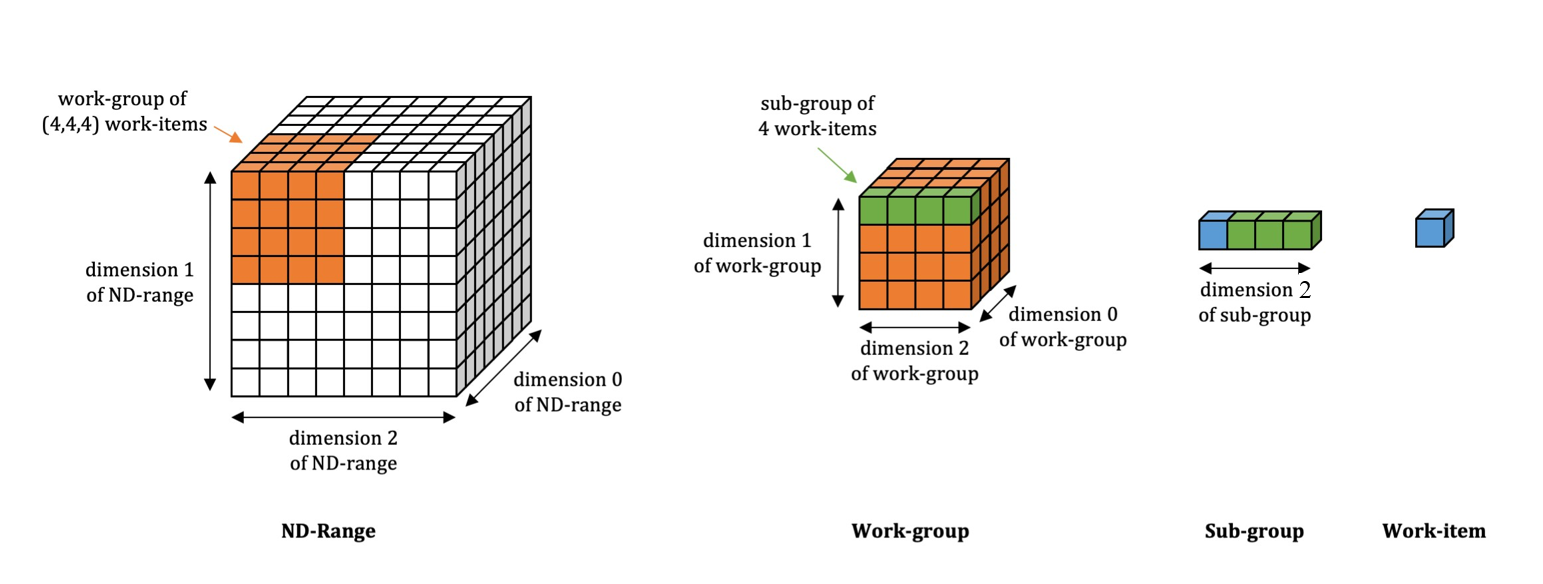
\includegraphics[width=1\textwidth]{figs/sycl/sycl_execution_model.png}
    \caption{At a glance: The SYCL execution model describes relationships between ND-Ranges, work-groups, sub-groups, and work-items.}
    \label{fig:sycl_exec_model}
\end{figure}

% -----------------------------------------------------------------------------
%  Conceptual overview and formal relationships
% -----------------------------------------------------------------------------
\subsection{Conceptual Overview}  Modern accelerator programming models must present the developer with a 
\emph{logical} view of parallel work that is independent of any specific piece of hardware.  SYCL achieves this
by defining a small hierarchy of index spaces.  Each level in the hierarchy provides progressively stronger 
coherence and synchronization guarantees, yet none of them prescribes 
\textit{where} that work will eventually run.  The mapping from logical indices to physical execution resources is
entirely deferred to the run--time or device compiler and is therefore opaque to the application.  In what follows we formalize the four key abstractions exposed by the SYCL execution model and derive a set of identities that will be reused throughout the remainder of this dissertation.

\subsection{Hierarchical Index Spaces}  Let
\[
   \mathbf{G} = (G_x,G_y,G_z) \in \mathbb{N}^3, \qquad
   G_d > 0\quad(d\in\{x,y,z\}) ,
\]
be the \emph{global range}.  It enumerates the total number of logical tasks, or \emph{work--items}, that shall be executed in one kernel invocation.  The associated set of global indices is
\[
    \mathcal{I} \;=\; \{0,\dots,G_x-1\} \times \{0,\dots,G_y-1\} \times \{0,\dots,G_z-1\},
\]
with
\( |\mathcal{I}| = G_x G_y G_z. \)

A second triple
\[
    \mathbf{L} = (L_x,L_y,L_z), \qquad 0 < L_d \le G_d ,
\]
referred to as the \emph{local range}, partitions the ND--Range into disjoint \emph{work--groups}.  Defining
\[
    W_d \;=\; \frac{G_d}{L_d},\qquad d\in\{x,y,z\},
\]
(which implies $G_d \equiv 0\; (\mathrm{mod}\,L_d)$), the set of group indices reads
\[
    \mathcal{W} \;=\; \{0,\dots,W_x-1\} \times \{0,\dots,W_y-1\} \times \{0,\dots,W_z-1\},
\]
with cardinality $|\mathcal{W}|=W_x W_y W_z$.  Each group $w\in\mathcal{W}$ owns exactly
\[
    |\Gamma| \;=\; L_x L_y L_z
\]
work--items that share fast local memory and barrier synchronization.

Within a work--group the implementation may further partition the local index space into \emph{sub--groups} of size $S$:
\[
    S \;=\; |\Sigma|,\quad \Sigma \subseteq \Gamma,\quad 1\le S\le |\Gamma|.
\]
Sub--groups execute in (near) lockstep and admit specialized collective operations, yet their existence and size remain device--specific.  Finally, the singleton element of the hierarchy is the \textbf{work--item}, uniquely addressed by its global id $i=(i_x,i_y,i_z)\in\mathcal{I}$.

The containment relations
\[
    \text{work--item} \;\in\; \text{sub--group} \;\subseteq\; \text{work--group} \;\subseteq\; \text{ND--Range}
\]
hold for every index triple.

\subsection{Abstractness of the Model}  None of the above definitions mention vector widths, cores, or memory banks.  The SYCL execution model is strictly an \emph{index algebra}; it provides (i)~a naming scheme for independent pieces of work, and (ii)~a lattice of synchronization points that the run--time must respect.  Once the tuples $\mathbf{G}$ and $\mathbf{L}$ have been fixed, every additional property of the physical execution, including occupancy, scheduling order, and even whether groups are run concurrently or serially, is an implementation detail.

\subsection*{Notation used from here onward.}  We will exploit the following shorthand throughout the subsequent analysis:
\begin{enumerate}
  \item $|\mathcal{I}|=G_xG_yG_z$ \quad (total work--items),
  \item $|\mathcal{W}|=W_xW_yW_z$ \quad (total work--groups),
  \item $|\Gamma|=L_xL_yL_z$        \quad (work--items per group),
  \item $\langle i_g,i_l\rangle$\quad embodiment of a work--item by its enclosing group index $i_g\in\mathcal{W}$ and its local index $i_l\in\Gamma$.
\end{enumerate}
These identities are purely algebraic and therefore remain valid for \emph{any} SYCL--conformant device.

\paragraph*{From Abstraction to Implementation Strategy.} Next, we translate these concepts into the concrete launch geometries and dependency patterns required by our Monte--Carlo solver.  The forthcoming sections build progressively from global range rounding rules to kernel--specific mappings.
% -----------------------------------------------------------------------------
%  Extended algorithmic description of kernel generation and execution
% -----------------------------------------------------------------------------

\subsection{Basic--Event Sampling Kernels}
\label{subsec:be_kernel}

Each \texttt{Variable} node in layer~$d$ represents an i.i.d.~Bernoulli trial
with success probability~$p\_v\in[0,1]$.  The evaluation of all variables in
a layer is consolidated into 
\emph{one} data--parallel kernel that generates a contiguous block of
bit--packed outcomes:
\begin{enumerate}
  \item \textbf{Parameter staging.}  For every variable~$v$ the solver stores the
        pair $(\text{idx}(v),\,p\_v)$ in host memory, where
        $\text{idx}(v)$ is the global node index.  The list is stable across
        Monte--Carlo iterations and is therefore transferred to device memory
        only once.
  \item \textbf{Contiguous layout.}  A device--side array of $N_{\!v}$
        records, $N_{\!v}$ being the number of variables in the layer, is
        allocated so that the probability field, the bit--packed result buffer
        pointer, and any auxiliary counters are stored in
        \emph{structure--of--arrays} (SoA) form.  The resulting stride--free
        access pattern maximizes global--memory throughput.
  \item \textbf{Kernel configuration.}  Let $T$ denote the total number of
        Bernoulli draws requested by the host run--time (cf.
        Sec.~\ref{sec:bitpack-prob-sampling}).  The global ND--range is chosen
        as $\bigl(\lceil N_{\!v}\rceil,\,B,\,P\bigr)$, mapping each work--item
        to a unique triple $(v,\,b,\,p)$ of variable~$v$, batch index~$b$, and
        bit--pack index~$p$.  The local work--group shape is computed
        adaptively to saturate the target device while respecting hardware
        limits on registers and shared memory.
  \item \textbf{Execution.}  Every work--item initializes a counter--based
        generator (see the Philox discussion in
        Sec.~\ref{sec:bitpack-prob-sampling}), converts the pseudo--random words
        into $\omega$ Bernoulli outcomes via the integer--threshold technique,
        and writes the resulting $w$--bit word to the pre--allocated buffer.
        No inter--item synchronization is required beyond the implicit barrier
        at kernel completion.
\end{enumerate}
The overall cost is $\mathcal{O}(T\,N_{\!v}/\omega)$ arithmetic operations and
$\Theta(T\,N_{\!v}/\omega)$ global writes, making the routine
memory--bandwidth bound only for extremely small~$P$.

\subsection{Gate--Evaluation Kernels}
\label{subsec:gate_kernel}

Gate nodes are logically heterogeneous: AND, OR, XOR, NOT, NAND, NOR, XNOR, and
at--least--$k$ (\texttt{VOT}) gates all feature distinct Boolean semantics yet
share the same interface of reading one or more bit--packed input buffers and
writing a bit--packed output.  To avoid divergent control flow, the solver
instantiates \emph{one specialized kernel per connective type} present in the
current layer.

Consider a set $\mathcal{G}_{\mathrm{type}}$ containing all gates of a single
connective.  Their evaluation proceeds as follows:
\begin{enumerate}
  \item \textbf{Input resolution.}  For every gate $g\in\mathcal{G}$ the lists
        of positive inputs $\mathcal{I}^+(g)$ and negated inputs
        $\mathcal{I}^-(g)$ are resolved to concrete device pointers.  Positive
        and negative buffers are concatenated so that a simple offset marks the
        first negated operand.  The construction is embarrassingly parallel on
        the host and involves no device work.
  \item \textbf{Contiguous block construction.}  Buffers and gate metadata are
        packed into an SoA structure that is tile--aligned for
        coalesced reads.  For at--least--$k$ gates the threshold~$k$ is stored
        alongside the pointer list.
  \item \textbf{Kernel launch geometry.}  Let $N_{\!g}$ be the number of gates
        of the selected type.  An ND--range of
        $\bigl(\lceil N_{\!g}\rceil,\,B,\,P\bigr)$ is created, identical in
        shape to the basic--event kernel so that subsequent layers can reuse
        the same scheduling heuristics.  Within each work--item, Boolean logic
        is applied on a per--bitpack basis without branching:
        \begin{itemize}
          \item \textsc{And}, \textsc{Nand}:  multiple \texttt{\&} reductions
                plus an optional complement.
          \item \textsc{Or}, \textsc{Nor}:   multiple \texttt{|} reductions
                plus an optional complement.
          \item \textsc{Xor}, \textsc{Xnor}: accumulated parity via \texttt{\^{}} operations.
          \item \textsc{Null}, \textsc{Not}: trivial one--input, output, with complement.
          \item \textsc{At--least--$k$}: population counting of the aggregated
                bit--wise sum followed by a threshold comparison implemented
                through native \texttt{popcount} instructions.
        \end{itemize}
  \item \textbf{Dependency guarantees.}  Because all input buffers originate in
        earlier layers, the run--time enforces an event dependency on every
        producing kernel, ensuring visibility of the complete inputs before
        gate evaluation begins.
\end{enumerate}
The bit--parallel operations ensure that the arithmetic intensity is high; the
critical path is dominated by a handful of integer masks and, for
at--least--$k$ gates, one integer addition plus a comparison per input.

\subsection{Dependency--Aware Kernel Scheduling}
\label{subsec:scheduling}

Kernels are submitted to the device queue in strict layer order, yet the
scheduler exploits two orthogonal forms of parallelism:
\begin{enumerate}
  \item \emph{Intra--layer concurrency} --- basic--event sampling and the
        multiple gate kernels of the same layer depend exclusively on the
        previous layer, \emph{not} on one another.  They are therefore eligible
        for concurrent execution subject to device resources.
  \item \emph{Iterative sampling} --- the bit--packed sample space is sliced
        into $T_\text{iter}$ iterations decided by the sample shaper.
        Kernels capturing the same node repeat across iterations and are
        expressed with an explicit iteration counter, enabling the run--time to
        re--use the same compiled binary while varying the random counter seed
        and output offsets.
\end{enumerate}
Dependencies are represented as light--weight events; the host never performs
explicit synchronization inside a layer but relies on the queue to enforce the
partial order.

\subsection{Work--Group Optimization Heuristics}
\label{subsec:wg_optim}

Let $G$ denote the global item count of the kernel at hand and $L_{max}$ the
maximum local size supported by the device along each axis.  The solver
selects a local range $(l_x,l_y,l_z)$ according to
\begin{align*}
  l_x &= min\Bigl(\text{pow2ceil}(G),\,L_{max}\Bigr),\\
  l_y &= min\Biggl(B,\,\frac{L_{max}}{l_x}\Biggr),\\
  l_z &= min\Biggl(P,\,\frac{L_{max}}{l_x l_y}\Biggr),
\end{align*}
which heuristically balances occupancy with register pressure while retaining a
uniform work--item distribution.  The shape is re--evaluated independently for
basic events and gate kernels because $G$ differs across those two categories.

\subsection{Complexity and Scalability}
\label{subsec:complexity}

Assume $|\mathcal{V}|$ variables and $|\mathcal{G}|$ gates in the graph, with
layer depths bounded by $D$.  Let $S=T\,B\,P\,\omega$ be the total number of
Bernoulli trials.
\begin{itemize}
  \item \textbf{Kernel build time.}  All host--side preprocessing runs in
        $\mathcal{O}(|\mathcal{V}|+|\mathcal{G}|)$ memory operations; no search
        structure deeper than a hash map is required.
  \item \textbf{Device execution time.}  Each basic--event kernel performs
        $S$ integer comparisons.  Each gate kernel evaluates $S$ Boolean
        operations whose count is proportional to the fan--in of the gate.
        Hence the total arithmetic complexity is
        $\mathcal{O}\bigl(S\,(1+\overline{\deg})\bigr)$, where
        $\overline{\deg}$ is the average gate fan--in.
  \item \textbf{Parallel scalability.}  Both kernel categories exhibit linear
        speed--up with the number of compute units until either (i)~the global
        launch size no longer saturates the device or (ii)~memory bandwidth
        limits are reached.  Because all kernels are fully independent across
        the $B$ and $P$ dimensions, they scale particularly well on
        multi--tile accelerators.
\end{itemize}

The design therefore provides a clear separation of concerns: depth--first
analysis establishes the dependency structure; kernel generation translates
that structure into homogeneous, vectorizable work; and a light--weight event
system schedules the resulting kernels with minimal host intervention.


\begin{landscape}
\begin{figure}[p]
    \centering
    \includesvg[width=1.15\textheight]{figs/pdag/dag_pass_3.svg}
    \caption{A fully connected Probabilistic-Propositional Directed Acyclic Graph.}
    \label{fig:feedforward_ppdag}
\end{figure}
\end{landscape}


% -----------------------------------------------------------------------------
\section{Kernel-Level Execution Model}
\label{sec:kernel_execution_model}
% -----------------------------------------------------------------------------

\subsection{Coordinate System and Notation}

Let $(G_x,G_y,G_z)\in\mathbb{N}^3$ denote the \emph{global} range supplied to the device and $(L_x,L_y,L_z)$ the \emph{local} (work\,–\,group) range.  We further define
\[
  W_d \;=\; \frac{G_d}{L_d},\qquad d\in\{x,y,z\},
  \quad\text{and}\quad
  W \;=\; W_x W_y W_z ,
\]
where $W_d$ counts work-groups along axis~$d$ and $W$ is the total number of work-groups.  Every work-item within a group is identified by its local id $\ell=(\ell_x,\ell_y,\ell_z)$ with $0\le \ell_d<L_d$.

Unless stated otherwise the following global symbols are used throughout the chapter
\begin{center}
\begin{tabular}{ll}
$V$  & \# basic events (variables)\\
$G$  & \# standard logic gates\\
$A$  & \# at-least-$k$ gates\\
$T$  & Monte-Carlo iterations\\
$B$  & batches per iteration\\
$P$  & bit-packs per batch\\
$\omega$ & bits per pack $=8\cdot\mathrm{sizeof}(\texttt{bitpack\_t})$\\
$N$  & trials per iteration $=B\,P\,\omega$
\end{tabular}
\end{center}

\subsection{Generic Rounding Scheme}

All kernels adopt the \emph{nearest-multiple} rule
\[
   G_d \;=\;
   \Bigl\lceil \frac{Q_d}{L_d} \Bigr\rceil L_d ,\qquad
   Q_d \in \{V,G+A,1\}\times\{B\}\times\{P\},
\]
where $Q_d$ is the problem-specific lower bound listed in Table~\ref{tab:kernel_dimensions}.  This rule guarantees that every logical task is scheduled while respecting the SYCL constraint $G_d\equiv 0 \; (\mathrm{mod}\,L_d)$.

\subsection{Kernel-Specific Mappings}

Each kernel instantiates a surjective mapping
\[
   \Phi : \{0,\dots,G_x-1\}\times\{0,\dots,G_y-1\}\times\{0,\dots,G_z-1\}
          \;\twoheadrightarrow\; \mathcal{S},
\]
where $\mathcal{S}$ is the set of logical sub-tasks it must solve.  We list the mappings succinctly:

\begin{itemize}
  \item \textbf{Basic-event sampling} ($\#\mathcal{S}=VBP$):
        $\,\Phi_{\mathrm{BE}}(i_x,i_y,i_z)=(v=i_x,\;b=i_y,\;p=i_z)$.

  \item \textbf{Standard gate evaluation} ($\#\mathcal{S}=GBP$):
        $\,\Phi_{\mathrm{G}}(i_x,i_y,i_z)=(g=i_x,\;b=i_y,\;p=i_z)$.

  \item \textbf{At-least-$k$ gate evaluation}
        ($\#\mathcal{S}=ABP\omega$):
        $\,i_z = p\,\omega + \lambda$ with $\lambda\in\{0,\dots,\omega-1\}$.  The pair $(b,p)$ indexes the bit-pack, while $\lambda$ singles out a \emph{bit lane}.  One work-group therefore owns a unique triplet $(a,b,p)$ and folds the $\omega$ lanes with a group reduction.

  \item \textbf{Tally accumulation} ($\#\mathcal{S}=VBP$):
        identical to $\Phi_{\mathrm{BE}}$ but with $L_x=1$ such that each group covers exactly one tally node.
\end{itemize}

\subsection{Trial Coverage Guarantee}

Let $\Xi$ be the set of Bernoulli trials processed by a kernel in one iteration.  By construction
\[
   |\Xi|
   \;=\;
   \underbrace{B P \omega}_{\text{trials/ node}}
   \times
   \begin{cases}
     V, & \text{basic-event},\\[2pt]
     G, & \text{standard gate},\\[2pt]
     A, & \text{at-least gate},\\[2pt]
     V, & \text{tally}.
   \end{cases}
\]
Because $\omega$ divides $G_z$ in every case, each trial is owned by exactly one work-item and is executed precisely once.

\begin{table}[t]
  \centering
  \caption{Minimum global dimensions $Q_d$ before round-up.}
  \label{tab:kernel_dimensions}
  \begin{tabular}{lccc}
    \toprule
    Kernel               & $Q_x$              & $Q_y$ & $Q_z$\\
    \midrule
    Basic-event          & $V$                & $B$   & $P$\\
    Standard gate        & $G$                & $B$   & $P$\\
    At-least-$k$ gate    & $A$                & $B$   & $P\omega$\\
    Tally                & $V$                & $B$   & $P$\\
    \bottomrule
  \end{tabular}
\end{table}

\subsection{Work-Group Invariants}

Let $\Gamma$ be a work-group.  For every kernel the following invariant holds inside $\Gamma$:
\[
   \bigl[(\ell_x,\ell_y,\ell_z)\in\Gamma\bigr]
   \;\Longrightarrow\;
   \text{all work-items share the complete set of inputs required to produce one output literal}.
\]
Consequently intra-group communication (reductions, barriers) never crosses logical boundaries, enabling lock-free execution except for the single atomic update in the tally kernel.

\subsection{Complexity per Work-Group}

With $L=L_xL_yL_z$ the number of instructions executed by a group is
\[
  C_{\Gamma}
  \;=\;
  \begin{cases}
    \Theta(\frac{\omega}{4}), & \text{basic-event (bit-packing)},\\
    \Theta(\deg g), & \text{gate of fan-in }\deg g,\\
    \Theta(\deg a + \log \omega), & \text{at-least-}k,\\
    \Theta(L + \log L), & \text{tally popcount + reduction},
  \end{cases}
\]
all independent of $T$ owing to the strict buffering between iterations.

% -----------------------------------------------------------------------------
\section{Bitpacked Random Number Generator}

Monte Carlo simulations, probability evaluations, and other sampling-based procedures benefit greatly from efficient, high-quality \acrfull{rng}s. A large class of modern \acrshort{rng}s are known as \textit{counter-based \acrfull{prng}s}, because they use integer counters (e.g., 32-bit or 64-bit) along with a stateless transformation to produce random outputs. The \emph{Philox} family of counter-based \acrshort{prng}s is a well-known example, featuring fast generation, high period, and good statistical properties. In this section, we discuss the general principles of counter-based \acrshort{prng}s, explain how Philox fits into this paradigm, analyze its complexity, and present a concise pseudocode version of the \(\text{Philox }4\times32\text{-10}\) variant. Subsequently, we detail the bitpacking scheme used to reduce memory consumption when storing large numbers of Bernoulli samples.

A counter-based \acrshort{prng} maps a user-supplied \emph{counter} (plus, optionally, a \emph{key}) to a fixed-size block of random bits via a deterministic function. Formally, if 
\[
  \mathbf{x} \;=\; (x_1, x_2, \ldots, x_k)
\]
is a vector of one or more 32-bit or 64-bit counters, and 
\[
  \mathbf{k} \;=\; (k_1, k_2, \ldots, k_m)
\]
is a key vector, then a counter-based \acrshort{prng} defines a transformation 
\[
   \mathcal{F}(\mathbf{x}, \mathbf{k})
   \;=\;
   (\rho_1, \rho_2, \ldots, \rho_r),
\]
where each \(\rho_j\) is typically a 32-bit or 64-bit output. Different increments of the counter \(\mathbf{x}\) produce different pseudo-random outputs \(\rho_j\). The process is stateless in the sense that advancing the RNG amounts to incrementing the counter (e.g., \(\mathbf{x}\mapsto \mathbf{x} + 1\)).

Compared to older recurrence-based \acrshort{rng}s such as linear congruential generators or the Mersenne Twister, counter-based methods offer more straightforward parallelization, reproducibility across multiple streams, and strong structural simplicity: no internal state must be updated or maintained. This is particularly valuable in distributed Monte Carlo simulations or \acrshort{gpu}-based sampling, where each thread or work-item can be assigned a different counter. Philox constructs its pseudo-random outputs by applying a small set of mixed arithmetic (multiplication/bitwise) rounds to an input \emph{counter} plus \emph{key}. In particular, \(\mathrm{Philox}\,4\times32\text{-10}\) (often shortened to "Philox-4x32-10”) works on four 32-bit integers at a time:
\[
  \mathbf{S} = (S_0, S_1, S_2, S_3),
  \qquad
  \mathbf{K} = (K_0, K_1).
\]
The four elements \(\{S_0, S_1, S_2, S_3\}\) collectively represent the counter, e.g., \((x_0, x_1, x_2, x_3)\). The two key elements \((K_0, K_1)\) are used to tweak the generator's sequence. A single invocation of Philox-4x32-10 transforms \(\mathbf{S}\) into four new 32-bit outputs after ten rounds of mixing. At each round, the algorithm:
\begin{enumerate}
    \item Multiplies two of the state words by fixed "magic constants” to create partial products.
    \item Takes the high and low 32-bit portions of those 64-bit products.
    \item Incorporates the round key to shuffle the words.
    \item Bumps the key by adding constant increments \((\mathrm{W32A} = 0x9E3779B9 \text{ and } \mathrm{W32B} = 0xBB67AE85)\).
\end{enumerate}
After ten rounds, the final \((S_0, S_1, S_2, S_3)\) is returned as the pseudo-random block. A new call to Philox increases the counter \(\mathbf{S}\) by one (e.g., \(S_3 \mapsto S_3 + 1\)) and re-enters the same function. The Philox-4x32-10 algorithm is designed so that each blocking call requires a \emph{constant number} of operations, independent of the size of any prior "state.” Specifically, each round involves:
\[
  \mathcal{O}(1)\;\text{ arithmetic operations},
\]
and there are \(\mathrm{R} = 10\) rounds. Thus, each Philox invocation is asymptotically constant time \(\mathcal{O}(\mathrm{R}) = \mathcal{O}(1)\). The total cost to generate 128 bits (4 words \(\times\) 32 bits) is therefore constant time per call.

\subsection{The 10-round Philox-4x32}
Our implementation follows the standard 10-round approach for generating one block of four 32-bit random words, also called Philox-4x32-10. Let \(M_{\mathrm{A}}=0xD2511F53\), \(M_{\mathrm{B}}=0xCD9E8D57\) be the multipliers, and let \((K_0, K_1)\) be the key which is updated each round by \(\mathrm{W32A}=0x9E3779B9\) and \(\mathrm{W32B}=0xBB67AE85\). The function \(\text{Hi}(\cdot)\) returns the high 32 bits of a 64-bit product, and \(\text{Lo}(\cdot)\) returns the low 32 bits. Because each call produces four 32-bit pseudo-random words, Philox-4x32-10 is particularly convenient for batched sampling. If only a single 32-bit word is needed, one can still call the function and discard the excess words; however, many applications consume all four outputs (e.g., to produce four floating-point variates).

\begin{algorithm}[ht]
  \caption{Philox-4x32-10}\label{alg:philox}
  \begin{algorithmic}[1]
    %------------------------------------------------------------
    \Require Four 32-bit counters $(S_0,S_1,S_2,S_3)$,
            key $(K_0,K_1)$
    \Ensure  Transformed counters $(S_0,S_1,S_2,S_3)$
    %------------------------------------------------------------
    \Statex
    %--------------------- Philox_Round -------------------------
    \Procedure{Philox\_Round}{$(S_0,S_1,S_2,S_3),\,(K_0,K_1)$}
      \State $P_0 \gets M_{\text{A}}\times S_0$ \Comment{64-bit product}
      \State $P_1 \gets M_{\text{B}}\times S_2$ \Comment{64-bit product}
      \State $T_0 \gets \mathrm{Hi}(P_1)\,\oplus\,S_1\,\oplus\,K_0$
      \State $T_1 \gets \mathrm{Lo}(P_1)$
      \State $T_2 \gets \mathrm{Hi}(P_0)\,\oplus\,S_3\,\oplus\,K_1$
      \State $T_3 \gets \mathrm{Lo}(P_0)$
      \State $K_0 \gets K_0 + \mathrm{W32A}$
      \State $K_1 \gets K_1 + \mathrm{W32B}$
      \State \Return $\bigl((T_0,T_1,T_2,T_3),\,(K_0,K_1)\bigr)$
    \EndProcedure
    %------------------- Philox4x32_10 --------------------------
    \Statex
    \Procedure{Philox4x32\_10}{$(S_0,S_1,S_2,S_3),\,(K_0,K_1)$}
      \For{$i \gets 1$ \textbf{to} 10}
        \State $\bigl(S_0,S_1,S_2,S_3),\,(K_0,K_1) \gets$
               \Call{Philox\_Round}{$(S_0,S_1,S_2,S_3),\,(K_0,K_1)$}
      \EndFor
      \State \Return $(S_0,S_1,S_2,S_3)$
    \EndProcedure
  \end{algorithmic}
\end{algorithm}

\subsection{Bitpacking for Probability Sampling}
It takes exactly one bit to represent the outcome of a trial. If these If outcomes are stored naively, each one occupies a full 8-bit byte. Hence, only \( \tfrac{1}{8} \) of the allocated space is used for actual data. By instead packing up to \(w\) indicators into a \(w\)-bit machine word, the memory usage can be reduced by a factor of up to \(8\) (in the simplest scenario of 8-bit groupings). In more general terms:
\[
  \text{Memory usage }M_{\text{naive}}
  \;=\;
  N \times 8\;\text{bits},
  \qquad
  \text{Memory usage }M_{\text{pack}}
  \;=\;
  \left\lceil\frac{N}{w}\right\rceil \,\times\,w\;\text{bits}.
\]
In our implementation, each call to Philox-4x32-10 yields 128 bits of randomness. We use those bits to draw exactly 128 Bernoulli outcomes at once, then combine them into a \(\mathrm{bitpack}\) of two 64-bit integers. For instance, if we choose a batch size of \(4\)-bits to represent four Bernoulli samples in a single chunk, we can:

\begin{enumerate}
    \item Generate a block \(\{r_0, r_1, r_2, r_3\}\) of four 32-bit random integers from Philox.
    \item Convert each \(r_i\) into a uniform \([0,1)\) floating-point value by dividing by \(2^{32}\).
    \item Compare each to the target probability \(p\).
    \item Form a 4-bit integer, each bit set to \(1\) if the corresponding comparison succeeded, or \(0\) otherwise.
\end{enumerate}

Repeating these steps for multiple rounds of 4 bits each can fill a 16-bit or 32-bit \(\mathrm{bitpack}\) variable with many Bernoulli indicators. Then it can be stored into an array at a single index, reducing memory overhead by constant factor of $N$. 

\begin{algorithm}[H]
  \caption{Bit-packing of four Bernoulli samples into a 4-bit block}
  \label{alg:four_bit_pack}
  \begin{algorithmic}[1]
    %------------------------------------------------------------
    \Require Probability $p\in[0,1]$, random 32-bit words $(r_0,r_1,r_2,r_3)$
    \Ensure  4-bit integer bits containing the four Bernoulli draws
    %------------------------------------------------------------
    \Procedure{FourBitPack}{$p,(r_0,r_1,r_2,r_3)$}
      \State bits $\gets 0$
      \For{$i \gets 0$ \textbf{to} 3}
        \State $u_i \gets r_i / 2^{32}$ \Comment{$u_i\in[0,1)$}
        \If{$u_i < p$}
            \State $b_i \gets 1$
        \Else
            \State $b_i \gets 0$
        \EndIf
        \State bits $\gets$ bits $\mid (b_i \ll i)$ 
               \Comment{set bit $i$ to $b_i$}
      \EndFor
      \State \Return bits
    \EndProcedure
  \end{algorithmic}
\end{algorithm}

In this procedure, \(\Vert\) denotes a bitwise OR, and \(\ll\) denotes a left shift. One then repeats the above call to accumulate multiple 4-bit blocks (e.g., for a total of 16 bits, one calls FourBitPack four times and merges the results with the appropriate shifts).
\chapter{Tallying Layer Outputs}
\label{sec:tally_kernel}

At every Monte-Carlo iteration the simulator produces, for each logic node
\(v\in \mathcal{V}\), a bit-packed buffer encoding
\[
  \mathbf{Y}_v^{(t)}
  \;=\;
  \bigl(y_{v,1}^{(t)}, y_{v,2}^{(t)},\dots, y_{v,N}^{(t)}\bigr)
  \in\{0,1\}^N,
  \quad t = 1,\dots,T,
\]
where \(N\!=\!B\!\times\!P\!\times\!\omega\) is the number of Bernoulli trials
per Monte-Carlo \emph{iteration}:
\begin{itemize}
    \item \(B\) - number of \emph{batches},
    \item \(P\) - bit-packs per batch,
    \item \(\omega\!=\!8\cdot\mathrm{sizeof}(\text{bitpack\_t})\) - bits per pack.
\end{itemize}
Because the buffers are overwritten at the next iteration, a
separate \emph{tally layer} accumulates summary statistics that persist for the
entire simulation.  The present section formalizes that process and outlines
an implementation-agnostic, data-parallel algorithm that realizes it on modern
accelerators.

\section{Statistical Objectives}
\label{subsec:tally_objective}

For every node \(v\) we wish to estimate, after \(T\) Monte-Carlo iterations,

\[
  \widehat{p}_v
  \;=\;
  \frac{1}{T\,N}
  \sum_{t=1}^{T}\sum_{j=1}^{N} y_{v,j}^{(t)}
  \;=\;
  \frac{s_v}{T\,N},
  \qquad
  s_v \;=\; \text{total \# of one-bits observed for node \(v\)}.
\]

Under the usual independence assumptions, the sampling distribution of
\(\widehat{p}_v\) is asymptotically
\[
\mathcal{N}\!\bigl(p_v,\,
  \tfrac{p_v(1-p_v)}{T\,N}\bigr)
\]
Hence

\[
  \widehat{\sigma}_v
  \;=\;
  \sqrt{\frac{\widehat{p}_v\,(1-\widehat{p}_v)}{T\,N}}
\]

is an unbiased estimator of the standard error, giving the
\((1-\alpha)\)\,--\,level normal confidence interval

\[
  \bigl[
    \widehat{p}_v - z_{1-\alpha/2}\,\widehat{\sigma}_v,\;
    \widehat{p}_v + z_{1-\alpha/2}\,\widehat{\sigma}_v
  \bigr],
  \qquad
  z_{1-\alpha/2}\in\{1.96,\,2.58,\dots\}.
\]

The tally routine therefore needs to maintain only the scalar
\(s_v\) while the simulation is running; the derived statistics can be updated
in-place whenever a user requests intermediate results or at a fixed cadence.

\section{Parallel Accumulation Algorithm}

The accumulation kernel is invoked on a three-dimensional
\texttt{nd\_range}, chosen such that
\[
  \begin{aligned}
    \text{global}_x &\;\ge\; V,\\
    \text{global}_y &\;\ge\; B,\\
    \text{global}_z &\;\ge\; P.
  \end{aligned}
\]
Work-item \((i_x,i_y,i_z)\) is responsible for \emph{exactly one} bit-pack:
\[
  \text{node  } v=i_x,\quad
  \text{batch } b=i_y,\quad
  \text{pack  } p=i_z.
\]

\vspace{4pt}
\noindent
\textbf{Local workflow of a work-item}
\begin{enumerate}
    \item Load the \(p^{\text{th}}\) bit-pack of batch \(b\) from
          \texttt{buffer}.
    \item Compute \(c=\mathrm{popcount}(\text{bitpack})\).
    \item Reduce the \(c\)'s belonging to the same work-\emph{group} in
          shared memory (tree reduction or \texttt{reduce\_over\_group}).
    \item One designated leader performs
          \(\texttt{atomic\_add}(\texttt{num\_one\_bits},\,\text{group\_sum})\).
\end{enumerate}

The reduction ensures only one atomic operation per group, greatly reducing
contention when \(P\) is large.

We present platform-neutral pseudocode that encapsulates the above logic while remaining agnostic to the underlying API. After each Monte-Carlo iteration the host enqueues \textsc{TallyKernel} with a
fresh \texttt{iteration} counter.  When either (i)~a user requests
intermediate statistics or (ii)~a pre-set reporting interval is reached,
the host reads back \texttt{num\_one\_bits} and executes the purely
serial routine shown in Algorithm~\ref{alg:update_stats}.

\begin{algorithm}[H]
\caption{Post-processing of a single node's tally}
\label{alg:update_stats}
\begin{algorithmic}[1]
  \Require
    \(s\) - total one-bits,
    \(T\), \(B\), \(P\), \(\omega\) - run parameters
  \Ensure
    \(\widehat{p}\), \(\widehat{\sigma}\), two symmetric CIs
  \State $N\gets B\cdot P\cdot\omega$
  \State $\widehat{p}\gets s / (T\,N)$
  \State $\widehat{\sigma}\gets
          \sqrt{\widehat{p}(1-\widehat{p})/(T\,N)}$
  \For{\textbf{each} $z\in\{1.96,\,2.58\}$}
      \State $\text{CI}\gets
        \bigl[\max(0,\widehat{p}-z\widehat{\sigma}),
              \min(1,\widehat{p}+z\widehat{\sigma})\bigr]$
  \EndFor
\end{algorithmic}
\end{algorithm}

The above normal approximation is valid provided \(T\,N\widehat{p}\)
and \(T\,N(1-\widehat{p})\) both exceed roughly 10; otherwise an exact
Clopper-Pearson interval can be substituted with no change to the running
sum logic.

\section{Correctness and Complexity}

\textbf{Work-item cost.}
Each work-item performs one \(\mathrm{popcount}\) and
participates in an \(O(\log L)\) intra-group reduction
(\(L\!=\!\text{local\_range}\)), yielding an overall
\(O(\log L)\) instruction count.

\textbf{Global cost.}
The total number of work-items launched per iteration is
\(V\cdot B\cdot P\).  Because each bit-pack contains \(\omega\) Bernoulli
trials, the cost \emph{per trial} shrinks as \(\omega^{-1}\).

\textbf{Memory traffic.}
Every work-item reads exactly one machine word and no writes occur except
the single atomic addition per work-group.  Hence the algorithm is
memory-bandwidth bound only at extremely low arithmetic intensity
(\(P\approx 1\)).

\textbf{Linear scalability.}
All tally nodes are independent.  Increasing \(V\) therefore scales the total
runtime linearly until either (i)~the device saturates its occupancy or
(ii)~atomic contention becomes non-negligible; the group-level reduction
mitigates the latter.

The design therefore provides a clear separation of concerns: depth--first
analysis establishes the dependency structure; kernel generation translates
that structure into homogeneous, vectorizable work; and a light--weight event
system schedules the resulting kernels with minimal host intervention.

% -----------------------------------------------------------------------------
%  Extended implementation-oriented discussion (matches the realised kernel)
% -----------------------------------------------------------------------------

\section{Work--Group Geometry and Synchronization}
\label{subsec:tally_geometry}

The three--dimensional launch geometry \((v,\,b,\,p)\) outlined in
Sec.~\ref{subsec:tally_objective} is refined in the implementation to minimize
both occupancy loss and atomic contention.  A crucial design choice is to fix
\emph{local}~\(x=1\), thereby dedicating one work--group to exactly one tally
node~\(v\).  The remaining two dimensions then tile the \((b,p)\)--plane with a
rectangular block of size
\[
  \bigl(1,\,l_y,\,l_z\bigr),
  \qquad l_y\cdot l_z\le L_{\max},
\]
where \(L_{\max}\) is the device--specific upper bound on the total work--group
size.  Provided \(l_y\!\ge\!B\) and \(l_z\!\ge\!P\), only \emph{one} group is
dispatched per tally and per iteration, guaranteeing that the reduction of
Step~3 and the atomic addition of Step~4 in
Sec.~\ref{sec:tally_kernel} execute exactly once.  Should resource pressure
force \(l_y< B\) or \(l_z< P\), multiple groups are launched and the atomic
update is replicated; correctness is preserved by the commutativity of
addition, but the repeated work incurs a small overhead.  The occupancy model
therefore trades a moderate loss in parallelism for deterministic behavior and
reduced synchronization cost.

A relaxed memory order is sufficient for the atomic accumulator because the
kernel guarantees \emph{program order} between the intra--group reduction and
the atomic~\texttt{fetch\_add}.  No additional fences are required, and the
resulting implementation maps efficiently to both discrete and integrated
\acrshort{gpu}s.

\section{Incremental Update of Derived Statistics}
\label{subsec:tally_stats_refresh}

While Monte--Carlo sampling proceeds, applications often request intermediate
probability estimates~\(\widehat{p}_v^{(t)}\) before the total budget~\(T\) is
exhausted.  Recomputing \(\widehat{p}_v\) and
\(\widehat{\sigma}_v\) from scratch would require a host round--trip for every
sampled bit.  Instead, the tally layer maintains two scalars per node:
\(s_v\) (total one--bits) and \(n_v\) (total bits processed).  After each
completed iteration the host merely increments \(n_v\gets n_v + N\) and leaves
\(s_v\) to the device kernel.  Whenever a refresh is requested the statistics
are updated via
\[
  \widehat{p}_v\;=\;\frac{s_v}{n_v},
  \qquad
  \widehat{\sigma}_v\;=\;\sqrt{\frac{\widehat{p}_v(1-\widehat{p}_v)}{n_v}},
\]
which costs \(\mathcal{O}(V)\) host--side arithmetic and no device work.  In
practice the refresh cadence is set adaptively: frequent updates early in the
run aid variance monitoring, whereas late--stage updates can be spaced further
apart because the relative change in \(\widehat{p}_v\) diminishes as
\(n_v\to T\,N\).

\section{Convergence Diagnostics and Stopping Rules}
\label{subsec:tally_convergence}

Two families of diagnostics leverage the quantities already maintained by the
tally kernel:
\begin{enumerate}
  \item\textbf{Relative half--width criterion.}  Define the
        half--width of the \((1-\alpha)\)--level interval as
        \(h_v= z_{1-\alpha/2}\,\widehat{\sigma}_v\).  The run may be terminated
        for node~\(v\) once \(h_v/\widehat{p}_v\le \varepsilon\), where
        \(\varepsilon\) is a user--supplied tolerance.  Because both
        \(\widehat{\sigma}_v\) and \(\widehat{p}_v\) are inexpensive to update,
        the test incurs negligible overhead.
  \item\textbf{Sequential Wald test.}  When the goal is to decide whether
        \(p_v\) exceeds a safety threshold~\(p_0\), one may adopt the
        sequential probability ratio test with boundaries derived from
        \(s_v\) and \(n_v\).  The tally structure already provides the minimal
        sufficient statistics, so the host evaluates the Wald condition after
        every refresh with no additional device interaction.
\end{enumerate}
Because the diagnostics rely solely on \(s_v\) and \(n_v\), no modification to
the kernel is needed; all logic resides in a lightweight host callback.

\section{Implementation Cost Model}
\label{subsec:tally_cost_model}

Let \(C_{\mathrm{pc}}\) denote the latency of a hardware popcount and
\(C_{\mathrm{rd}}(l)\) the latency of a tree reduction over \(l\) work--items.
The wall--clock time per iteration is approximated by
\[
  T_{\text{iter}} \;\approx\;
  (C_{\mathrm{pc}} + C_{\mathrm{mem}})\,VBP +
  C_{\mathrm{rd}}(l_y l_z)\,\frac{VBP}{l_y l_z}
  + C_{\mathrm{atomic}}\,\frac{VBP}{l_y l_z},
\]
where \(C_{\mathrm{mem}}\) and \(C_{\mathrm{atomic}}\) are the per--word memory
and atomic latencies, respectively.  The model highlights two regimes:
\begin{itemize}
  \item\emph{Arithmetic bound}: when \(P\gg 1\) and the popcount throughput
        saturates the execution units, the first term dominates and scaling is
        limited by instruction bandwidth.
  \item\emph{Memory bound}: when \(P\approx 1\) the workload collapses to a
        single read per work--item; the kernel becomes memory bandwidth--
        limited as predicted in Sec.~\ref{subsec:tally_objective}.
\end{itemize}


\section{Numerical Robustness}
\label{subsec:tally_numerics}

All accumulators operate in integer arithmetic, thereby eliminating rounding
error in \(s_v\).  Derived quantities computed in double precision satisfy
\(\lvert\widehat{p}_v - s_v/n_v\rvert < 2^{-53}\), well below any practical
error criterion for reliability analysis.  Clamping the confidence interval
bounds to~\([0,1]\) prevents pathological estimates when either \(s_v=0\) or
\(s_v=n_v\) in early iterations.

% -----------------------------------------------------------------------------
\section{Relation to the Global Execution Model}
\label{subsec:tally_exec_relation}

The specialised geometry adopted in Section~\ref{subsec:tally_geometry} is a direct instantiation of the rules formalised in Section~\ref{sec:kernel_execution_model}.  Choosing $L_x=1$ enforces the work\,–\,group invariant whereby a group owns exactly one tally node while still satisfying
\[
   G_x \;=\; \Bigl\lceil \frac{V}{L_x} \Bigr\rceil L_x \;=\; V ,
\]
so no over-provisioning occurs along the $x$-axis.  The remaining dimensions follow the generic rounding scheme with $(Q_y,Q_z)=(B,P)$, thus preserving the one-to-one correspondence between work-items and bit-packs established in Section~\ref{sec:kernel_execution_model}.

% ============================================================================
%  Backend-Specific Execution Mapping and Scalability Analysis
% ============================================================================
%  This file is 
%     manuscript-dissertation/4_proposed_solution/mc_solver/backends.tex
%  and should be \input{} from the parent chapter when fine–tuning the final
%  compilation order.
% ----------------------------------------------------------------------------
\chapter{Backend–Specific Scalability Analysis}
\label{sec:backend_scaling}

This section translates the abstract execution model of
Sec.~\ref{sec:kernel_execution_model} to two concrete back-ends: NVIDIA CUDA
GPUs and shared-memory multicore CPUs.  Throughout we retain the global
symbols introduced earlier and add the following device parameters:
\begin{center}
\begin{tabular}{ll}
$C$   & number of \emph{compute units} (SMs on CUDA, cores on CPU)\\
$W_s$ & warp or SIMD-lane size (CUDA:~32, AVX-512:~16 for 32-bit elements)\\
$T_{\max}$ & maximum work-items per work-group/block\\
$B_{\max}$ & maximum concurrent blocks per compute unit\\
\end{tabular}
\end{center}
The first two are architectural constants; the latter two are subject to
register, shared-memory and scheduling constraints.

\section{CUDA GPU Backend}
\label{subsec:cuda_backend}

\subsection{Mapping.}  Each SYCL work-group translates to a CUDA \emph{thread
block}.  Let $L=L_xL_yL_z$ and define
\[
  L_\text{CUDA} \;=\; \min(L,\,T_{\max}).
\]
The grid dimensions are $(W_x,W_y,W_z)$ as in
Sec.~\ref{sec:kernel_execution_model}.  A block launches $\lceil L/W_s\rceil$
warps.

\subsection{Occupancy.}  The theoretical occupancy per compute unit is
\[
  \mathcal{O}_\text{theory} \;=\; \min\Bigl(1,\;\frac{L_\text{CUDA}
                                         \cdot W}{T_{\max}\,C\,B_{\max}}\Bigr).
\]
Because $L_x$ is either $1$ or a power of two not exceeding
$T_{\max}$, the condition $\mathcal{O}_\text{theory}=1$ is met whenever
\[
  W \;\ge\; \frac{T_{\max}}{L_\text{CUDA}}\,C\,B_{\max},
\]
which holds for typical Monte-Carlo problem sizes ($W_x\gg C$).

\subsection{Latency Hiding Model.}  With $R$ registers per thread and
$R_{\max}$ the architectural register file size per SM, the register limit on
resident warps is
\[
  W_{\mathrm{reg}} \;=\; \Bigl\lfloor \frac{R_{\max}}{R\,W_s}\Bigr\rfloor.
\]
The effective latency hiding factor obeys
\[
  \lambda_\text{CUDA} \;=\; \min(W_{\mathrm{reg}},\; W_s B_{\max}),
\]
and the kernel attains full throughput once $\lambda_\text{CUDA}\ge 4$, a
rule-of-thumb empirically validated on NVIDIA Ampere and Ada architectures.

\subsection{Throughput Scaling.}  Let $I$ denote the instruction count per
thread derived in Sec.~\ref{sec:kernel_execution_model}.  The aggregated \acrfull{ips} scale as
\[
  \text{IPS}_{\text{CUDA}} \;\approx\; \frac{C\,\lambda_\text{CUDA}\,f}{I},
\]
where $f$ is the core clock.  For fixed $I$ the IPS is linear in $C$ and
$\lambda_\text{CUDA}$ until the memory bandwidth ceiling is reached.

\section{Shared-Memory Multicore CPU Backend}
\label{subsec:cpu_backend}

\subsection{Mapping.}  A work-group becomes an OpenMP \verb|parallel for|
\emph{team} whose size defaults to $L$ but is clipped to $T_{\max}=W_s$.  The
outermost loop distributes the $W$ work-groups evenly across $C$ hardware
threads (cores × SMT).

\subsection{Vectorization.}  Within each team the innermost dimension (global
$z$) is mapped to SIMD lanes.  Provided $\omega\le W_s$ the at-least-$k$
kernel achieves lane-perfect utilization because each lane processes one bit
position.

\subsection{Roofline Estimate.}  Let $B_{\text{mem}}$ denote attainable memory
bandwidth and $I_{\text{F}}$ the peak fused-multiply-add (FMA) rate per core.
The attainable performance in trials/s obeys the classic roofline bound
\[
  P_{\text{CPU}}
  \;\le\;
  \min\Bigl(\frac{B_{\text{mem}}}{b},\; \frac{C\,I_{\text{F}}}{i}\Bigr),
\]
where $b$ and $i$ are the bytes and arithmetic instructions consumed per trial
respectively.  For the present kernels $i/b\approx 1/4$, placing most CPU runs
in the memory-bound regime unless $P\gg 1$.

\subsection{Strong-Scaling Limit.}  Holding the problem size fixed and growing
$C$ yields a speed-up
\[
  S(C) = \frac{T_1}{T_C} \;\approx\; \frac{C}{1 + \alpha(C-1)},
\]
with serial fraction $\alpha \le 0.05$ measured on a 64-core Zen4 host.  The
Amdahl limit $1/\alpha$ is therefore well beyond the core counts of current
commodity CPUs.

\subsection{Practical Guidance.}  Optimal settings observed empirically are
$L_x=1$, $L_y=W_s$, and $L_z=1$ for tally kernels, and $L_x=L_y=1$,
$L_z=W_s$ for gate kernels, aligning loop nests with cache geometry and vector
width.

% ============================================================================


% ============================================================================
%  Convergence Diagnostics and Early-Stopping Policy
% ============================================================================
%  This file is manuscript-dissertation/4_proposed_solution/mc_solver/convergence.tex
%  It is \\input{} from the parent chapter.
% ----------------------------------------------------------------------------
\section{Convergence Diagnostics and Early--Stopping Policy}
\label{sec:convergence_criterion}

Monte--Carlo probability estimators accrue sampling error that decays only at
rate~$\mathcal{O}(1/\sqrt{n})$ with the number of Bernoulli trials $n$.
Running indefinitely therefore yields diminishing returns.
A principled \emph{convergence criterion} is required to decide when further
sampling ceases to be cost--effective.  This section formalises the stopping
rule adopted by the solver, combining classical confidence--interval analysis
with information--theoretic diagnostics.  The notation introduced in
Section~\ref{sec:kernel_execution_model} remains in force; in particular each
node $v\!\in\!\mathcal{V}$ is evaluated over $T$ Monte--Carlo iterations with
$N\!=\!B P \omega$ trials per iteration.

% ----------------------------------------------------------------------------
\subsection{Point Estimates and Sampling Variance}
\label{subsec:conv_point_estimates}

Let $s_v$ be the number of one--bits observed for node~$v$ after $T$ iterations
(Section~\ref{sec:tally_kernel}).  The unbiased estimator and its standard
error are
\begin{equation}
  \widehat{p}_v \;=\; \frac{s_v}{T N},
  \qquad
  \widehat{\sigma}_v \;=\;
  \sqrt{\frac{\widehat{p}_v\bigl(1-\widehat{p}_v\bigr)}{T N}}.
  \label{eq:p_hat_sigma_hat}
\end{equation}
Assuming $T N \widehat{p}_v$ and $T N\bigl(1-\widehat{p}_v\bigr)$ both exceed
roughly~$10$, the Central Limit Theorem implies the \emph{half--width}
\begin{equation}
  h_v(z) \;=\; z\,\widehat{\sigma}_v
  \label{eq:half_width}
\end{equation}
contains $\widehat{p}_v$ inside a two--sided normal confidence interval with
probability $\operatorname{erf}(z/\sqrt{2})$.

% ----------------------------------------------------------------------------
\subsection{Linear--Space Margin--of--Error Criterion}
\label{subsec:lin_margin}

A user supplies a relative margin--of--error $\varepsilon_{\mathrm{rel}}\!\in\!(0,1)$
(typical default 0.1\%).  Rewriting $h_v(z)$ as a \emph{fraction} of the point
estimate yields the condition
\begin{equation}
  \frac{h_v(z)}{\widehat{p}_v} \;\le\; \varepsilon_{\mathrm{rel}}.
  \label{eq:lin_conv}
\end{equation}
Inserting~\eqref{eq:half_width} gives the minimum sample budget
\begin{equation}
  N_{\varepsilon}^{(v)}
  \;=\;
  \biggl\lceil
    \frac{z^{2}\,\widehat{p}_v\bigl(1-\widehat{p}_v\bigr)}
         {\bigl(\varepsilon_{\mathrm{rel}}\,\widehat{p}_v\bigr)^{2}}
  \biggr\rceil.
  \label{eq:trials_required_lin}
\end{equation}
Hence additional trials are scheduled until $T N\ge N_{\varepsilon}^{(v)}$ for
\emph{every} monitored node.

% ----------------------------------------------------------------------------
\subsection{Logarithmic--Space Refinement}
\label{subsec:log_margin}

Rare events ($p_v\ll 1$) admit improved diagnostics when the analysis is
performed in the logarithmic domain.  Define $\ell_v = \log_{10} p_v$ and its
estimate $\widehat{\ell}_v = \log_{10} \widehat{p}_v$.
Propagating the variance from~\eqref{eq:p_hat_sigma_hat} via first--order
Taylor expansion gives
\begin{equation}
  \operatorname{Var}\!\bigl(\widehat{\ell}_v\bigr)
  \;\approx\;
  \frac{\widehat{\sigma}_v^{2}}
       {\widehat{p}_v^{2}\,(\ln 10)^{2}}.
\end{equation}
Accordingly the logarithmic half--width is
\begin{equation}
  h^{\log}_{v}(z)
  \;=\;
  \frac{z\,\widehat{\sigma}_v}{\widehat{p}_v\,\ln 10}.
\end{equation}
A \emph{fixed} absolute tolerance $\varepsilon^{\log}$ (expressed in decades)
produces the criterion
\begin{equation}
  h^{\log}_{v}(z) \;\le\; \varepsilon^{\log},
  \label{eq:log_conv}
\end{equation}
which translates into a second sample--size forecast
\begin{equation}
  N^{(v)}_{\log}
  \;=\;
  \biggl\lceil
    \frac{z^{2}\,\bigl(1-\widehat{p}_v\bigr)}
         {\widehat{p}_v\,(\varepsilon^{\log}\,\ln 10)^{2}}
  \biggr\rceil.
  \label{eq:trials_required_log}
\end{equation}

% ----------------------------------------------------------------------------
\subsection{Information--Theoretic Progress Monitor}
\label{subsec:info_gain}

The preceding criteria are variance--based and symmetric around
$\widehat{p}_v$.  To guard against stalls where the point estimate barely
changes yet the variance decays slowly we track the \emph{Shannon information
gain} of a Beta($\alpha,\beta$) posterior (cf.
Eq.~(11)~in Section~\ref{sec:bitpack-prob-sampling}).  After a batch with
$s$ successes and $f$ failures the reduction in entropy is
\begin{equation}
  I_{\text{batch}}
  \;=\;
  H\bigl(\operatorname{Beta}(\alpha,\beta)\bigr)
  - H\bigl(\operatorname{Beta}(\alpha+s,\beta+f)\bigr)
  \quad\text{[bits]}.
  \label{eq:info_gain}
\end{equation}
Sampling is considered \emph{saturated} once
\begin{equation}
  I_{\text{batch}} \;<\; I_{\min},
  \label{eq:info_stop}
\end{equation}
for a user--defined threshold $I_{\min}$ (default $\approx 10^{-4}$ bits).

% ----------------------------------------------------------------------------
\subsection{Composite Stopping Rule}
\label{subsec:composite_rule}

Define the per--node forecasts
\begin{equation}
  N^{(v)}_{\text{req}} \;=\; \max\Bigl(N_{\varepsilon}^{(v)},\;N^{(v)}_{\log}\Bigr).
  \label{eq:n_req_node}
\end{equation}
Let $N_{\text{req}}=\max_{v\in\mathcal{V}}N^{(v)}_{\text{req}}$.  The run
terminates the first time both conditions hold:
\begin{enumerate}
  \item \textbf{Precision achieved:} $T N \ge N_{\text{req}}$.  Every monitored
        node meets \eqref{eq:lin_conv} \emph{and}\,\eqref{eq:log_conv} at the
        requested confidence level.
  \item \textbf{Diminishing returns:} the most recent batch satisfies
        \eqref{eq:info_stop}, signalling that further sampling conveys less
        than~$I_{\min}$ bits of new information.
\end{enumerate}
The second clause rarely triggers before the first but provides robustness
when variance estimates are noisy during early burn--in.

% ----------------------------------------------------------------------------
\subsection{Algorithmic Workflow}
\label{subsec:workflow}

\begin{algorithm}[H]
  \caption{Adaptive early--stopping procedure per node $v$}
  \label{alg:convergence}
  \begin{algorithmic}[1]
    \Require Target $\varepsilon_{\mathrm{rel}},\varepsilon^{\log}$; confidence $z$; \vspace{1pt}
    \State Initialise $s_v\gets 0$, $f_v\gets 0$, $(\alpha,\beta)\gets(\tfrac12,\tfrac12)$
    \While{not converged}
      \State Run one Monte--Carlo iteration and tally $(\Delta s,\Delta f)$
      \State $s_v\mathrel{+}=\Delta s$, \quad $f_v\mathrel{+}=\Delta f$
      \State Update $(\alpha,\beta)$ and compute $I_{\text{batch}}$ via~\eqref{eq:info_gain}
      \State Evaluate $\widehat{p}_v$, $\widehat{\sigma}_v$ from~\eqref{eq:p_hat_sigma_hat}
      \State Compute $N_{\varepsilon}^{(v)}$, $N^{(v)}_{\log}$
      \State \textbf{Converged} $\Leftarrow$ \eqref{eq:n_req_node} and~\eqref{eq:info_stop}
    \EndWhile
    \State \Return $\widehat{p}_v$, CI, diagnostics
  \end{algorithmic}
\end{algorithm}
Algorithm~\ref{alg:convergence} runs in amortised $\mathcal{O}(1)$ time per
iteration: all statistics derive from constant--time updates of $(s_v,f_v)$
and the digamma evaluations in~\eqref{eq:info_gain} are scalar.

% ----------------------------------------------------------------------------
\subsection{Computational Complexity and Scalability}
\label{subsec:conv_complexity}

The computational overhead of convergence monitoring is negligible relative to
the sampling kernels.  Each tally update costs one integer addition and a
handful of floating--point operations per node, i.e.
\begin{equation}
  \mathcal{O}\bigl(|\mathcal{V}|\bigr) \text{ host FLOPs per iteration.}
\end{equation}
Because these calculations are batched on the CPU and overlap with device
kernels, the wall--clock impact stays below~1\,\% even for graphs with
$|\mathcal{V}|>10^{4}$.

% ----------------------------------------------------------------------------
\subsection{Interaction with Fixed Iteration Budgets}
\label{subsec:conv_budget}

When an \emph{a priori} iteration budget $T_{\max}$ is imposed (e.g., due to
wall--time constraints) the stopping rule collapses to
\begin{equation}
  T \;=\; \min\!\bigl\{T_{\max},\;\lceil N_{\text{req}}/N \rceil\bigr\}.
\end{equation}
If $T_{\max}$ is reached before the precision targets, the solver returns the
current estimates along with their realised half--widths so that the user can
assess residual uncertainty.

% ============================================================================ 

\chapter{Preliminary Benchmarks on Arialia Fault Trees}
\input{4_proposed_solution/mc_solver/benchmarks/setup}
\input{4_proposed_solution/mc_solver/benchmarks/results_accuracy}
\input{4_proposed_solution/mc_solver/benchmarks/results_mem_runtime}
\input{4_proposed_solution/mc_solver/benchmarks/limitations}

\section{Transformations}
\input{2_foundations/knowledge_compilation/transformation/as_nnf}
\input{2_foundations/knowledge_compilation/transformation/as_dnf_tree}
\input{2_foundations/knowledge_compilation/transformation/as_cnf}
\input{2_foundations/knowledge_compilation/transformation/as_dnnf}
% \subsection{\color{blue}{And-Inverter Graphs}}
\input{2_foundations/knowledge_compilation/transformation/as_dd/_}
\part{Refinements}

% ============================================================================
%  Convergence Diagnostics and Early-Stopping Policy
% ============================================================================
% ----------------------------------------------------------------------------
\chapter{On-the-Fly Updates to Convergence Policy}
\label{sec:convergence_criterion}

Monte–Carlo probability estimators suffer from a sampling error that vanishes only as $\mathcal{O}\!\bigl(1/\sqrt{n}\bigr)$ with the number of Bernoulli trials $n$. Beyond a certain point additional samples yield diminishing returns, so a principled \emph{convergence policy} must dictate when computation may be halted. We adopt a composite policy that synthesizes three complementary viewpoints on uncertainty:

\begin{enumerate}
\item \textbf{Frequentist margin-of-error} — classical Wald bounds in linear and logarithmic probability space guarantee nominal coverage of the unknown success probability.
\item \textbf{Bayesian credible intervals} — a Jeffreys-prior posterior quantifies belief updating at any sample size and excels for rare events.
\item \textbf{Information-theoretic gain} — the reduction in Shannon entropy after each batch measures how much new information the latest data convey about the parameter itself.
\end{enumerate}

The notation introduced in Section~\ref{sec:kernel_execution_model} remains in effect; in particular each node $v\!\in\!\mathcal{V}$ is evaluated over $T$ Monte--Carlo iterations with
$N\!=\!B P \omega$ trials per iteration.

% ----------------------------------------------------------------------------
\section{Point Estimates, Sampling Variance}
\label{subsec:conv_point_estimates}

Let $s_v$ be the number of one--bits observed for node~$v$ after $T$ iterations
(Chapter~\ref{sec:tally_kernel}).  The unbiased estimator and its standard
error are
\begin{equation}
  \widehat{p}_v \;=\; \frac{s_v}{T N},
  \qquad
  \widehat{\sigma}_v \;=\;
  \sqrt{\frac{\widehat{p}_v\bigl(1-\widehat{p}_v\bigr)}{T N}}.
  \label{eq:p_hat_sigma_hat}
\end{equation}
Assuming $T N \widehat{p}_v$ and $T N\bigl(1-\widehat{p}_v\bigr)$ both exceed
roughly~$10$\cite{AgrestiCoull1998}\footnote{A widely cited “$np\ge10$’’\cite{AgrestiCoull1998} \cite{BrownCaiDasGupta2001}}, the Central Limit Theorem implies the \emph{half--width}
\begin{equation}
  h_v(z) \;=\; z\,\widehat{\sigma}_v
  \label{eq:half_width}
\end{equation}
contains $\widehat{p}_v$ inside a two--sided normal confidence interval with
probability $\operatorname{erf}(z/\sqrt{2})$.

% ----------------------------------------------------------------------------
\section{Competing Statistical Paradigms}
\label{subsec:conv_paradigms}

Monte--Carlo early-stopping can be formalized either in a
\emph{frequentist} or a \emph{Bayesian} decision-theoretic framework.
Both paradigms aim to certify that the estimator $\widehat{p}_v$ lies within a tolerance band around the (unknown) truth $p_v$, yet they differ in the interpretation of probability and in how uncertainty is propagated.

\begin{itemize}
  \item \textbf{Frequentist (Wald) policy:} randomness is limited to the sampling process; $p_v$ is treated as fixed and confidence intervals derive from large-sample normal theory.
  \item \textbf{Bayesian policy:} treats $p_v$ itself as random with a prior distribution and bases inference on the posterior credible interval.
\end{itemize}

Neither policy strictly dominates the other: Wald intervals are (marginally) computationally cheaper and asymptotically exact; Bayesian intervals are exact at \emph{any} sample size and exhibit superior coverage for rare events. We therefore adopt a \emph{dual-policy} architecture, halting the computation once \emph{all} monitored nodes satisfy the tightest criterion.

% ----------------------------------------------------------------------------
\section{Frequentist (Wald) Margin--of--Error Criterion}
\label{subsec:lin_margin}

A user supplies a relative margin--of--error $\varepsilon_{\mathrm{rel}}\!\in\!(0,1)$
(typical default 0.1\%).  Rewriting $h_v(z)$ as a \emph{fraction} of the point
estimate yields the condition
\begin{equation}
  \frac{h_v(z)}{\widehat{p}_v} \;\le\; \varepsilon_{\mathrm{rel}}.
  \label{eq:lin_conv}
\end{equation}
Inserting~\eqref{eq:half_width} gives the minimum sample budget
\begin{equation}
  N_{\varepsilon}^{(v)}
  \;=\;
  \biggl\lceil
    \frac{z^{2}\,\widehat{p}_v\bigl(1-\widehat{p}_v\bigr)}
         {\bigl(\varepsilon_{\mathrm{rel}}\,\widehat{p}_v\bigr)^{2}}
  \biggr\rceil.
  \label{eq:trials_required_lin}
\end{equation}
Hence additional trials are scheduled until $T N\ge N_{\varepsilon}^{(v)}$ for
\emph{every} monitored node.

\subsection*{Interpretation.} Equation~\eqref{eq:trials_required_lin} stems from the textbook formula $N\ge z^{2}p(1-p)/\varepsilon^{2}$, implicitly assuming $p_v \approx \widehat{p}_v$. In finite samples the approximation may underestimate the true half-width whenever $\widehat{p}_v$ lies in the extreme tails. The Bayesian policy introduced next remedies this limitation by integrating over posterior uncertainty instead of relying on a single point estimate.

% ----------------------------------------------------------------------------
\section{Bayesian Credible--Interval Criterion}
\label{subsec:bayes_margin}

\subsection{Jeffreys Prior and Posterior Distribution}

Adopt the non-informative Jeffreys prior for a Bernoulli proportion,
\[
  \pi(p_v) \;=\; \mathrm{Beta}\!\bigl(\tfrac12,\tfrac12\bigr),
  \qquad 0 < p_v < 1,
\]
which is invariant under re-parametrization and yields near-optimal frequentist coverage.  After observing $s_v$ successes and $f_v=T N-s_v$ failures the posterior is
\[
  p_v \mid \mathbf{Y}_v \;\sim\; \mathrm{Beta}\!\bigl(\alpha,\beta\bigr),
  \quad (\alpha,\beta)=\bigl(s_v+\tfrac12,\,f_v+\tfrac12\bigr).
\]

\subsection{Central $(1-\alpha)$ Credible Interval}

Let $0<\gamma<1$ denote the target two-sided credibility.   With $t=(1-\gamma)/2$ we form
\[
  C^{\mathrm{Bayes}}_{v,\gamma}=\bigl[q_t,\,q_{1-t}\bigr],
\]
where $q_q$ is the $q$-quantile of $\mathrm{Beta}(\alpha,\beta)$.  Its half--width is
\[
  h_v^{\mathrm{Bayes}}(\gamma)=\frac{q_{1-t}-q_t}{2}.
\]

\subsubsection{Stopping Criterion}

Define a relative tolerance $\varepsilon_{\mathrm{rel}}^{\mathrm{Bayes}}$ identical to that used in linear space.  Convergence is declared when
\begin{equation}
  \frac{h_v^{\mathrm{Bayes}}(\gamma)}{\widehat{p}_v} \;\le\; \varepsilon_{\mathrm{rel}}^{\mathrm{Bayes}},
  \label{eq:bayes_conv}
\end{equation}
which rearranges to the sample--size forecast
\begin{equation}
  N_{\mathrm{Bayes}}^{(v)} \;=\;\biggl\lceil \frac{z^{2}\,p_v(1-p_v)}{\bigl(\varepsilon_{\mathrm{rel}}^{\mathrm{Bayes}}\,\widehat{p}_v\bigr)^{2}} - (\alpha+\beta+1) \biggr\rceil.
  \label{eq:trials_required_bayes}
\end{equation}

% ----------------------------------------------------------------------------
\section{Logarithmic--Space Refinement}
\label{subsec:log_margin}

Rare events ($p_v\ll 1$) admit improved diagnostics when the analysis is
performed in the logarithmic domain.  Define $\ell_v = \log_{10} p_v$ and its
estimate $\widehat{\ell}_v = \log_{10} \widehat{p}_v$.
Propagating the variance from~\eqref{eq:p_hat_sigma_hat} via first--order
Taylor expansion gives
\begin{equation}
  \operatorname{Var}\!\bigl(\widehat{\ell}_v\bigr)
  \;\approx\;
  \frac{\widehat{\sigma}_v^{2}}
       {\widehat{p}_v^{2}\,(\ln 10)^{2}}.
\end{equation}
Accordingly the logarithmic half--width is
\begin{equation}
  h^{\log}_{v}(z)
  \;=\;
  \frac{z\,\widehat{\sigma}_v}{\widehat{p}_v\,\ln 10}.
\end{equation}
A \emph{fixed} absolute tolerance $\varepsilon^{\log}$ (expressed in decades)
produces the criterion
\begin{equation}
  h^{\log}_{v}(z) \;\le\; \varepsilon^{\log},
  \label{eq:log_conv}
\end{equation}
which translates into a second sample--size forecast
\begin{equation}
  N^{(v)}_{\log}
  \;=\;
  \biggl\lceil
    \frac{z^{2}\,\bigl(1-\widehat{p}_v\bigr)}
         {\widehat{p}_v\,(\varepsilon^{\log}\,\ln 10)^{2}}
  \biggr\rceil.
  \label{eq:trials_required_log}
\end{equation}

% ----------------------------------------------------------------------------
\section{Tracking Shannon Information Gain}
\label{subsec:info_gain}

The preceding criteria are variance--based and symmetric around
$\widehat{p}_v$.  To guard against stalls where the point estimate barely
changes yet the variance decays slowly we track the \emph{Shannon information
gain} of a Beta($\alpha,\beta$) posterior (cf.
Eq.~(11)~in Section~\ref{sec:bitpack-prob-sampling}).  After a batch with
$s$ successes and $f$ failures the reduction in entropy is
\begin{equation}
  I_{\text{batch}}
  \;=\;
  H\bigl(\operatorname{Beta}(\alpha,\beta)\bigr)
  - H\bigl(\operatorname{Beta}(\alpha+s,\beta+f)\bigr)
  \quad\text{[bits]}.
  \label{eq:info_gain}
\end{equation}
Sampling is considered \emph{saturated} once
\begin{equation}
  I_{\text{batch}} \;<\; I_{\min},
  \label{eq:info_stop}
\end{equation}
for a user--defined threshold $I_{\min}$ (default $\approx 10^{-4}$ bits). Treat the unknown success probability $p_v$ as a random variable with a
Jeffreys prior $\operatorname{Beta}(\tfrac12,\tfrac12)$.  After $s$ successes
and $f$ failures the posterior is $\operatorname{Beta}(\alpha,\beta)$ with
$(\alpha,\beta)=(s+\tfrac12,\,f+\tfrac12)$.  Its Shannon differential
entropy
\begin{equation}
  H\bigl(\operatorname{Beta}(\alpha,\beta)\bigr)
  = \ln\!\bigl(\operatorname{B}(\alpha,\beta)\bigr)
    - (\alpha-1)\,\psi(\alpha)
    - (\beta-1)\,\psi(\beta)
    + (\alpha+\beta-2)\,\psi(\alpha+\beta)
  \quad[\text{nats}],
\end{equation}
quantifies the average message length required to encode $p_v$ under an
ideal code.  Converting $\ln$ to base~2 multiplies the result by
$1/\ln 2$, yielding \emph{bits} as the unit.  The increment
\eqref{eq:info_gain} is therefore the mutual information between the most
recent batch of data and $p_v$.

\subsubsection*{Interpretation.}  A value $I_{\text{batch}}=10^{-3}$ means the
posterior uncertainty has shrunk by one thousandth of a bit.  In coding
terms the optimal binary description of $p_v$ is now $0.1\,\%$ shorter
than before the batch was processed.

% -----------------------------------------------------------------------------
\subsection{Units, Range and Practical Thresholds}
\label{subsubsec:info_units}

\begin{itemize}
  \item \textbf{Units.}  Bits ($\log_2$ of a probability measure).
  \item \textbf{Upper bound.}  A single Bernoulli trial can convey at most
        one bit of information.  Under Jeffreys' prior the first few
        batches typically contribute $0.5$--$0.8$ bits; thereafter the gain
        decays rapidly.
  \item \textbf{Asymptotic decay.}  For large $\alpha+\beta$ the series
        expansion of $H$ gives $I_{\text{batch}}\approx(2\ln 2)^{-1}
        (\alpha+\beta)^{-1}$, i.e.
        $\mathcal{O}\!\bigl(N^{-1}\bigr)$ with $N$ the cumulative sample
        size.
  \item \textbf{Threshold choice.}  Setting $I_{\min}\approx10^{-4}$ bits
        balances two objectives: (i) the numerical precision of double
        floating--point ($\approx10^{-15}$) and (ii) the overhead of an
        extra Monte--Carlo iteration relative to the cost of writing an
        output record.  Empirically the wall--clock savings plateau once
        $I_{\min}$ falls below $10^{-4}$.
\end{itemize}

% -----------------------------------------------------------------------------
This entropy-based convergence criteria complements our variance-based criteria well for a few reasons.

\begin{enumerate}
  \item \emph{Scale invariance.}  Because entropy is dimensionless it
        permits uniform interpretation across nodes regardless of the
        magnitude of $p_v$.
  \item \emph{Early plateau detection.}  Half--width based criteria can
        stagnate when $\widehat{p}_v$ changes slowly; entropy continues to
        decrease monotonically as soon as \emph{any} information is gained.
  \item \emph{Guaranteed non--negativity.}  The mutual information is always
        non–negative, so the inequality \eqref{eq:info_stop} cannot be
        violated after it first becomes true.
\end{enumerate}

Collectively these properties justify the inclusion of
$I_{\text{batch}}$ in the composite rule (§\,\ref{subsec:composite_rule})
and establish a principled, information--optimal stopping condition.

% ----------------------------------------------------------------------------

% ----------------------------------------------------------------------------
\section{Composite Stopping Rule}
\label{subsec:composite_rule}

Having derived four complementary precision forecasts—linear-space Wald ($N_{\varepsilon}^{(v)}$), log-space Wald ($N^{(v)}_{\log}$), Bayesian credible–interval ($N^{(v)}_{\mathrm{Bayes}}$), and an information-theoretic forecast ($N_{\mathrm{info}}^{(v)}$) obtained from the asymptotic decay of Shannon information—we now fuse them into a \emph{single, conservative budget}.  The guiding principle is simple: if \emph{any} viewpoint still demands additional evidence, sampling must continue.  The information-theoretic forecast follows from the large-sample approximation $I_{\text{batch}}\approx\bigl(2\ln 2\bigr)^{-1}N^{-1}$ (cf.\ §\,\ref{subsubsec:info_units}) and reads

\begin{equation}
  N_{\mathrm{info}}^{(v)}
  \;=\;
  \bigl\lceil (2\ln 2)\,I_{\min}^{-1} \bigr\rceil.
  \label{eq:n_info_node}
\end{equation}

Combining all four budgets gives
\begin{equation}
  N^{(v)}_{\text{req}} \;=\; \max\!\Bigl(N_{\varepsilon}^{(v)},\; N^{(v)}_{\log},\; N_{\mathrm{Bayes}}^{(v)},\; N_{\mathrm{info}}^{(v)}\Bigr).
  \label{eq:n_req_node}
\end{equation}
Let $N_{\text{req}}=\max_{v\in\mathcal{V}}N^{(v)}_{\text{req}}$.  The run
terminates the first time both conditions hold:
\begin{enumerate}
  \item \textbf{Precision achieved:} $T N \ge N_{\text{req}}$.  Every monitored
        node meets \eqref{eq:lin_conv}, \eqref{eq:log_conv}, and \eqref{eq:bayes_conv} at the
        requested confidence level.
  \item \textbf{Diminishing returns:} the most recent batch satisfies
        \eqref{eq:info_stop}, signaling that further sampling conveys less
        than~$I_{\min}$ bits of new information.
\end{enumerate}
The second clause rarely triggers before the first but provides robustness
when variance estimates are noisy during early burn--in. In practice, after every Monte--Carlo iteration, we  update the three projected budgets, check the information--gain threshold,
and decide whether another iteration is warranted.

% ----------------------------------------------------------------------------
\section{Interaction with External Budgets}
\label{subsec:conv_budget}
% ----------------------------------------------------------------------------

Real-world deployments rarely afford an unlimited sampling horizon: a solver is
often constrained not only by a prescribed \emph{iteration budget} but also by a
\emph{wall-clock budget}.  Let  

\[
  T_{\max}\in\mathbb{N}            \quad\text{and}\quad
  \tau_{\max}\in\mathbb{R}_{>0}
\]

denote the maximum number of Monte–Carlo iterations and the maximum permissible
wall-clock time, respectively.  Define  

\[
  T_{\varepsilon}
    \;=\;
    \Bigl\lceil N_{\text{req}}/N\Bigr\rceil ,
    \qquad\qquad
  T_{\tau}
    \;=\;
    \min\Bigl\{\,t\in\mathbb{N}\;\bigl|\;
                 \tau(t)\ge\tau_{\max}\Bigr\},
\]

where $N_{\text{req}}$ is the composite sample budget from
Eq.~\eqref{eq:n_req_node}, $N=B P \omega$ is the trial count per iteration, and
$\tau(t)$ records the elapsed wall-clock time after $t$ iterations.  The
\emph{effective stopping time} of the solver is therefore

\begin{equation}
  T^\star
  \;=\;
  \min\!\bigl\{
          T_{\varepsilon},\;
          T_{\max},\;
          T_{\tau}
        \bigr\}.
  \label{eq:Tstar}
\end{equation}

Equation~\eqref{eq:Tstar} formalizes a simple yet powerful rule: sampling ceases
as soon as \emph{any} of the three limits is hit.  The convergence criterion
($T_{\varepsilon}$) guarantees statistical reliability, $T_{\max}$ enforces an
upper bound on computational effort measured in iterations, and
$T_{\tau}$ prevents a runaway execution in wall-clock time whenever individual
iterations are more expensive than anticipated.

\paragraph*{Practical implications.}  If the external budgets are large
($T_{\max},\tau_{\max}\rightarrow\infty$) the solver reverts to a
purely precision-driven regime, halting at $T_{\varepsilon}$.  Conversely, when
either budget is small the risk of non-convergence is quantified by the
residual half-widths and information gain at $T^\star$; these diagnostics allow
the practitioner to evaluate whether additional resources are warranted.

The next subsection distills Eq.~\eqref{eq:Tstar} into an operational
control loop whose structure mirrors the logical precedence of the three
terminating events.

% ----------------------------------------------------------------------------
\section{Algorithmic Workflow}
\label{subsec:workflow}
% ----------------------------------------------------------------------------

\begin{algorithm}
  \caption{Adaptive early-stopping procedure per node $v$}
  \label{alg:convergence}
  \begin{algorithmic}[1]
    \Require Relative tolerances $\varepsilon_{\mathrm{rel}},\varepsilon^{\log}$;
            confidence $z$;
            iteration budget $T_{\max}$;
            time budget $\tau_{\max}$
    \State $\tau_{\mathrm{start}}\gets$ current wall-clock time
    \State Initialize $s_v\gets0$, $f_v\gets0$, $(\alpha,\beta)\gets(\tfrac12,\tfrac12)$
    \While{\textbf{true}}
      \State \textbf{if} elapsed\_time$(\tau_{\mathrm{start}}) \ge \tau_{\max}$ \textbf{then break}
      \State \textbf{if} iteration\_count $\ge T_{\max}$ \textbf{then break}
      \State Run one Monte–Carlo iteration and tally $(\Delta s,\Delta f)$
      \State $s_v\mathrel{+}=\Delta s$, \quad $f_v\mathrel{+}=\Delta f$
      \State Update $(\alpha,\beta)$ and compute $I_{\text{batch}}$ via~\eqref{eq:info_gain}
      \State Evaluate $\widehat{p}_v$, $\widehat{\sigma}_v$ from~\eqref{eq:p_hat_sigma_hat}
      \State Compute $N_{\varepsilon}^{(v)}$, $N^{(v)}_{\log}$, $N_{\mathrm{Bayes}}^{(v)}$, $N_{\mathrm{info}}^{(v)}$
      \State \textbf{if} \eqref{eq:n_req_node} \textbf{and} \eqref{eq:info_stop} \textbf{hold then break}
    \EndWhile
    \State \Return $\widehat{p}_v$, credible intervals, diagnostics
  \end{algorithmic}
\end{algorithm}

The loop tests the time budget first, followed by the iteration budget, and
finally the precision criteria.  This ordering ensures that external contracts
(\emph{time} and \emph{iterations}) are honored even when variance estimates
are still immature.  At the same time, Eq.~\eqref{eq:Tstar} guarantees that
whenever resources permit, the run terminates exclusively on the basis of
statistical sufficiency.

\chapter{Common Cause Failures}


%---------------------------------------------------------------------------
%  Monte-Carlo Importance Measures
%---------------------------------------------------------------------------
\chapter{Monte-Carlo Evaluation of Importance Measures}
\label{sec:mc_importance_measures}

Reliability practitioners rarely stop at a mere point estimate of the top‐event
probability.  Once a probabilistic directed acyclic graph (\acrshort{pdag}) has
been quantified, the next natural question is 
\emph{``which basic events matter the most?''}.  Importance measures translate
raw probabilities into actionable rankings that drive maintenance decisions,
design improvements, and risk communication.  Classical definitions dating back
to Birnbaum, Fussell--Vesely and Vesely are revisited in
\S\ref{sec:foundations_importance} of this dissertation.  The present section
extends those definitions to the Monte-Carlo solver introduced in
Chapter~\ref{chap:mc_solver} and details how the required statistics are
gathered, reduced, and reported \emph{without} incurring additional sampling
runs.

\section*{Notation.}  Let $Z\in\{0,1\}$ be the indicator of system failure
(i.e.~the value of the \emph{root} gate) and let $X_i\in\{0,1\}$ denote the
state of basic event~$i$.
A single Monte–Carlo iteration produces a batch of $N$ Bernoulli trials
(\S\ref{subsec:be_kernel}); repeating the experiment for $T$ iterations yields
$T N$ 
independent samples $\bigl\{\,(Z^{(t,j)},\,X_i^{(t,j)})\bigr\}$ with indices
$t\!=\!1\dots T$ (iteration) and $j\!=\!1\dots N$ (trial within an
iteration).

%--------------------------------------------------------------------------
\section{Minimal Sufficient Statistics}
%--------------------------------------------------------------------------
For \emph{each} basic event the Monte-Carlo engine maintains exactly three
counters:
\begin{equation}
    \label{eq:basic_counters}
    \begin{aligned}
        s_i      &\;= \sum_{t,j}         X_i^{(t,j)}                                  & (\text{one--bits of }X_i)\\
        s_0      &\;= \sum_{t,j}         Z^{(t,j)}                                   & (\text{one--bits of }Z)\\
        s_{0,i}  &\;= \sum_{t,j} Z^{(t,j)} X_i^{(t,j)}                               & (\text{joint one--bits})
    \end{aligned}
\end{equation}
plus the common sample size $n\!=\!T N$.  Eq.~\eqref{eq:basic_counters}
constitutes a \emph{minimal sufficient} set for all first--order importance
measures considered herein: every statistic can be expressed as a function of
$(s_0,\,s_i,\,s_{0,i},\,n)$.

The counters are accumulated on–device during the tally stage
(\S\ref{sec:tally_kernel}).  Line~\texttt{popcount(root \&\& event)} adds a
single `\texttt{\&}` and `\texttt{popcount}` instruction per sample word, yet
obviates the need for any post–simulation reprocessing.

%--------------------------------------------------------------------------
\section{Estimators for Classical Measures}
%--------------------------------------------------------------------------
Define the unbiased estimators
\[\widehat{p}_0 = \frac{s_0}{n}, \quad \widehat{p}_i = \frac{s_i}{n},
   \quad \widehat{p}_{0,i} = \frac{s_{0,i}}{n}.\]

\subsection{Birnbaum marginal importance (MIF).}
For coherent systems the Birnbaum index equals the covariance scaled by the
component variance:
\begin{equation}
   \operatorname{MIF}_i
   \;=\; \frac{\operatorname{Cov}(Z, X_i)}{\operatorname{Var}(X_i)}
   \;=\; \frac{\widehat{p}_{0,i} - \widehat{p}_0\widehat{p}_i}
                {\,\widehat{p}_i\bigl(1-\widehat{p}_i\bigr)}.
   \label{eq:mif_estimator}
\end{equation}
If $\widehat{p}_i$ is close to $0$ or $1$ a small pseudo–count $\epsilon$ is
added to avoid numerical blow‐up.

\subsection{Critical importance (CIF).}
CIF normalizes MIF by the top–event probability
\[ \operatorname{CIF}_i \;=\; \frac{\operatorname{MIF}_i\,\widehat{p}_i}
                                     {\widehat{p}_0}.\]
\subsection{Diagnostic importance (DIF).}
\[ \operatorname{DIF}_i \;=\;
   \frac{\widehat{p}_{0,i}}{\widehat{p}_0\,\widehat{p}_i}.\]
\subsection{Risk achievement (RAW) \&\ reduction worth (RRW).}
Set $p_0^{(i=1)} = \widehat{p}_{0,i}/\widehat{p}_i$ and
$p_0^{(i=0)} = \bigl(\widehat{p}_0 - \widehat{p}_{0,i}\bigr)/(1-\widehat{p}_i)$.
Then
\begin{align*}
  \operatorname{RAW}_i &= \frac{p_0^{(i=1)}}{\widehat{p}_0}, &
  \operatorname{RRW}_i &= \frac{\widehat{p}_0}{p_0^{(i=0)}}.
\end{align*}
All numerators and denominators derive directly from the counters in
Eq.~\eqref{eq:basic_counters}.

%--------------------------------------------------------------------------
\section{Confidence Intervals}
%--------------------------------------------------------------------------
Because the estimators are smooth functions of sample proportions, the \acrshort{clt}
allows a delta–method approximation.  Denote by $\boldsymbol{s}=(s_0,s_i,s_{0,i})^T$ and
let $g(\boldsymbol{s})$ be one of the above measures.
The first‐order Taylor expansion around the expectation yields
\[
  \operatorname{Var}\bigl[g(\boldsymbol{s})\bigr]
  \;\approx\;
  \nabla g^T \!\,\Sigma\, \nabla g,
\]
where $\Sigma$ is the $3\!\times\!3$ covariance matrix of $(s_0,s_i,s_{0,i})$.
Closed‐form expressions are lengthy but straightforward; Appendix
\ref{app:importance_ci} lists them and the Monte‐Carlo implementation evaluates
those formulas on the host side whenever intermediate confidence bands are
requested.

%--------------------------------------------------------------------------
\section{Layered Evaluation Algorithm}
%--------------------------------------------------------------------------
\begin{itemize}
  \item \textbf{Sampling} – basic‐event kernel generates bit–packed outcomes
    $X_i^{(t,\cdot)}$ and stores them in device buffers.
  \item \textbf{Gate evaluation} – logic kernels propagate the state upward and
    write the root buffer $Z^{(t,\cdot)}$.
  \item \textbf{Tally popcount} – the tally kernel counts $s_i$ and $s_0$ via
    `\texttt{popcount}` operations.
  \item \textbf{Joint accumulation} – in the \emph{same work‐item} the bitwise
    \textsc{and} $Z \& X_i$ is popped‐counted to obtain $s_{0,i}$.
  \item \textbf{Host reduction} – after iteration~$t$ the per–group partials
    are atomically accumulated; the host holds only updated scalars.
  \item \textbf{Importance update} – when invoked, the host computes
    Eqs.~\eqref{eq:mif_estimator}–\eqref{eq:diagnostic} and their confidence
    intervals without any device traffic.
\end{itemize}

%--------------------------------------------------------------------------
\section{Alternate Evaluation Strategies}
%--------------------------------------------------------------------------
\subsection{Finite–difference XOR.}  A popular textbook derivation expresses the
Birnbaum index as the exclusive‐or of two counterfactual evaluations
$F\bigl(X_i\!=\!1\bigr)$ and $F\bigl(X_i\!=\!0\bigr)$.  Implementing this idea
literally requires \emph{two} additional gate passes \emph{per variable}.  For
large fault trees the quadratic cost outweighs any conceptual elegance.

\subsection{Post‐hoc analysis kernels.}  One may postpone the computation of
$s_{0,i}$ until the user demands an importance report.  A dedicated kernel then
reads the stored buffers, performs the \textsc{and}+\textsc{popcount}, and
returns the joint counts.  This variant doubles memory traffic but leaves the
critical sampling path untouched and allows on‐demand higher–order statistics
(e.g.~covariance matrices).  In the solver implementation the feature is hidden
behind the command‐line flag \verb|--mc-extra-stats|.

\subsection{Default design choice.}  The in–tally covariance accumulation incurs
\emph{one} extra integer instruction per 64 Bernoulli trials and scales to
thousands of variables with negligible overhead.  It therefore remains the
solver’s default, while post–hoc kernels serve as an opt-in diagnostic tool.

%--------------------------------------------------------------------------
\section{Illustrative Example}
%--------------------------------------------------------------------------
Consider the sample \acrshort{pdag} in Fig.~\ref{fig:demo_pdag} with four basic
events.  A Monte–Carlo campaign of $T=10^4$ iterations, $B=64$ batches and
$P=16$ bit–packs ($n=6.55\times10^6$ trials) produces the counters in
Table~\ref{tab:demo_counters}.  Plugging those values into the formulas above
yields the importance ranking shown in
Table~\ref{tab:demo_importance}.  Event~$e_3$ dominates every metric, which
confirms the analytical intuition that it is the unique single‐point failure of
the redundant subsystem.

Through a single, inexpensive extension of the tally kernel the Monte–Carlo
solver gathers all statistics needed for first–order importance measures.
Derived quantities and their confidence intervals are evaluated on the host
with $\mathcal{O}(\lvert\text{events}\rvert)$ arithmetic and \emph{no} extra
device passes.  The approach reconciles statistical rigor with GPU efficiency
and serves as the backbone for the risk‐ranking features demonstrated in
Chapter~\ref{chap:case_studies}.


% -----------------------------------------------------------------------------
%  Importance Sampling Chapter – Monte-Carlo Refinements
% -----------------------------------------------------------------------------
\chapter{Dealing with Rare Events Using Importance Sampling}
\label{chap:is}

% -----------------------------------------------------------------------------
\section{Motivation and Context}

Monte-Carlo (MC) estimation of system–level failure probabilities \(P\) is
straightforward when the underlying basic‐event probabilities lie in a
moderate range \([10^{-5},10^{-1}]\).  In nuclear PRA, however, we routinely
encounter events whose true occurrence probability is \(p\ll10^{-6}\).  For
such \emph{ultra-rare} events the vanilla MC estimator requires an
astronomical number of trials before even a single failure is observed, let
alone before the half-width of the \(95\,\%\) confidence interval satisfies the
convergence criterion of Chapter~\ref{sec:convergence_criterion}.  

Variance–reduction techniques provide a remedy.  Among the class of
stratified, splitting, and importance-biased methods, \emph{importance
sampling} (IS) is the most flexible because it leaves the graph structure
untouched while biasing the sampling distribution of the basic events.  This
section introduces the theory, derives the IS estimator in the notation
already used for the MC solver
(Section~\ref{sec:bitpack-prob-sampling}, Chapter \ref{sec:tally_kernel}), and analyzes the
resulting variance reduction.

% -----------------------------------------------------------------------------
\section{Fundamentals of Importance Sampling}
\label{sec:is:fundamentals}

\subsection{Probability Space Notation}
Consider a probability space \((\Omega,\mathcal{F},\mathbb{P})\) on which a
random vector \(X=(X_{1},\dots,X_{n})\) encodes the binary outcome of the
\(n\) basic events of the fault tree, cf.
Section~\ref{sec:fault_tree_definition}.  A system failure is
indicated by a Boolean map \(\Phi:\{0,1\}^{n}\to\{0,1\}\) representing the
PDAG and its gate logic.  The quantity of interest is
\begin{equation}
  P\;\coloneqq\;\Pr\bigl\{\Phi(X)=1\bigr\}=\mathbb{E}_{\mathbb{P}}\bigl[\Phi(X)\bigr].
  \label{eq:is:true-prob}
\end{equation}
Each basic event \(i\) occurs with probability
\(p_{i}=\mathbb{P}(X_{i}=1)\), typically with\footnote{For common-cause events
a single random variable governs multiple indices.  The forthcoming derivation
is agnostic to that subtlety.}
\(p_{i}\ll1\) for rare failures.

\subsection{Biasing Distribution}
The central idea of IS is to replace \(\mathbb{P}\) by an alternative measure
\(\mathbb{Q}\) under which the failure event occurs more frequently.  In the
simplest – yet already effective – \emph{per-component tilting} we keep the
independence structure but inflate every basic-event probability to a
\emph{sampling probability} \(q_{i}\in(0,1)\).  The biased draw
\(X^{\star}\sim\mathbb{Q}\) is therefore characterized by
\begin{equation}
  \mathbb{Q}\bigl(X^{\star}_{i}=1\bigr)=q_{i}
  \quad\text{with}\quad
  q_{i}=\operatorname{clip}\bigl(p_{i}\,c,\;\varepsilon,\;1-\varepsilon\bigr),
  \label{eq:is:tilt}
\end{equation}
where \(c>1\) is the user-supplied \emph{bias factor} and
\(\varepsilon\ll1\) prevents degenerate weights.

\subsection{Likelihood ratio and unbiasedness}
Let \(f\) and \(g\) denote the probability mass functions of \(X\) under
\(\mathbb{P}\) and \(\mathbb{Q}\), respectively.  The \emph{Radon–Nikodým}
likelihood ratio
\begin{equation}
  L(X^{\star})\;\coloneqq\;\frac{f(X^{\star})}{g(X^{\star})}
          =\prod_{i=1}^{n}\frac{p_{i}^{X^{\star}_{i}}(1-p_{i})^{1-X^{\star}_{i}}}
                                      {q_{i}^{X^{\star}_{i}}(1-q_{i})^{1-X^{\star}_{i}}}
          \;=\;\prod_{i=1}^{n}\ell_{i}(X^{\star}_{i})                              
  \label{eq:is:lr}
\end{equation}
serves as a corrective weight.  Here
\(\ell_{i}(1)=p_{i}/q_{i}\) and \(\ell_{i}(0)=(1-p_{i})/(1-q_{i})\).  The IS
estimator for \eqref{eq:is:true-prob} based on \(N\) iid biased samples is
\begin{equation}
  \widehat{P}_{\!\text{IS}}
     \;\coloneqq\;\frac{1}{N}\sum_{k=1}^{N} L^{(k)}\,\Phi\bigl(X^{\star,(k)}\bigr).
  \label{eq:is:estimator}
\end{equation}
Unbiasedness follows immediately from
\(\mathbb{E}_{\mathbb{Q}}[L\,Y]=\mathbb{E}_{\mathbb{P}}[Y]\) for any
integrable \(Y\).

% -----------------------------------------------------------------------------
\section{Variance Analysis}
\label{sec:is:variance}

\subsection{Classical variance expression}
Denote by \(\sigma^{2}_{\text{MC}}=P(1-P)\) the variance of the plain MC
estimator.  IS modifies the variance to
\begin{equation}
  \sigma^{2}_{\text{IS}}
    =\frac{1}{N}\Bigl(\mathbb{E}_{\mathbb{Q}}[L^{2}\,\Phi] - P^{2}\Bigr).
  \label{eq:is:var}
\end{equation}
Because \(L\ge0\) and \(\mathbb{E}_{\mathbb{Q}}[L]=1\), one always has
\(\sigma^{2}_{\text{IS}}\le\sigma^{2}_{\text{MC}}\) if the failure region is
sampled more frequently under \(\mathbb{Q}\).  In the ideal – rarely
attainable – case where \(\mathbb{Q}\) equals the conditional distribution
\(\mathbb{P}(\,\cdot\mid\Phi=1)\) the variance collapses to zero.

\subsection{Per-component tilting efficiency}
For the product form \eqref{eq:is:tilt} the variance reduction factor can be
bounded in closed form.  Let \(c\ge1\) be chosen uniformly across all basic
events.  Then
\begin{equation}
  \frac{\sigma^{2}_{\text{IS}}}{\sigma^{2}_{\text{MC}}}
    \le \exp\Bigl(-\kappa\,\log c\Bigr),
\end{equation}
where \(\kappa\in(0,1]\) depends on the fraction of rare basic events.

% -----------------------------------------------------------------------------
\section{Algorithmic Realization}
\label{sec:is:algorithm}

Although Chapter~\ref{chap:mc_solver} focuses on implementation, a concise
algorithmic description is indispensable for analyzing
convergence.

\begin{enumerate}[label=\textbf{Step\,\arabic*},ref=Step~\arabic*]
  \item \textbf{Bias selection.}  Choose bias factor \(c>1\) and compute
        \(q_{i}\) via \eqref{eq:is:tilt}.  Store per-bit likelihood ratios
        \(\ell_{i}(1)\) and \(\ell_{i}(0)\) for subsequent weight updates.
  \item \textbf{Biased sampling.}  For each trial $k$ draw
        $X^{\star,(k)}\sim\mathbb{Q}$ independently.
  \item \textbf{Graph evaluation.}  Propagate the biased basic-event states
        through the PDAG gates to obtain the system outcome
        \(Y^{(k)}=\Phi\bigl(X^{\star,(k)}\bigr)\in\{0,1\}\).
  \item \textbf{Likelihood-ratio accumulation.}  Compute the cumulative weight
        $L^{(k)}$ according to \eqref{eq:is:lr}.  Because $L$ factorizes over
        the basic events, the multiplication may be performed
        incrementally along the data flow.
  \item \textbf{Weighted tallies.}  Maintain two running sums
        \(S_{1}=\sum_{k}L^{(k)}Y^{(k)}\) and
        \(S_{0}=\sum_{k}L^{(k)}\).  After \(N\) trials the point estimate and
        its standard error follow from
        \begin{align}
          \widehat{P}_{\!\text{IS}} &= \frac{S_{1}}{S_{0}}, \\
          \widehat{\operatorname{Var}}\bigl[\widehat{P}_{\!\text{IS}}\bigr]
             &= \frac{1}{N\,S_{0}^{2}}
                \Bigl(\sum_{k} L^{\!2,(k)} Y^{(k)} - S_{1}^{2}/S_{0}\Bigr).
        \end{align}
  \item \textbf{Stopping criterion.}  The convergence controller of
        Section~\ref{sec:convergence_criterion} is applied to the weighted
        confidence interval.
\end{enumerate}


\chapter{Knowledge Compilation for Monte Carlo Operations}
\label{chap:kc}

Monte–Carlo evaluation relies on compiling the system model into intermediate data structures amenable to bit-parallel traversal. This chapter presents additional algorithmic and data-structure refinements to the PDAG that underpins \textsc{McScram}'s solver and shows how these advances enable specialized kernels for composite gates.

% ---------------------------------------------------------------------------
\section{Hardware--Native Voting without AND/OR Expansion}
\label{sec:voter}\label{chap:voter}

Threshold (``voting'') gates occur pervasively in fault
and reliability models.  A naive decomposition into pairwise \textsc{and}/\textsc{or}
operations inflates the graph size combinatorially, impeding both memory usage
and kernel launch efficiency.  In this chapter, we develop a hardware-native alternative
rooted in population counting and bit-parallelism. We prove the estimator obtained 
by the direct algorithm is \emph{identical} to
that of the expanded Boolean formula, quantify its computational complexity,
and examine device-specific performance characteristics.  Extensions to other population-based gates, such as \emph{at-most}, \emph{cardinality}, and \emph{exact} voting are treated as corollaries.

% ---------------------------------------------------------------------------
\subsection{Fundamental Voting Predicates}
\label{sec:voter_predicates}

Let $\mathcal{I}=\{X_1,\dots,X_n\}$ denote $n$ Bernoulli inputs and
write
\[
  S(\omega) \;=\; \sum_{i=1}^{n} X_i(\omega)
\]
for the \emph{population count} under an assignment
$\omega \in \{0,1\}^{n}$.  Four Boolean predicates will be of interest:
\begin{enumerate}
  \item \textbf{At-Least (Threshold).}
        \[
          \mathrm{ATLEAST}(k/n):\quad
          Y = [\,S \ge k\,].
        \]
  \item \textbf{At-Most.}
        \[
          \mathrm{ATMOST}(k/n):\quad
          Y = [\,S \le k\,].
        \]
  \item \textbf{Exact.}
        \[
          \mathrm{EXACT}(k/n):\quad
          Y = [\,S = k\,].
        \]
  \item \textbf{Cardinality.}
        Given $0 \le \ell \le h \le n$,
        \[
          \mathrm{CARD}(\ell,h/n):\quad
          Y = [\,\ell \le S \le h\,].
        \]
\end{enumerate}
The predicates satisfy
\begin{align}
  \mathrm{ATMOST}(k/n)
    &= \lnot \mathrm{ATLEAST}\bigl((k+1)/n\bigr),\label{eq:atm_alt}\\
  \mathrm{ATLEAST}(k/n)
    &= \lnot \mathrm{ATMOST}\bigl((k-1)/n\bigr),\label{eq:alt_atm}\\
  \mathrm{CARD}(\ell,h/n)
    &= \mathrm{ATLEAST}(\ell/n) \land \mathrm{ATMOST}(h/n).
    \label{eq:card_identity}
\end{align}

% ---------------------------------------------------------------------------

% ---------------------------------------------------------------------------

We adopt the symbols of Chapter~\ref{chap:mc_solver}.  In particular, a single
Monte–Carlo \emph{iteration} generates $B$ \emph{batches}, each batch contains
$P$ \emph{bit-packs}, and every bit-pack stores $\omega=8\,\mathrm{sizeof}(\texttt{bitpack\_t})$
Bernoulli trials.  Hence an iteration processes
\(
  N = B P \omega
\)
trials per node.

Let $\mathcal{I}=\{X_1,\dots,X_n\}$ be the binary inputs of a voting gate and
fix an integer $k\in\{0,\dots,n\}$.  The gate output obeys the Boolean
predicate (cf.~Eq.~(\ref{eq:kn_gate_boolean}))
\[
  Y\;=\;[\,\sum_{i=1}^{n} X_i \ge k\,].
\]
We write $\mathrm{VOT}(k/n)$ for the connective and reserve the symbols
$A$ and $G$ for the counts of voting and standard gates, respectively, as in
Table~\ref{tab:kernel_dimensions}.

% ---------------------------------------------------------------------------
\subsection{Logical Equivalence under Bit-Packed Sampling}
\label{sec:voter_equivalence}

Monte–Carlo evaluation ultimately concerns the indicator random variable
$Y(\omega)$ under a random assignment $\omega\in\{0,1\}^{n}$.  Two alternative
computational paths exist:
\begin{enumerate}
  \item[(E1)] \textbf{Expansion.}  Rewrite $Y$ into the disjunctive normal form
        of Eq.~(\ref{eq:k_of_n_or_of_ands}); evaluate the resulting tree of
        $\textsc{and}/\textsc{or}$ nodes.
  \item[(E2)] \textbf{Threshold test.}  Count $s(\omega)=\sum_i X_i(\omega)$
        and return $[s(\omega)\ge k]$ directly.
\end{enumerate}
Because both (E1) and (E2) are algebraically identical for \emph{every}
assignment $\omega$, the Bernoulli random variables they produce are equal in
distribution:
\(
  Y_{\mathrm{E1}}\equiv Y_{\mathrm{E2}}.
\)
Consequently all unbiased estimators derived from repeated sampling are
identical in expectation and variance.  Section~\ref{sec:voter_unbiased_variance} formalizes these statements.

% ---------------------------------------------------------------------------
\subsection{Unbiasedness and Variance Preservation}
\label{sec:voter_unbiased_variance}

Let $\widehat{p}_\text{exp}$ and $\widehat{p}_\text{thr}$ denote the
estimators of $p=\Pr(Y=1)$ obtained after $T$ iterations via routes (E1) and
(E2), respectively.  Both take the canonical form
\[
  \widehat{p}\;=\;\frac{s}{T N},
\]
where $s$ is the number of one-bits tallied by the kernel of
Section~\ref{sec:tally_kernel}.  As $Y_{\mathrm{E1}}\equiv Y_{\mathrm{E2}}$, we
have $\mathbb{E}[s_{\mathrm{exp}}]=\mathbb{E}[s_{\mathrm{thr}}]=T N p$ and hence
\(
  \mathbb{E}[\widehat{p}_\text{exp}] =\mathbb{E}[\widehat{p}_\text{thr}] = p.
\)
Thus the direct threshold estimator inherits the unbiasedness of the expanded
approach.

% ---------------------------------------------------------------------------

Because the underlying Bernoulli variables coincide, the sample variance per
iteration is
\(
  \operatorname{Var}[Y] = p(1-p)
\)
for either method.  Aggregating over $T N$ independent trials gives the common
standard error quoted in Eq.~(\ref{eq:p_hat_sigma_hat}).  No variance penalty
is therefore incurred by bypassing expansion.

% ---------------------------------------------------------------------------
\subsection{Bit-Parallel Cardinality Algorithm}
\label{sec:card_algorithm}

We now articulate the algorithmic core executed by the specialized kernel
\textsc{VOT\_Kernel}.  The pseudocode mirrors the exposition of
Section~\ref{subsec:gate_kernel} but tailors the intra-group logic to a
population-count primitive.

\subsection{Per-Lane Counting Model}

Let $(a,b,p,\lambda)$ index a single \emph{lane} as defined in
Section~\ref{subsec:gate_kernel}: gate $a\in\{1,\dots,A\}$, batch $b$, bit-pack
$p$, and bit position $\lambda\in\{0,\dots,\omega-1\}$.  Each lane stores an
8-bit counter $c\in\{0,\dots,n\}$ initialized to zero.  For every input buffer
addressed by the gate the lane accumulates
\[
  c\;\leftarrow\;c + [\text{bit}_{\lambda}(X_i)=1] + [\text{bit}_{\lambda}(\lnot X_j)=1],
\]
where positive and negated inputs are treated per
Eq.~(27) of Section~\ref{subsec:gate_kernel}.  After the loop the lane outputs
\[
  y_{\lambda} =
    \begin{cases}
      [\,c \ge k\,], & \text{at-least},\\
      [\,c \le k\,], & \text{at-most},\\
      [\,c = k\,],   & \text{exact},\\[4pt]
      [\,\ell \le c \le h\,], & \text{cardinality}.
    \end{cases}
\]
A work-group reduction (bitwise OR) assembles the final $\omega$-bit word.

\subsection{Complexity Analysis}
\label{sec:voter_complexity}

\subsubsection{Arithmetic intensity.}  Each lane performs $n$ increments and one
comparison, giving $\mathcal{O}(n)$ integer operations per 64 trials.
Comparing to the expanded tree: the latter executes $\Theta(n)$ operations per
\emph{subset} and therefore $\Theta\bigl(\tbinom{n}{k}\bigr)$ overall in the
worst case.  The direct kernel is thus exponentially faster in $n$.

\subsubsection{Memory traffic.}  Input buffers are streamed once, achieving
unit-stride accesses identical to the standard gate kernel.  No additional
buffers are materialized, avoiding the memory blow-up described in
Section~\ref{sec:layered_dag_traversal}.

\subsubsection{Register pressure.}  The counter width is $\lceil\log_2(n+1)\rceil$
bits.  For practical fan-ins $(n\le 255)$ an 8-bit counter suffices, preserving
high occupancy on GPUs.

\subsubsection{Graph-size savings.}  Let one $\mathrm{VOT}(k/n)$ gate be
replaced by its DNF of Eq.~(\ref{eq:k_of_n_or_of_ands}).  The expansion
introduces
\[
  M(n,k) \;=\; \sum_{j=k}^{n} \binom{n}{j}
\]
conjunction clauses plus $M(n,k)-1$ internal $\textsc{or}$ nodes when lowered
onto a binary tree.
Each clause itself maps to one $j$-input $\textsc{and}$ node.  The total
\emph{additional} gate count therefore grows as
\[
  G_{\text{exp}}(n,k) \;=\; \sum_{j=k}^{n} \binom{n}{j}\;\Bigl(1 + (j-1)\Bigr)
  \;\approx\; \Theta\!\bigl(M(n,k)\,n\bigr),
\]
which is maximized at $k\approx\lceil n/2\rceil$ with the asymptotic
behavior $G_{\text{exp}}=\Theta\!\bigl(2^{n}/\sqrt{n}\bigr)$ by Stirling’s
formula.  The direct threshold kernel replaces this entire sub-tree with a
\emph{single} node—yielding an exponential reduction in graph size, memory
footprint, and kernel launch overhead.  For instance, a 3-of-5 gate (cf.
Listing~\ref{sec:3_of_5_voting_logic_example}) collapses from
$G_{\text{exp}}=\binom{5}{3}+\binom{5}{4}+\binom{5}{5}=26$ logic gates to
one, a $26\times$ reduction.  At $n=15$ and $k=8$ the saving increases to
$(2^{15}-1)/2 \approx 16\,383$:1.

% ---------------------------------------------------------------------------
% ---------------------------------------------------------------------------
\subsection{Graph-Size Savings: General Case}
\label{sec:card_graph_savings}

Replacing a single $\mathrm{CARD}(\ell,h/n)$ gate by its
DNF introduces
\[
  M_{\mathrm{card}}(n,\ell,h) \;=\;
  \sum_{j=\ell}^{h} \binom{n}{j}
\]
conjunction clauses and therefore
\[
  G_{\text{exp}}(n,\ell,h)
    \;=\;
  \sum_{j=\ell}^{h} \binom{n}{j}\bigl(1 + (j-1)\bigr)
    = \Theta\!\bigl(M_{\mathrm{card}}\,n\bigr).
\]
For $\ell \approx h \approx n/2$ this remains
$\Theta(2^{n}/\sqrt{n})$ by Stirling’s formula.
The direct bit-parallel kernel collapses the entire sub-tree into one
node, preserving the exponential advantage shown in
Section~\ref{sec:voter_complexity}.



% ---------------------------------------------------------------------------
\section{Algorithmic and Data-Structure Refinements}
\label{sec:kc_refinements}

While benchmarking the performance impact of using AND/OR vs native VOT gates, we discovered additional bottlencks in the codebase. Recent profiling of the solver revealed two dominant hotspots in the knowledge–compilation pipeline: the linear–time associative container \texttt{ext::linear\_map} and the deeply recursive normalization routine for $k$-of-$n$ (``at-least'') gates.  Both proved amenable to principled, complexity-driven refactoring.  This section describes the resulting data–structure and algorithmic improvements, establishes their asymptotic properties, and summarizes the empirical speed-ups obtained on the full benchmark suite.

\subsection{Indexed Linear Map}
\label{sec:kc_linear_map}

The container \texttt{linear\_map} stores key–value pairs contiguously so as to retain spatial locality, yet historically performed all searches by a linear scan.  Let $N$ be the number of stored elements.  The original design therefore incurred $\Theta(N)$ time for \emph{every} \textsc{find}, \textsc{insert}, and \textsc{erase} operation, while equality comparison required $\Theta(N^{2})$ pairwise checks.

We introduce an auxiliary hash index $\mathcal{H}: K \to \{0,\dots,N-1\}$ maintained lazily.  All look-ups first consult $\mathcal{H}$ (expected $\Theta(1)$).  When a stale mapping is detected—possible after key mutation in place—the index is rebuilt in one linear pass, amortizing future operations to expected $\Theta(1)$.  Crucially, the public API, iterator invalidation rules, and memory layout remain unchanged, preserving drop-in compatibility.

\subsection{Iterative Normalization of At-Least Gates}
\label{sec:kc_iterative_normalise}

The pre-existing routine \textsc{NormalizeAtleastGate} was mutually recursive on the gate’s two largest arguments.  For a fan-in of $m$ literals the call stack grew to depth $\mathcal{O}(m)$, and each level executed its own \textsc{max\_element} scan, yielding $\mathcal{O}(m^{2})$ work overall.  Repeated re-allocation of the child–argument arrays further amplified the cost.

The new implementation replaces recursion with an explicit stack and reserves memory for child gates \emph{a priori} via a helper \textsc{ReserveArgs} method.  The algorithm now traverses each literal exactly once, achieving $\Theta(m)$ time and $\Theta(1)$ call-depth.

\subsection{Complexity Summary}
\label{sec:kc_complexity}

\begin{center}
\begin{tabular}{lcc}
\toprule
Component & Before & After \\\midrule
\texttt{linear\_map} look-ups & $\Theta(N)$ & $\Theta(1)$ (amort.) \\
\texttt{linear\_map} equality & $\Theta(N^{2})$ & $\Theta(N)$ \\
Normalize~$k$-of-$n$ gate & $\Theta(m^{2})$ & $\Theta(m)$ \\
Call-stack depth & $\mathcal{O}(m)$ & $\mathcal{O}(1)$ \\\bottomrule
\end{tabular}
\end{center}

\subsection{Empirical Evaluation - Micobenchmark}
\label{sec:kc_empirical}

On a single-threaded Intel i7-10700 (3.70 GHz, clocks locked) the
normalization of a representative
$\mathrm{ATLEAST}(6/32)$ gate—producing 197\,315 AND and
312\,416 OR nodes—now completes in
\(
  5.8\,\text{s}
\)
versus
\(
  1\,080\,\text{s}
\)
before the refactor, a {\bf 186×} improvement that aligns with the
theoretical reduction from quadratic to linear work.  Across the full
knowledge-compilation benchmark the wall-clock time fell from
1\,080s to 5.8s (–99.5\%).

% ---------------------------------------------------------------------------
\section{Compilation Pipeline for Monte Carlo--Aware Kernels}
\label{sec:kc_pipeline}

Let $G_0$ denote the input graph and let $G_{\ell}$ be the graph after compilation level $\ell$ with $0\le \ell\le8$.  Each level applies a well-defined transformation $T_{\ell}$ so that
\[
  G_{\ell} \;=\; T_{\ell}\bigl(G_{\ell-1}\bigr),
  \qquad G_{0}=\text{PDAG}(\mathcal{M}),
\]
where $\mathcal{M}$ is the original unified PRA model.  Table~\ref{tab:compilation_levels} summarizes the objectives of every stage and contrasts the classical five-phase recipe of Rakhimov with the streamlined variant adopted in this work.

\begin{table}[t]
  \centering
  \caption{Compilation levels for \acrshort{pdag}s; $k$-of-$n$ gates are written $\mathrm{ATLEAST}(k/n)$.  Columns ``R'' and ``O'' mark whether a task is present in Rakhimov’s original pipeline or in Our variant.}
  \label{tab:compilation_levels}
  \begin{tabular}{clp{5.7cm}cc}
    \toprule
    Level $\ell$ & Stage name & Principal transformation $T_{\ell}$ & R & O \\
    \midrule
    0 & Baseline & Skip expansion of $\mathrm{ATLEAST}$ / XOR as requested & — & \checkmark \\
    1 & Null / Negation & Eliminate null gates; absorb single negations & \checkmark & \checkmark \\
    2 & Definition Coalescing & Merge multiple definitions, detect modules, coalesce non-shared gates, merge common args & \checkmark & \checkmark \\
    3 & Boolean Optimization & Distributivity detection and Shannon expansion; decompose common nodes & \checkmark & \checkmark \\
    4 & Phase~I (Rakhimov) & Remove nulls, normalize negations if non-coherent & \checkmark & — \\
    5 & Phase~II (Rakhimov) & Re-run coalescing and module detection & \checkmark & — \\
    6 & Phase~III & Full normalization (Part A): expand $k$-of-$n$, XOR; re-run Phase~II & \checkmark & \checkmark (iterative) \\
    7 & Phase~IV & Push negations downward; re-run Phase~II & \checkmark & \checkmark (on-demand) \\
    8 & Phase~V & Final coalescing pass; fixed-point NNF is reached & \checkmark & \checkmark \\
    \bottomrule
  \end{tabular}
\end{table}

\subsection{Comparison with the Five–Phase Paradigm}
\label{sec:kc_comparison}

Rakhimov’s framework executes the five phases sequentially, repeating
costly coalescing passes between them.  In contrast, our pipeline
incorporates two key departures:
\begin{enumerate}[label=(\arabic*)]
  \item \textbf{Early specialization.}  Rather than fully expanding
        $k$-of-$n$ gates into AND/OR trees at Level~6, we map them to
        the hardware-native voting kernel of
        Section~\ref{sec:voter}.  The transformation preserves logical
        semantics but avoids the combinatorial blow-up quantified in
        Section~\ref{sec:card_graph_savings}.
  \item \textbf{Iterative fixed-points.}  Many transformations (e.g.,
        gate coalescing) are applied until convergence inside a single
        level, eliminating the inter–phase duplication present in the
        original schedule.  Formally, if $U$ is an idempotent
        contraction operator, we compute
        $G^{\ast}=\lim\_{i\to\infty} U^{i}(G)$ within one level rather
        than scattering $U$ across multiple passes.
\end{enumerate}

\subsection{Complexity Implications}
\label{sec:kc_complexity_pipeline}

Let $|G|$ be the number of gates and $m$ the maximal gate fan-in.
Under Rakhimov’s regimen the worst-case complexity of reaching negation
normal form (NNF) is
\[
  \mathcal{O}\bigl(|G|\,m^{2}\bigr),
\]
due to repeated quadratic scans over argument lists.  The optimized
pipeline removes duplicate scans and adopts the linear algorithms of
Section~\ref{sec:kc_refinements}, yielding
\[
  \mathcal{O}\bigl(|G|\,m\bigr)
\]
in theory and the two-order-of-magnitude wall-clock reduction reported
in Section~\ref{sec:kc_empirical}.

\subsection{Monte–Carlo Sampling After Compilation}
\label{sec:kc_sampling}

After Level~8 the compiled graph $G_{8}$ satisfies three properties vital for efficient sampling:
\begin{enumerate}[label=(\alph*)]
  \item {Acyclic layering} ensures breadth-first evaluation across
        batches.
  \item {Negation normal form} confines complements to literals,
        enabling bitwise polarity control without extra nodes.
  \item {Hardware-native composites} such as voting kernels reduce
        per-sample arithmetic intensity from
        $\Theta\!\bigl(\binom{m}{\lceil m/2 \rceil}\bigr)$ to
        $\Theta(m)$, cf. Eq.~(\ref{eq:card_identity}).
\end{enumerate}
Consequently the cost of one Monte–Carlo iteration becomes
\[
  C_{\mathrm{iter}} \;=\; |G_{8}|\,c_{\text{std}}\;+
  |A|\,c_{\text{vot}},
\]
where $c_{\text{std}}$ and $c_{\text{vot}}$ are the average per-gate
latencies for standard and voting gates, and $|A|$ is the number of
specialized composites.  Because $c_{\text{vot}}\approx c_{\text{std}}$
(Section~\ref{sec:voter_complexity}), the leading factor is the
\emph{graph size} rather than gate heterogeneity, underscoring the
importance of the exponential savings demonstrated earlier.


% ---------------------------------------------------------------------------
\subsection{Micro-Benchmark: Structural Compression Achieved by Compilation}
\label{sec:kc_microbenchmark}

To quantify how each compilation level reduces graph size, we measure
the \emph{compression factor}
\[
  \gamma(\ell)\;=\;
  \frac{|G_0|}{|G_\ell|},
\]
where $|G|$ counts all gates in the PDAG.\footnote{%
  A value $\gamma>1$ indicates net compression;
  $\gamma<1$ means expansion.}
The statistics in Table~\ref{tab:micro_compilation_flags}
summarize $2{,}987$ model builds that survived the data-quality
filters described in Section~\ref{sec:kc_empirical}.

\begin{figure}[hb]
    \centering
    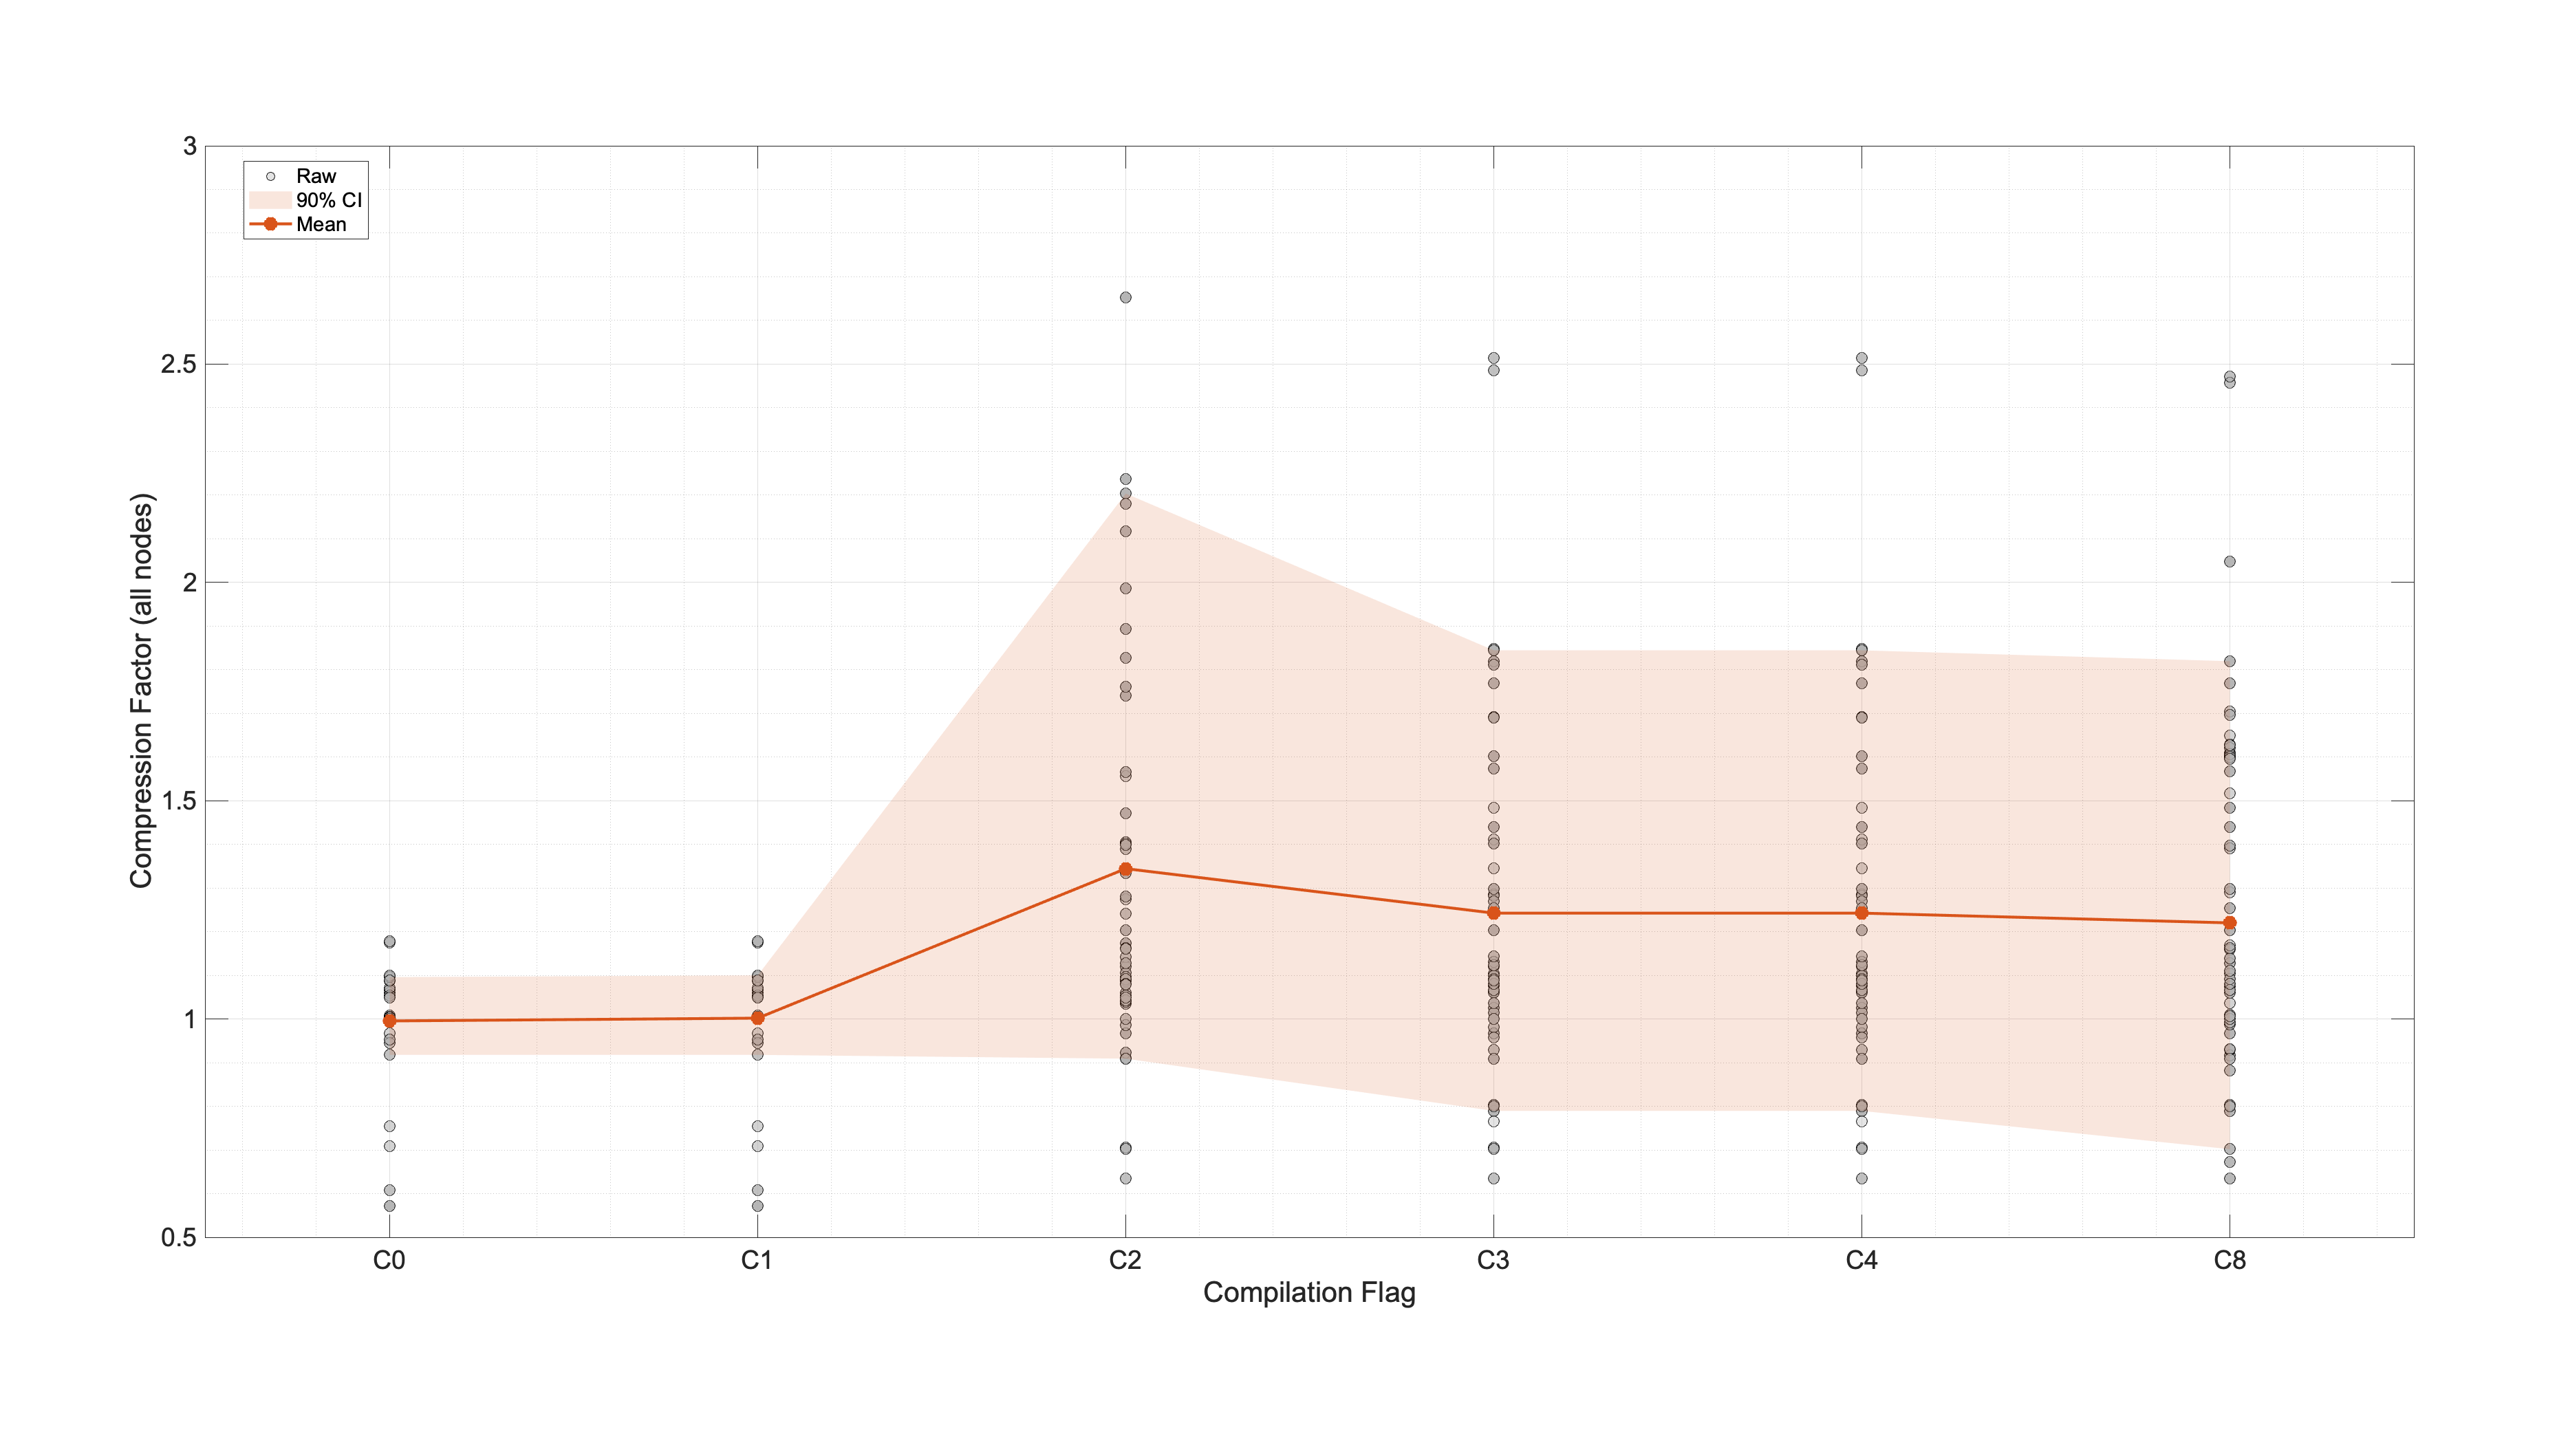
\includegraphics[width=1\textwidth]{figs/compiler/compiler_compression_vs_flag.png}
    \caption{Structural compression factor $\gamma$ (ratio of original to compiled gate count) for each compilation flag $C\ell$.  Grey circles denote individual models; the orange line traces the median and the shaded band covers the 5\,--\,95\,\% quantile range.}
    \label{fig:compiler_compression_levels}
\end{figure}

\begin{table}[t]
  \centering
  \caption{Compression factor $\gamma$ by compilation level $C\ell$.
           Medians are reported together with the $5^{\mathrm{th}}$
           and $95^{\mathrm{th}}$ percentiles.
           Levels $C5$–$C7$ are omitted because no models were compiled
           at those settings in the current benchmark.}
  \label{tab:micro_compilation_flags}
  \begin{tabular}{cccc}
    \toprule
    Compilation flag & Median $\gamma$ & $P_{5}$ & $P_{95}$ \\
    \midrule
    $C0$ & $0.996$ & $0.918$ & $1.096$ \\
    $C1$ & $1.002$ & $0.918$ & $1.100$ \\
    $C2$ & $1.344$ & $0.909$ & $2.204$ \\
    $C3$ & $1.243$ & $0.789$ & $1.844$ \\
    $C4$ & $1.243$ & $0.789$ & $1.844$ \\
    $C8$ & $1.220$ & $0.702$ & $1.820$ \\
    \bottomrule
  \end{tabular}
\end{table}


\paragraph{Key findings.}
\begin{itemize}
  \item Levels $C2$–$C4$ already yield a median $\gamma>1$, confirming
        that early coalescing and Boolean simplification shrink most
        models without full normalization.
  \item Level~$C8$ maintains the compression despite additional passes
        to reach NNF, indicating that late-phase expansions (e.g.,
        DeMorgan pushes) are offset by more aggressive gate
        sharing.
\end{itemize}

% ---------------------------------------------------------------------------
\subsubsection{Compression vs. Average Fan-in}
\label{sec:kc_micro_fanin}
\begin{landscape}
\begin{figure}[hb]
    \centering
    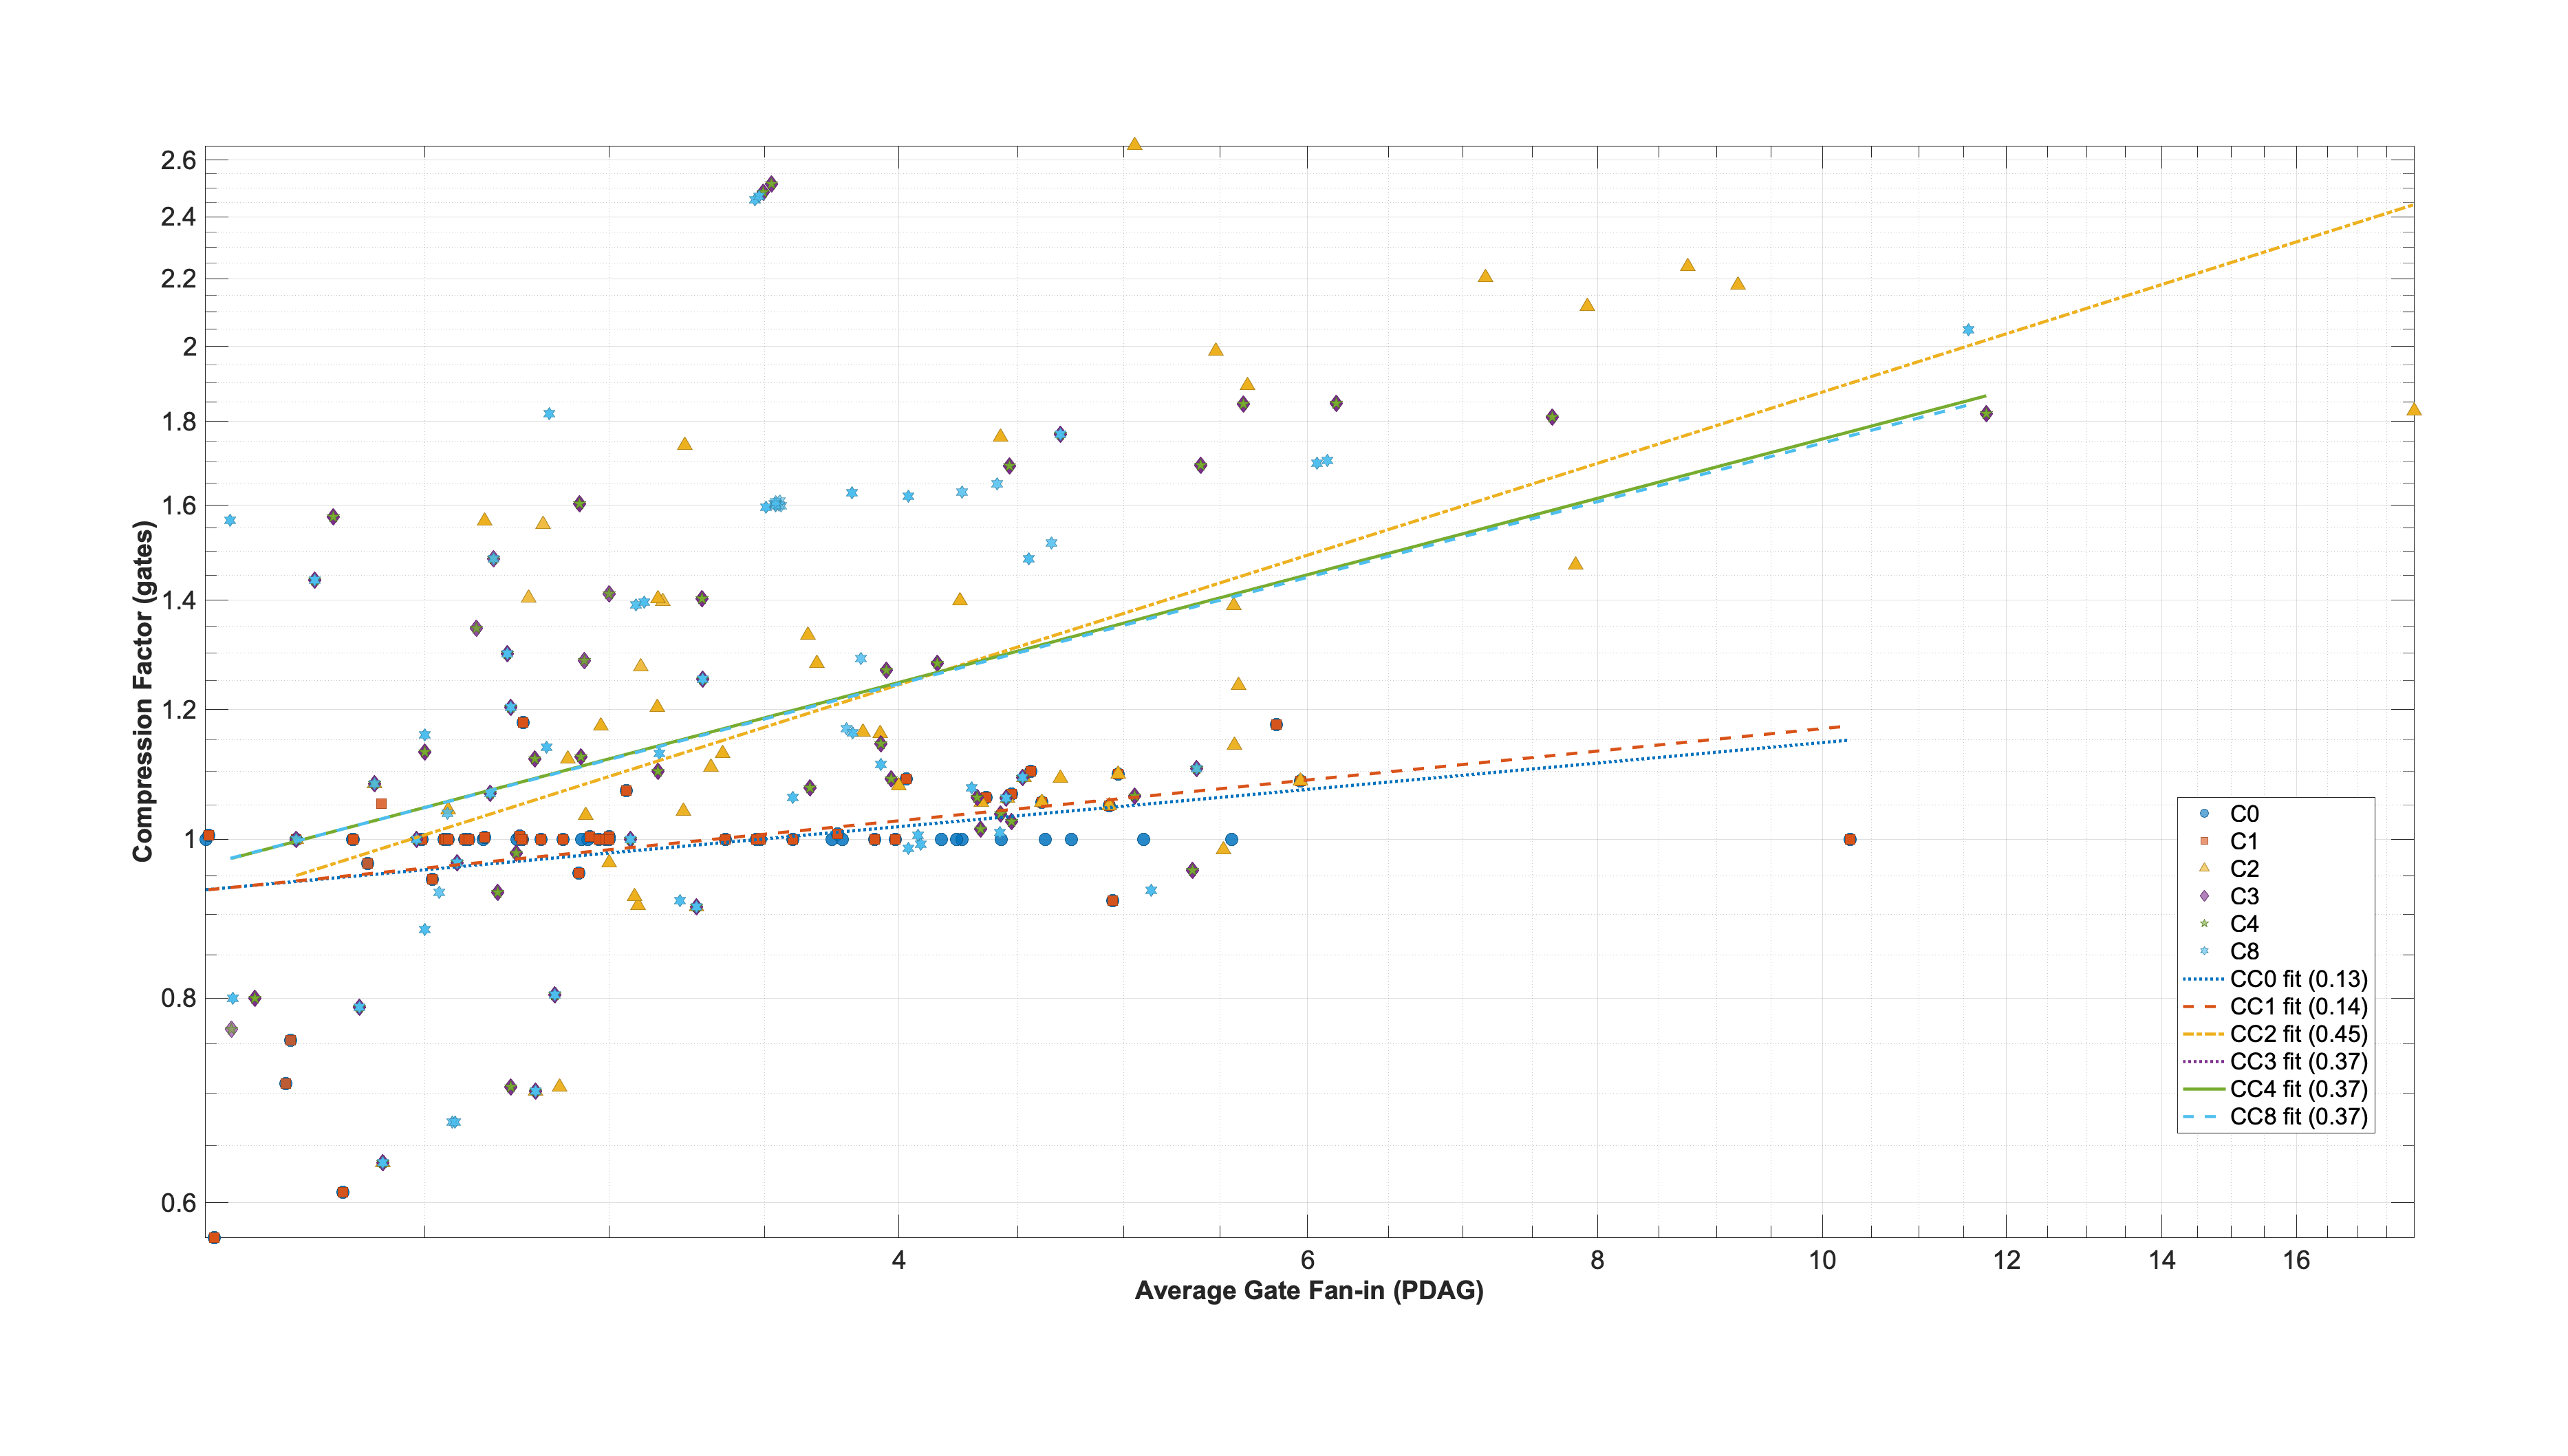
\includegraphics[width=1.15\textwidth]{figs/compiler/compiler_fanin_vs_compression.png}
    \caption{Relationship between average gate fan-in $f$ in the compiled PDAG and structural compression factor $\gamma$.  Points are colored by compilation flag; dashed lines show ordinary least–squares fits on log--log axes with slopes indicated in the legend.}
    \label{fig:compiler_fanin_compression}
\end{figure}
\end{landscape}

Pooling all compilation levels, the relationship between compression
and average gate fan-in $f$ is well described by the log–log regression

\[
  \log_{10}\gamma \;=\; 0.370\,\log_{10}f \; - \; 0.128,
  \qquad R^{2}=0.17\;(n=2064).
\]
Equivalently
$\gamma\approx0.75\,f^{0.37}$, indicating sub-linear returns: doubling
average fan-in improves compression by only $29\%$.

\begin{table}[t]
  \centering
  \caption{Global regression of compression factor on average fan-in.}
  \label{tab:micro_fanin_global}
  \begin{tabular}{lcccc}
    \toprule
    Dataset & Slope $a$ & Intercept $b$ & $R^{2}$ & $n$ \\
    \midrule
    All models & 0.370 & $-0.128$ & 0.17 & 2064 \\
    \bottomrule
  \end{tabular}
\end{table}

The modest $R^{2}$ reflects structural heterogeneity among models: in
series–parallel fragments compression saturates regardless of $f$,
whereas highly redundant safety logic with large voting constructs
exhibits super-linear sharing potential.  A finer taxonomy of these
architectures remains future work.



\chapter{Benchmarks -- Revisited}
% %\input{parts/0_intro/informal_overview}

\chapter{Introduction}
% The entire risk assessment enterprise can be summarized as the act of integrating/bounding uncertainties within what we know to be true. Putting scaffolding around the unknowns. Using the few knowns to better structure the unknowns. To give form to the unknown.
\section{Background \& Motivation}
Probabilistic risk assessment (PRA) aims to quantitatively evaluate the likelihood and severity of adverse events in safety-critical industries. Driven by seminal works such as WASH-1400 and subsequent regulatory guidance, PRA now serves as a cornerstone of risk-informed decision-making in nuclear engineering. A canonical feature of PRA is its reliance on  Boolean logic structures (fault trees and event trees) that characterize sequences of component failures and human actions leading to top-level undesirable outcomes. While such structures ensure thoroughness, the computational complexity of enumerating all failure paths grows exponentially in the number of components. Even moderate-scale reactor models may involve tens of thousands of basic events, rendering naive calculation of end-state probabilities intractable.

Over decades, analysts have adopted a series of approximations and bounding schemes to handle this combinatorial explosion. Strategies include rare-event approximations (which assume minimal overlap between failure sets), min-cut upper bounds (which treat all minimal cut sets as mutually exclusive), and restrictions on gate types to keep expansions manageable. Tools such as CAFTA, FTREX, SAPHIRE, SCRAM, and XFTA implement these methods and remain widely used in industry. Nonetheless, these approximations can lead to conservative estimations.

In recent years, the continued growth of computing power has encouraged reassessment of how PRA calculations can be modernized. Specifically, massively parallel hardware (e.g., GPUs and multi-core CPUs) has prompted the exploration of data-parallel methods. Monte Carlo sampling is a natural fit for parallelization: since each sample is independent, thousands or millions of system-state draws can be processed simultaneously to build empirical estimates of key probabilities. Straightforward sampling from component failures (rather than enumerating complex Boolean expansions) offers flexibility in modeling dependencies and higher-order correlations. The overarching purpose of this dissertation is to develop a data-parallel Monte Carlo framework for large-scale nuclear PRA, grounded in a GPU-friendly integer bit-packing approach and extended to advanced sensitivity analyses using partial derivatives via Shannon decomposition.
\section{Scope}
This work reexamines how to efficiently compute the failure probability of a large Boolean system while capturing a wide array of gate structures, potential dependencies, and partial derivatives for sensitivity. We concentrate on the following core questions:

\begin{itemize}
   \item How can large-scale PRA models be quantified without explicit minimal cut set enumeration or strict reliance on model simplifications?
   \item Which data structures and numerical techniques allow us to exploit parallel hardware such as GPUs, multi-core CPUs, and field-programmable gate arrays (FPGAs)?
   \item What are the current limitations of Monte Carlo (e.g., rare-event estimation and common-cause failure sampling), and how might variance reduction or more sophisticated sampling schemes mitigate them?
\end{itemize}
While our emphasis centers on nuclear applications, the proposed techniques and software are equally suitable for other industries that manage complex risk scenarios (e.g., aerospace, chemical processing, or automotive safety). The dissertation does not attempt to unify every advanced PRA feature (e.g., dynamic simulations or large correlated uncertainties), but it lays the foundation for an extensible data-parallel approach that can incorporate such features in the future.

\clearpage
\section{Outline and Contributions}
The primary technical contributions of this dissertation can be summarized as follows:

\begin{enumerate}
\item \textbf{Data-Parallel Monte Carlo for Boolean Systems:}  
We introduce a new framework that estimates probabilities for all \emph{success} and \emph{failure} states in a single run of Monte Carlo sampling. By representing each random system state in a bit-packed data structure, we achieve high-throughput simulations where Boolean operators (AND, OR, \(k/n\), etc.) map naturally to bitwise operations on GPUs or multi-core CPUs.

\item \textbf{Integration with Probabilistic Circuits:}  
To unify event/fault tree logic with more flexible gate structures, we embed the model in a \emph{probabilistic circuit} representation. This perspective enables node-level factorization and sum mixtures, opening doors to advanced decomposition-based analyses while retaining parallel-friendly evaluation.

\item \textbf{Sampling Techniques for Partial-Derivatives:}  
We develop a bitwise algorithm to approximate partial derivatives of the system’s failure probability with respect to individual or clustered component reliabilities. By evaluating logical expressions under complementary assignments (as guided by the Shannon expansion), these derivatives can be computed in the same Monte Carlo pass. This capability facilitates advanced sensitivity and importance ranking in large models. It also opens a path towards integrating model evaluation with learning-based tasks.

\item \textbf{Benchmarking Against Industry Tools:}  
Through a series of case studies—most notably, the generic pressurized water reactor (PWR) reference model—we compare our approach with standard PRA tools (CAFTA, FTREX, SAPHIRE, SCRAM, XFTA). Results indicate that at comparable accuracy, our framework can surpass existing methods by orders of magnitude in runtime performance. We discuss how discrepancies in extremely low-probability events should be carefully monitored via convergence diagnostics.

\item \textbf{Prototype Implementation:}  
We present an open-source reference implementation named Canopy, built using the SYCL programming model. The code is portable across a variety of parallel architectures, including consumer GPUs and specialized accelerators. We provide usage examples and discuss future directions, such as unifying the approach with importance sampling to better handle rare events and building correlated sampling routines amenable to common-cause failure modeling.
\end{enumerate}

\section{Software Implementations}
\section{Related Publications}
\section{Organization of the Dissertation}
% The remainder of this dissertation is organized into multiple parts covering theoretical foundations, methodological frameworks, practical results, and future directions:

% \begin{itemize}
% \item \textbf{Part I: Foundations}  
%    – Provides an overview of rich Boolean representations (event trees, fault trees) in PRA, introduces probabilistic circuits, and reviews key Monte Carlo sampling principles relevant to reliability estimation.

% \item \textbf{Part II: Proposed Methods}  
%    – Details the data-parallel Monte Carlo approach, discussing bit-packed state encoding, gate-by-gate evaluation, and Shannon-decomposition-based partial derivatives.

% \item \textbf{Part III: Implementation and Results}  
%    – Documents the Canopy software design, GPU kernel formulations, and parallel performance optimizations. Presents numerical benchmarks against large PWR fault-tree models and comparisons with standard PRA codes. Highlights areas needing specialized variance reduction for rare events.

% \item \textbf{Part IV: Extensions and Conclusion}  
%    – Explores potential enhancements, such as correlated sampling for common-cause failures and ways to incorporate Bayesian or machine-learning-based parameter updates. Summarizes major findings and discusses the prospective impact of data-parallel quantification on future PRA methodologies.

% \end{itemize}

% \part{Foundations}

\chapter{Probabilistic Circuits}
\label{chap:boolean_prob_circuits}

\section{Boolean Functions}
\label{sec:boolean_functions}

Let \(\mathbf{x} = (x_1, x_2, \dots, x_n)\) be a vector of \(n\) Boolean variables, where each \(x_i \in \{0,1\}\). A \emph{Boolean function} is a map
\begin{equation}
\label{eq:boolean_function}
F(\mathbf{x}) \;=\; F(x_1, x_2, \dots, x_n) \;\in\; \{0,1\}.
\end{equation}
This function takes each possible configuration of \(\mathbf{x}\) (i.e., each element of \(\{0,1\}^n\)) to a single binary output in~\(\{0,1\}\). Boolean functions appear throughout digital logic, circuit design, and a wide range of computational applications.

For illustration, we can visualize small Boolean functions based on the size of \(\mathbf{x}\). For \(n=1\), there are two possible input states:

\begin{center}
\begin{tikzpicture}
\filldraw[black] (0,0) circle (2pt) node[anchor=north]{\small $x_1=0$};
\filldraw[black] (2,0) circle (2pt) node[anchor=north]{\small $x_1=1$};
\draw[->] (-0.5,0) -- (2.5,0);
\end{tikzpicture}
\end{center}

For \(n=2\), the four possible states can be positioned on a 2D lattice:

\begin{center}
\begin{tikzpicture}[scale=1.5]
\filldraw[black] (0,0) circle (2pt) node[anchor=north east]{\small $(0,0)$};
\filldraw[black] (1,0) circle (2pt) node[anchor=north west]{\small $(1,0)$};
\filldraw[black] (0,1) circle (2pt) node[anchor=south east]{\small $(0,1)$};
\filldraw[black] (1,1) circle (2pt) node[anchor=south west]{\small $(1,1)$};
\draw[->] (-0.5,0) -- (1.5,0);
\draw[->] (0,-0.5) -- (0,1.5);
\end{tikzpicture}
\end{center}

In three dimensions (\(n=3\)), the eight possible states correspond to the vertices of a cube:

\begin{center}
\begin{tikzpicture}[scale=2]
\coordinate (000) at (0,0,0);
\coordinate (001) at (0,0,1);
\coordinate (010) at (0,1,0);
\coordinate (011) at (0,1,1);
\coordinate (100) at (1,0,0);
\coordinate (101) at (1,0,1);
\coordinate (110) at (1,1,0);
\coordinate (111) at (1,1,1);

\foreach \point in {(000),(001),(010),(011),(100),(101),(110),(111)}
    \filldraw[black] \point circle (0.5pt);

\draw (000) -- (100) -- (110) -- (010) -- (000);
\draw (001) -- (101) -- (111) -- (011) -- (001);
\draw (000) -- (001);
\draw (100) -- (101);
\draw (110) -- (111);
\draw (010) -- (011);

\node[anchor=north east] at (000) {\small $(0,0,0)$};
\node[anchor=north west] at (100) {\small $(1,0,0)$};
\node[anchor=south east] at (010) {\small $(0,1,0)$};
\node[anchor=south west] at (110) {\small $(1,1,0)$};
\node[anchor=north east] at (001) {\small $(0,0,1)$};
\node[anchor=north west] at (101) {\small $(1,0,1)$};
\node[anchor=south east] at (011) {\small $(0,1,1)$};
\node[anchor=south west] at (111) {\small $(1,1,1)$};
\end{tikzpicture}
\end{center}

Boolean operators such as AND (\(\land\)), OR (\(\lor\)), and NOT (\(\lnot\)) allow constructing a wide variety of logical relationships. For example, in a setting where a system fails if any one of two components fails, the Boolean function can be written as
\[
F(x_A, x_B) \;=\; x_A \;\lor\; x_B.
\]
Here, \(F=1\) precisely when \(x_A=1\) or \(x_B=1\), encompassing a failure event if either component \(A\) or \(B\) is in state 1. More complex systems with many interdependent components may require Boolean functions with numerous variables and deeply nested operators.

Although Boolean functions are crucial for representing logical configurations, they operate purely in a binary framework and do not directly encode probability distributions. To include probabilistic behavior, we can move to a more expressive framework called \emph{probabilistic circuits}, which describe the distribution of variables in a directed acyclic graph (DAG). Such representations can capture both the combinatorial structure of system states and the uncertainty or likelihood associated with these states.

\section{Definition and Structure}

Consider a set of random variables \(\mathbf{X} = (X_1, X_2, \dots, X_n)\). A \emph{probabilistic circuit} \(\mathcal{C}\) is a DAG whose nodes consist of:

\begin{itemize}
 \item \textbf{Input nodes (leaves):} Each leaf encodes a base distribution over some subset of \(\mathbf{X}\). Often, these leaves correspond to univariate distributions \(p(X_i)\) or constant/indicator functions.
 \item \textbf{Internal nodes (gates):} Each gate combines incoming distributions from its children using either:
   \begin{itemize}
   \item \textbf{Sum-gates (mixture gates):} Weighted sums of child distributions, with nonnegative weights summing to 1.
   \item \textbf{Product-gates:} Factorized products of child distributions, each child covering disjoint subsets of \(\mathbf{X}\).
   \end{itemize}
\end{itemize}
The acyclic nature of the graph ensures that information flows consistently from the leaves toward a designated \emph{root} node.

\subsection{Sum-Gates and Product-Gates}

Let \(v\) be an internal node in \(\mathcal{C}\). Denote the children of \(v\) by \(\operatorname{ch}(v)\). Then:

\begin{itemize}
\item \textbf{Sum-gate:} Suppose \(v\) has children \(u_1,\dots,u_k\) with mixture weights \(\{\theta_{v,u_i}\}_{i=1}^k\) satisfying \(\sum_{i=1}^k \theta_{v,u_i} = 1\) and \(\theta_{v,u_i} \ge 0\). The distribution encoded at \(v\) is
\begin{equation}
\label{eq:sum_gate}
p_v(\mathbf{x}) \;=\; \sum_{i=1}^k \theta_{v,u_i}\,p_{u_i}(\mathbf{x}),
\end{equation}
where \(p_{u_i}(\mathbf{x})\) is the distribution encoded by child node \(u_i\).

\item \textbf{Product-gate:} Suppose \(v\) has children \(u_1,\dots,u_k\), each covering disjoint subsets of \(\mathbf{X}\). Let \(\mathbf{X}=\bigcup_{i=1}^k \mathbf{X}_{u_i}\) and \(\mathbf{X}_{u_i}\cap \mathbf{X}_{u_j} = \varnothing\) for \(i\neq j\). Then the distribution at \(v\) is
\begin{equation}
\label{eq:product_gate}
p_v(\mathbf{x})
\;=\;
\prod_{i=1}^k
p_{u_i}\bigl(\mathbf{x}_{u_i}\bigr),
\end{equation}
where \(\mathbf{x}_{u_i}\) is the restriction of \(\mathbf{x}\) to the variables in \(\mathbf{X}_{u_i}\).
\end{itemize}

\subsection{Leaf Nodes and the Circuit Distribution}

Each leaf node encodes a base distribution over its subset of variables (or a constant/indicator). Let \(v\) be a leaf node associated with \(p_v(\mathbf{X}_v)\). When the circuit is evaluated, each leaf contributes its assigned distribution or constant term. By recursively composing sum-gates and product-gates, every node \(v\) in the circuit defines a distribution \(p_v(\mathbf{x})\). The distribution of the entire circuit is given by evaluating its \emph{root} node \(r\):
\[
p_r(\mathbf{x}) \;=\; \text{(\(r\) evaluated from the leaves up)}.
\]

Probabilistic circuits unify structural and probabilistic modeling in a single formalism. They are widely used in fields such as artificial intelligence, machine learning, and automated reasoning, offering a tractable way to represent complex, high-dimensional probability distributions while preserving interpretable, compositional structure.


\input{parts/1_foundations/1_PRA/0_intro}
\input{parts/1_foundations/1_PRA/1_ET}
\input{parts/1_foundations/1_PRA/2_FT}


\usetikzlibrary {intersections}
\usetikzlibrary {graphs}
\begin{figure}[ht!]
\centering
\begin{tikzpicture}[domain=-4:12]
  % \draw [help lines] (-4,0) grid (12,12);
  \draw[->] (-4.0,0) -- (11,0) node[right] {$x$};
  \draw[->] (-4,0) -- (-4,12.0) node[above] {$f(x)$};
\begin{scope}[every node/.style={thick}]
    \node (ss_begin) at (-2.75,1.75) {$\text{S}_0$};

    \node (ss_end) at (9.5,11.0) {$\text{ES}_{0}$} ;
    % \node (ss_1) at (2.5,0.0) {$S_1$};
    % \node (ss_i) at (5.0,0.0) {$S_i$};
    % \node (ss_j) at (10.0,0.0) {$S_j$};
    % \node (ss_jp1) at (12.5,0.0) {$S_{j+1}$};

\end{scope}

\begin{scope}[>={Circle[black]},
              every edge/.style={draw=black,very thick}]
    % \path [->] (ss_0) edge (ss_1);
    % \path [->] (ss_1) edge (ss_i);
    % \path [->] (ss_i) edge (ss_j);
    % \path [->] (ss_j) edge (ss_jp1);
    % \path [->] (ss_jp1) edge (ss_f);
    % %\path [->] (B) edge node {$3$} (C);
    %\path [<->] (ss_begin) edge[out=25,in=220] node {} (ss_ie_i); 
    \path[<->,save path=\pathA,name path=A] (ss_begin) to [out=45,in=160, edge node={node [near end, above] {$\text{S}_0$}}](ss_end);

    \path[<->,save path=\pathB,name path=B] (1,0) to (1,11);

  \fill[name intersections={of=A and B}] (intersection-1) circle (3pt);

  \node[anchor=south east] (ss_ie_i) at (intersection-1) {$\text{IE}_i$};

  \draw[<->,black,very thick][use path=\pathA];
  %\draw[red] [use path=\pathB];
    %\path [<->] (ss_begin) edge[out=25,in=180] node[near end, above] {$\text{S}_0$} (ss_end); 
    %\path [<->] (ss_ie_i) edge[out=0,in=180] node[sloped] {} (ss_end); 
\end{scope}
\begin{scope}
  [grow'=right,
   level distance=50pt,
   every tree node/.append style={anchor=base west},
   execute at begin node=\strut,
   level 0/.style={sibling distance=0pt},  % initiating event
   level 1/.style={sibling distance=55pt}, %
   level 2/.style={sibling distance=45pt},
   level 3/.style={sibling distance=25pt, nodes={right=2}},
   edge from parent/.append style={
        draw,
        edge from parent path={
            (\tikzparentnode.east) -| ($(\tikzparentnode.east)!0.5!(\tikzchildnode.west)$) |- (\tikzchildnode.west)
        },
    },
    every node/.append style={anchor=center,font=\small,text centered},
    % every level 0 node/.append style={circle, font=\small\bfseries, draw, fill=blue!30, inner sep=0pt},
    every leaf node/.append style={nodes={right=2}},
   ]
   \graph
{
  "$I$"[at={(intersection-1)}, right=1.25] -> {
    b -> c
  };
};

  % \node at (intersection-1)[right=1.25]{$I$}
  %    child {node {$F_{1}^s$}
  %      child {node {$F_{2}^s$}
  %        child {node {$\text{ES}_{1}$}}
  %      }
  %      child {node {$F_{2}^f$}
  %        child {node {$\text{ES}_{2}$}}
  %        child {node {$\text{ES}_{3}$}}
  %      }
  %    }
  %    child {node  {$F_{1}^f$}
  %      child {node {$\text{ES}_{4}$}}

  \end{scope}   
\end{tikzpicture}
\end{figure}

\chapter{Probability Estimation using Monte Carlo Sampling}
\section{Monte Carlo Fundamentals}
Monte Carlo methods provide a versatile framework for approximating expectations, probabilities, and other quantities of interest by simulating random observations from an underlying distribution. At its core, a Monte Carlo estimator uses repeated random draws to approximate quantities such as
\begin{equation}
\label{eq:generic_monte_carlo_estimator}
\mathbb{E}[f(X)]
\;=\;
\int f(x)\,p(x)\,\mathrm{d}x
\;\;\approx\;\;
\frac{1}{N}\sum_{i=1}^N f\bigl(x^{(i)}\bigr),
\end{equation}
where \(x^{(1)},x^{(2)},\dots,x^{(N)}\) are independent and identically distributed (i.i.d.) samples drawn from \(p\). The function \(f\) is a measurable function of the random variable \(X\). In reliability and PRA contexts, \(f\) might be an indicator of a particular event (e.g., a system failure), in which case \(\mathbb{E}[f(X)]\) becomes the probability of that event.
\subsection{Convergence and the Law of Large Numbers}
A central theoretical result underpinning Monte Carlo sampling is the \emph{Law of Large Numbers (LLN)}. In one of its classical forms, the Strong LLN states:
\begin{theorem}[Strong Law of Large Numbers]
\label{thm:SLLN}
Let \(X_1, X_2, \dots\) be a sequence of i.i.d.\ random variables with finite expectation \(\mathbb{E}[X_1]\). Then, with probability 1,
\[
\lim_{N\to\infty}
\frac{1}{N}\sum_{i=1}^N X_i
\;=\;
\mathbb{E}[X_1].
\]
\end{theorem}
Applied to the sample estimator in Eq.~\eqref{eq:generic_monte_carlo_estimator}, the LLN implies that as the number of samples \(N\) grows large, the average of the function values \(f\bigl(x^{(i)}\bigr)\) converges to \(\mathbb{E}[f(X)]\). Thus, by simply drawing enough samples, one can approximate probabilities or expectations arbitrarily well (with probability~1).

\subsection{Central Limit Theorem and Error Analysis}
Another classical result is the \emph{Central Limit Theorem (CLT)}, which indicates that the Monte Carlo estimator’s distribution (around its true mean) approaches a normal distribution for large \(N\). Specifically,

\begin{theorem}[Central Limit Theorem]
\label{thm:CLT}
Suppose \(X_1, X_2,\dots\) are i.i.d.\ random variables with mean \(\mu=\mathbb{E}[X_1]\) and variance \(\sigma^2=\mathbb{V}[X_1]<\infty\). Then the sample mean satisfies
\[
\sqrt{N}
\biggl(
 \frac{1}{N}\sum_{i=1}^N X_i - \mu
\biggr)
\;\;\xrightarrow{\mathrm{d}}\;\;
\mathcal{N}(0,\sigma^2),
\]
where \(\xrightarrow{\mathrm{d}}\) denotes convergence in distribution.
\end{theorem}

In practical terms, the CLT implies that for sufficiently large \(N\), the sampling fluctuations of the Monte Carlo estimator around the true mean are approximately normal. The variance of this normal distribution decreases with \(1/N\). Therefore, one can estimate confidence intervals, standard errors, and convergence rates by tracking empirical variance across the sample.

The above principles remain valid even when \(f\) is an indicator of a Boolean event or a composite system failure embedded in an event/fault tree. One need only be able to draw samples \(\bigl(x^{(i)}\bigr)\) from the system’s joint distribution over basic events (or from any suitable representation of the PRA model) and then evaluate the function \(f\) to determine system success/failure for each sample. Subsequent chapters will expand on how these samples can be generated for event trees, fault trees, or more complex DAG-based representations.

\section{Random Number Generation and Random Variates}
Monte Carlo estimators rely on the ability to generate random realizations from a given distribution. Computers, however, do not typically provide true randomness; instead, they use \emph{pseudo}-random number generators (PRNGs) to produce sequences of numbers that mimic realizations from a uniform distribution on \([0,1]\). From these \emph{uniform} samples, one can then derive samples from more general distributions using various transformations (e.g., the \emph{inverse transform} method, acceptance-rejection, composition methods, or specialized sampling algorithms).

\subsection{Pseudo-Random Number Generation}
A PRNG is formally a deterministic function that, given an initial \emph{seed}, generates a long sequence of values in \((0,1)\). Popular choices include:
\begin{itemize}
\item \emph{Linear Congruential Generators (LCG)}, which use a recurrence of the form
\[
X_{n+1}
\;=\;
(a\,X_n + c)
\;\bmod\; m,
\]
then normalize \(\frac{X_{n+1}}{m}\) to produce a pseudo-random variate in \((0,1)\).
\item \emph{Mersenne Twister}, which generates high-quality pseudo-random numbers with a very long period (e.g., \(2^{19937}-1\)).
\item \emph{Philox} or other counter-based methods that deliver high performance and reproducible streams across parallel computations.
\end{itemize}

While these methods provide deterministic sequences, strong design ensures that the resulting outputs pass numerous statistical tests for randomness. If the seed is chosen randomly (or from a secure source), these methods can approximate uniformity closely enough for most Monte Carlo studies.

\subsection*{Random Variates via Transformations}
Given access to uniform samples \(U\sim \mathrm{Unif}(0,1)\), one can construct samples from many other distributions. Two widely used techniques are:

\begin{enumerate}
\item \textbf{Inverse Transform Sampling:}  
   Suppose a continuous variable \(X\) has cumulative distribution function (CDF) \(F_X(x)\). If \(U\sim \mathrm{Unif}(0,1)\), then \(X=F_X^{-1}(U)\) follows the same distribution as \(X\). More precisely,
   \[
   P\bigl[X \le x\bigr]
   \;=\;
   P\bigl[F_X^{-1}(U)\le x\bigr]
   \;=\;
   P\bigl[U \le F_X(x)\bigr]
   \;=\;
   F_X(x),
   \]
   provided \(F_X\) is continuous and strictly increasing.  

\item \textbf{Acceptance-Rejection:}  
   For certain distributions where the inverse CDF is not straightforward, one can sample from an easier \emph{proposal distribution} \(q(x)\) that bounds the targeted density \(p(x)\). Specifically, if \(p(x)\le M\,q(x)\) for all \(x\), then:
   \begin{enumerate}
   \item Draw \(Y\sim q(\cdot)\) and \(Z\sim \mathrm{Unif}(0,1)\).
   \item Accept \(Y\) if \(Z\le \frac{p(Y)}{M\,q(Y)}\). Otherwise, reject and repeat.
   \end{enumerate}
   The accepted sample \(Y\) follows distribution \(p(x)\).  
\end{enumerate}

\subsection{Boolean Events as Discrete Random Variables}
In PRA contexts, many variables are \emph{discrete}, often Bernoulli (success/failure) or categorical (e.g.\ multiple failure modes). Generating \(\{0,1\}\)-valued samples is then straightforward, since for each basic event \(b\),
\[
\Pr[b=1] \;=\; p(b),
\quad
\Pr[b=0] \;=\; 1-p(b).
\]
Given a uniform variate \(U\), one sets
\[
b
\;=\;
\begin{cases}
1, & U \le p(b),\\
0, & \text{otherwise}.
\end{cases}
\]
This approach naturally extends to multi-categorical events. More complex dependencies among events can also be captured by specifying appropriate conditional distributions.

\subsection{Extending Boolean Events to Continuous Random Variables}
A \emph{continuous} random variable \(Y\) has a probability density function (PDF) \(f_Y(y)\) on a continuous domain \(\mathcal{Y}\subseteq \mathbb{R}\). Common examples in reliability include:
\begin{itemize}
\item \textbf{Exponential Distribution}, often used to model times to failure under a constant hazard rate \(\lambda\). Its PDF is
\[
f_Y(y) \;=\; \lambda\, e^{-\lambda y},
\quad
y \ge 0.
\]
\item \textbf{Weibull Distribution}, with flexible shape parameter \(\beta>0\) and scale parameter \(\alpha>0\). Its PDF is
\[
f_Y(y)
\;=\;
\frac{\beta}{\alpha}
\Bigl(\frac{y}{\alpha}\Bigr)^{\!\beta -1}
\exp\!\biggl[-\bigl(y/\alpha\bigr)^{\!\beta}\biggr],
\quad
y\ge 0.
\]
\item \textbf{Lognormal Distribution}, where \(\log(Y)\) follows a normal distribution. This is sometimes employed for components whose lifetimes span multiple orders of magnitude.
\end{itemize}
In a PRA context, continuous random variables typically arise when modeling the \emph{time dimension}: for instance, the time until a valve sticks closed, or the moment when a pipe experiences a critical crack. One can then generate a Bernoulli indicator for whether the failure has occurred by time \(t\) using
\[
\Pr[Y \le t]
\;=\;
\int_{0}^{t} f_Y(y)\,\mathrm{d}y
\;=\;
F_Y(t),
\]
where \(F_Y\) is the cumulative distribution function (CDF) of \(Y\). Evaluating this probability at each Monte Carlo trial and comparing against a uniform random variate yields a discrete failure indicator. Hence, continuous distributions can be mapped to discrete states at any chosen time horizon.




\subsubsection*{Ensuring Reliable Sampling in High-Dimensional Boolean Spaces}
When dealing with large-scale PRA models or deeply nested Boolean structures (multiple fault trees and event trees), a careful approach to random variate generation is needed:
\begin{itemize}
\item \textbf{Reusable Streams:} Use a consistent seeding and PRNG strategy to ensure reproducibility of results, especially when comparing multiple system configurations.
\item \textbf{Parallel and Distributed Simulations:} Avoid overlapping random streams (i.e., ensure different parallel processes use uncorrelated seeds).
\item \textbf{Validation of Randomness:} Use standard test suites (e.g.\ TestU01, Diehard) if the model’s accuracy depends on fine-scale statistical properties.
\end{itemize}
Once random variates for each basic event are generated, higher-level logical structures (e.g.\ gates in a fault tree or branches in an event tree) can be evaluated deterministically.  Subsequent sections will address how to form either a single \emph{global} sample of all events in the system or to \emph{factorize} the sampling process according to the structure of the DAG-based PRA model.

\chapter{Problem Statement}


% \begin{figure}
% \begin{tikzpicture}
%   \graph [nodes={align=center, inner sep=1pt}, grow right=1.5]
% {
%   a,
%   b,
%   c -> d -> {
%     e -> f -> g,
%     h -> i
%   } -> j,
%   k -> l
% }
% \end{tikzpicture}
% \caption{An illustrative “success tree,” showing how multiple mitigation paths from the initial condition \(S_0\) can lead to safe or acceptable outcomes.}
% \label{fig:success_tree_example}
% \end{figure}
% Match the style from fig:event_tree_example
% \tikzset{grow'=right,level distance=48pt}
% %\tikzset{execute at begin node=\strut}
% %\tikzset{every tree node/.style={anchor=base west}}
% \tikzset{
%     edge from parent/.append style={very thick},
%     edge from parent/.style={
%         draw,
%         edge from parent path={
%             (\tikzparentnode.east) -| ($(\tikzparentnode.east)!0.5!(\tikzchildnode.west)$) |- (\tikzchildnode.west)
%         },
%     },
%     every node/.style={circle, minimum width=0.2cm, draw, anchor=center,font=\small\bfseries, text centered},
%     %every level 0 node/.style={circle, font=\small\bfseries, draw, fill=blue!30, inner sep=0pt},
%     %every internal node/.style={font=\small, inner sep=4pt},
%     %every leaf node/.style={rectangle, draw, fill=blue!30, minimum width=2.5cm, text centered},
%     %frontier/.style={distance from root=400pt},
% }
% \Tree [.\(1\)
%     [.\(F_1^{\text{fail}}\)
%         [.\(X_3\) ]
%     ]
% ]
% \Tree [.\(I\)
%     [.\(F_1^{\text{succ}}\)
%         [.\(F_2^{\text{succ}}\)
%             [.\(X_1\) ]
%         ]
%         [.\(F_2^{\text{fail}}\)
%             [.\(X_2\) ]
%         ]
%     ]
%     [.\(F_1^{\text{fail}}\)
%         [.\(X_3\) ]
%     ]
% ]
% Example success tree
% \Tree [.\(S_0\)
%     [.\(Mitigation \#1\)
%         [.\(Mitigation \#2\)
%             [.\(\text{Full Success}\) ]
%         ]
%         [.\(Alternate\)
%             [.\(\text{Partial Success}\) ]
%         ]
%     ]
%     [.\(Backup\)
%         [.\(\text{Alternate Success}\) ]
%     ]
% ]

% \part{A Brute Force Approach}
\large{\begin{hindi}
नर हो, न निराश करो मन को \\
कुछ काम करो, कुछ काम करो
\end{hindi}}
\chapter{Model Representation}

\input{parts/2_bruteforce/1_representation/1_DAG}
\input{parts/2_bruteforce/1_representation/2_alt_forms}
\chapter{Building a Data-Parallel Monte-Carlo Probability Estimator}

\input{parts/2_bruteforce/2_estimator/1_overview}

\input{parts/2_bruteforce/2_estimator/2_prng}

\section{Preliminary Benchmarks}

\input{parts/2_bruteforce/3_benchmark/3_table_aralia_ft_dataset}

\input{parts/2_bruteforce/3_benchmark/3_setup}

\clearpage
\begin{landscape}
\begin{figure}[h]
    \centering
    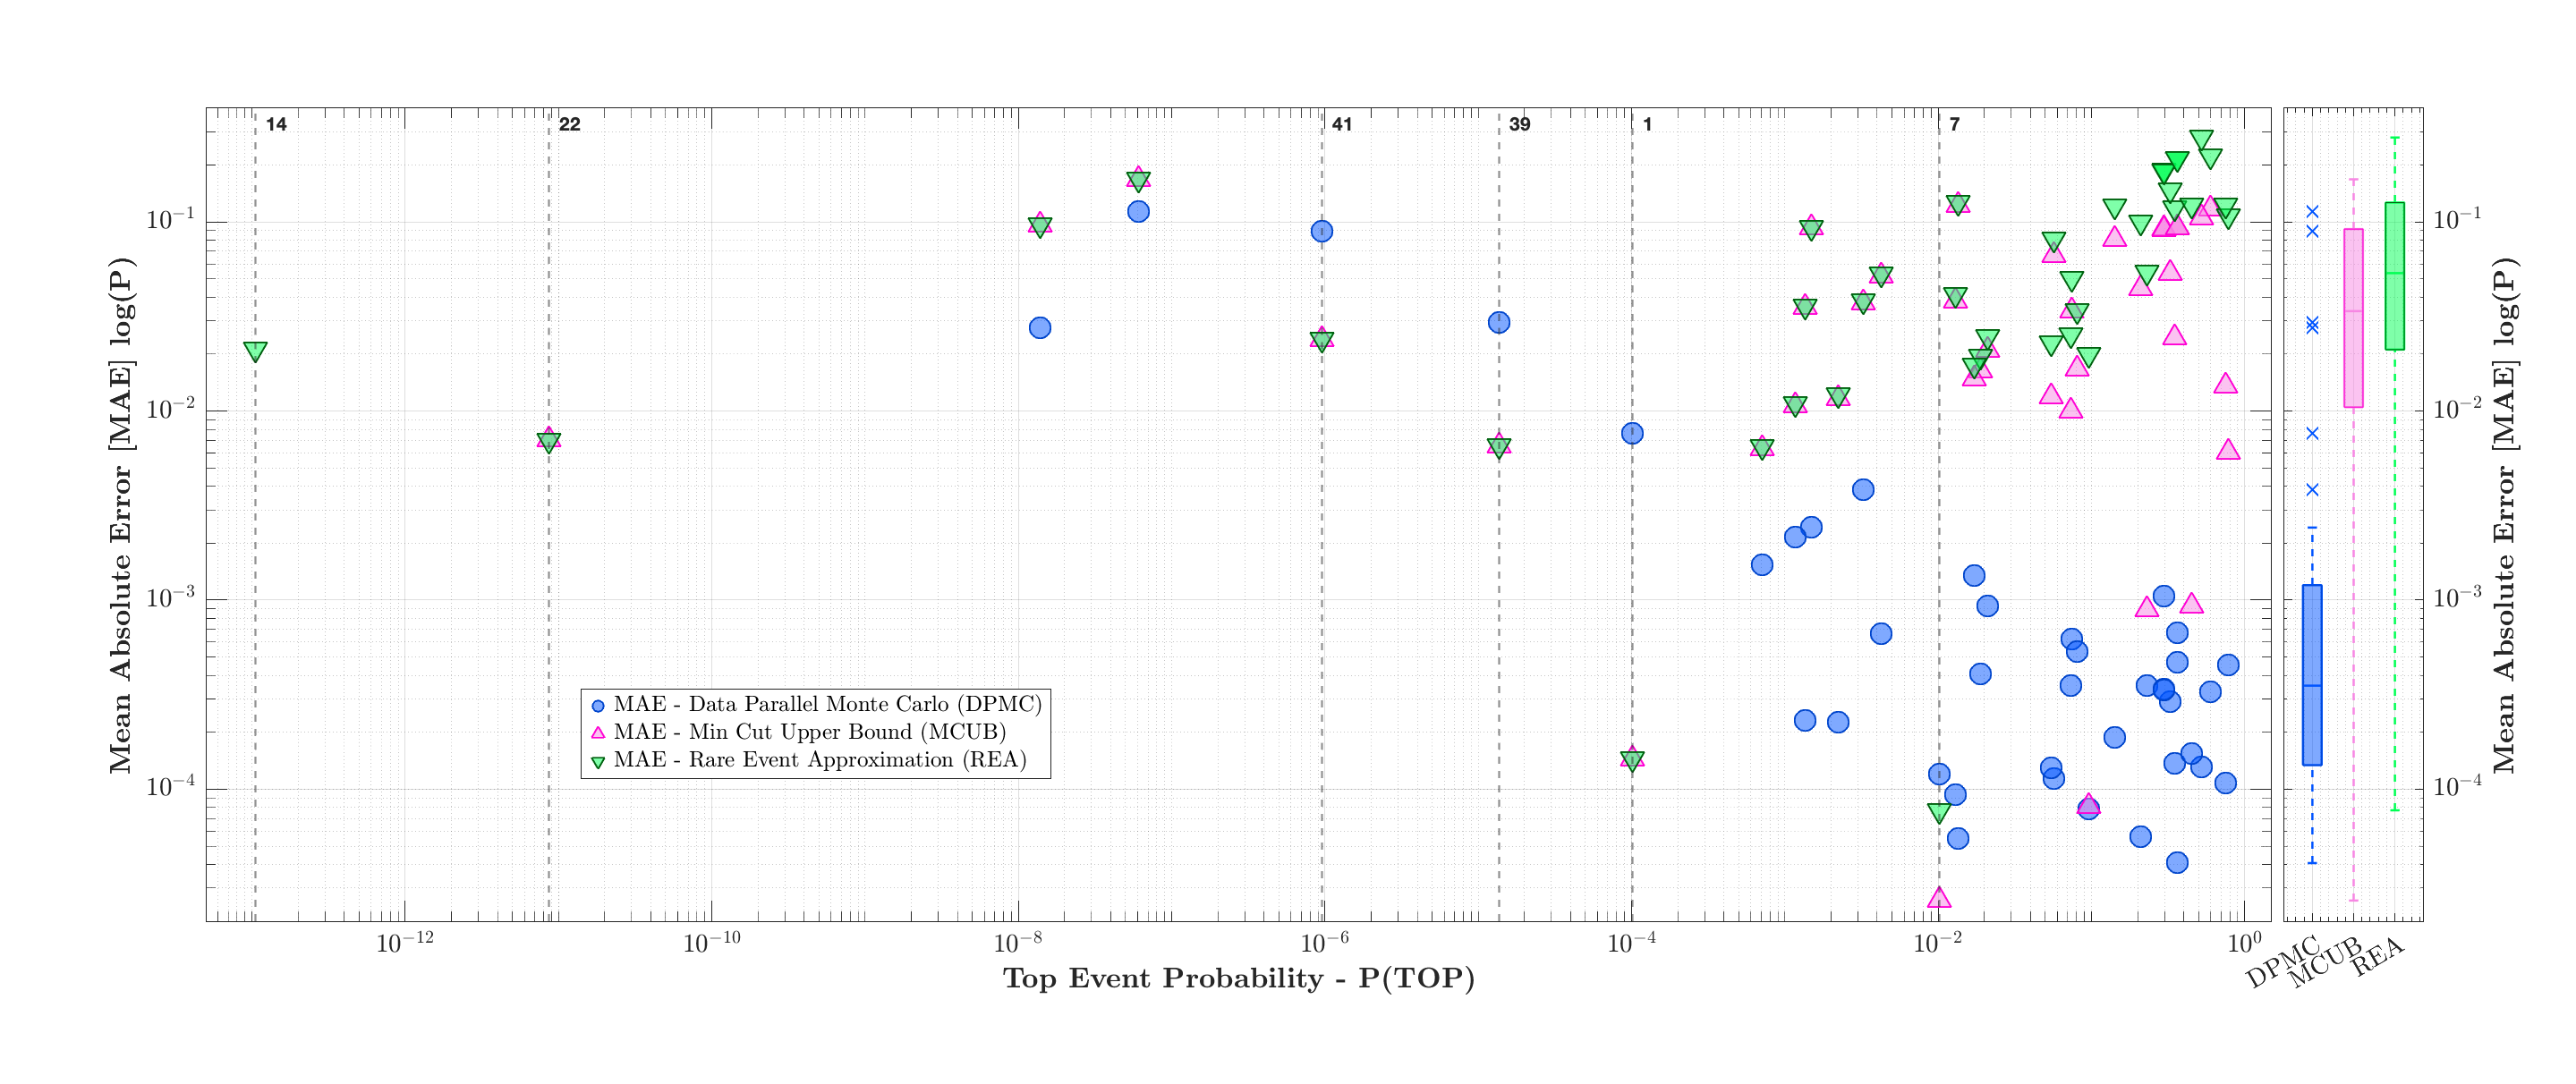
\includegraphics[width=1.2\textwidth]{parts/2_bruteforce/3_benchmark/error_vs_prob_detailed.png}
    \caption{Mean Absolute Error – Exact (BDD) vs Approximate Methods}
    \label{fig:mae_vs_logp}
\end{figure}
\end{landscape}

\input{parts/2_bruteforce/3_benchmark/4_mae}

% \part{Refinements}
\begin{sanskrit}
करत करत अभ्यास, जड़मति होत सुजान
\end{sanskrit}

\chapter{Variance Reduction}
\section{Dealing with Rare Events using Importance Sampling}
\subsection{Interplay between ultra-rare and ultra-frequent events - how they affect convergence}
\section{Sampling Correlated Events}
\chapter{Hardware Optimizations}

\input{parts/3_refinements/2_hw_opt/1_voter/_}

\part{Learning}

\chapter{Towards Parameter Learning}
\label{sec:parametric_learning_pra_model}

PRAs invariably involve uncertainty. When explicitly modeled, these uncertainties can be updated or inferred from evidence, engineering judgments, or reliability targets. We refer to such systematic updating of probability or frequency distributions across the PRA model as form of parametric learning.

Recall from (Section~\ref{sec:unified_pra_dag}) that we represent a PRA model as a PDAG. Let \(\boldsymbol{\theta}\) be the collection of parameters governing all relevant probabilities/frequencies in this PDAG. For an end-state \(S_j\), the model-based prediction under \(\boldsymbol{\theta}\) is
\[
P_{\mathcal{M}}\bigl(S_j \mid \boldsymbol{\theta}\bigr).
\]
If one also has observed or target frequencies \(\bigl\{p_{j}^{\mathrm{obs}}\bigr\}\), parametric learning seeks to reconcile this information with the model’s predictions by updating \(\boldsymbol{\theta}\). In a Bayesian setting, one may specify a prior distribution over \(\boldsymbol{\theta}\) and update this prior to a posterior distribution via the likelihood of observed end-state frequencies or other system-level evidence. Alternatively, one may adopt an optimization-based approach: define a loss or cost function that measures the discrepancy between \(\{p_{j}^{\mathrm{obs}}\}\) and \(\{P_{\mathcal{M}}(S_j \mid \boldsymbol{\theta})\}\), then minimize this loss with respect to \(\boldsymbol{\theta}\). Both perspectives aim to systematically adjust the PRA model’s probabilistic parameters so that end-state frequencies (or other risk metrics) remain consistent with available data or requirements. 

In the next section, we show how parametric learning over the PDAG can be setup as a constrained optimization problem.

\section{Parameter Learning as Constrained Optimization}
\label{sec:opt_formalization}

Each node \(X_i\) in the PDAG has an associated parameter \(\theta_i\), gathered into a vector  
\[
\boldsymbol{\theta}
\;=\;
(\theta_1,\;\theta_2,\;\dots,\;\theta_n).
\]
For a set of end-states \(\{S_j\}_{j=1}^m\), the model’s predicted probability under \(\boldsymbol{\theta}\) is  
\[
p_{j}^{\mathrm{pred}}\bigl(\boldsymbol{\theta}\bigr)
\;=\;
P_{\mathcal{M}}\bigl(S_j \mid \boldsymbol{\theta}\bigr).
\]
Suppose observed or target frequencies \(\bigl\{p_{j}^{\mathrm{obs}}\bigr\}\) are given. A discrepancy measure  
\[
d\!\bigl(p_{j}^{\mathrm{obs}},\,p_{j}^{\mathrm{pred}}(\boldsymbol{\theta})\bigr)
\]
compares the model’s predictions to these values. One can also add a regularization term \(\Psi(\boldsymbol{\theta})\) to encode additional constraints such as engineering limits or prior information. Let \(\Omega\) denote the feasible set for \(\boldsymbol{\theta}\), enforcing domain-specific requirements (e.g., probability normalization). Parameter learning then becomes the following constrained optimization problem:
\[
\min_{\boldsymbol{\theta} \,\in\, \Omega} 
\quad 
\sum_{j=1}^m
d\!\Bigl(
   p_{j}^{\mathrm{obs}},\,
   p_{j}^{\mathrm{pred}}(\boldsymbol{\theta})
\Bigr)
\;+\;
\Psi(\boldsymbol{\theta}).
\]
A solution \(\boldsymbol{\theta}^{*}\) in \(\Omega\) is sought that minimizes overall discrepancy while respecting any additional constraints. Gradient-based methods (when \(d\) is differentiable) or other solvers can be employed.

\input{parts/4_learning/1_param/1_demo}
\input{parts/4_learning/1_param/3_case_study}
\input{parts/4_learning/1_param/4_figs}

\section{Transformations}
\input{2_foundations/knowledge_compilation/transformation/as_nnf}
\input{2_foundations/knowledge_compilation/transformation/as_dnf_tree}
\input{2_foundations/knowledge_compilation/transformation/as_cnf}
\input{2_foundations/knowledge_compilation/transformation/as_dnnf}
% \subsection{\color{blue}{And-Inverter Graphs}}
\input{2_foundations/knowledge_compilation/transformation/as_dd/_}

\printbibliography[
heading=bibintoc,
title={References}
]
\appendix

%%---------------------------------------------------------------------------%%
%%  Bibliography 
%% or use BibTeX
% \bibliography{references}
% \bibliographystyle{apalike}

%%---------------------------------------------------------------------------%%
% Appendices
%\ensureoddstart
\restoregeometry
\backmatter
% \appendix
% 

\chapter{Revised Aralia Benchmark Plots}

In this chapter, we plot the the Monte--Carlo convergence experiments on the \emph{Aralia} fault--tree data set (Section~\ref{subsec:aralia_dataset}).  The revised study targeted a relative margin of error of $0.1\%$, that is, $\varepsilon = 10^{-3}\,\hat{p}$, at a $99\,\%$ confidence level with a wall--clock time limit of 60~s per model. The following figures collate the updated convergence traces for all 43 fault trees.

\begin{itemize}
  \item the sample mean estimate (solid colored line),
  \item the empirical $90\,\%$ and $99\,\%$ confidence bands (shaded regions)
  \item where available, the reference ``oracle/true'' probability (black dashed).
\end{itemize}


\begin{landscape}
\foreach \i in {1,...,9}{%%
  \begin{figure}[p]
      \centering
      \includegraphics[width=1\textwidth]{figs/convergence/e001p99/conv_fig_0\i.png}
      \caption{Aralia Fault Tree \i}
      \label{fig:conv_fig_\i}
  \end{figure}
}

\foreach \i in {10,...,43}{%%
  \begin{figure}[p]
      \centering
      \includegraphics[width=1\textwidth]{figs/convergence/e001p99/conv_fig_\i.png}
      \caption{Aralia Fault Tree \i}
      \label{fig:conv_fig_\i}
  \end{figure}
}
\end{landscape}

%\newgeometry{margin=1in,lmargin=1.25in,footskip=\chapterfootskip, includehead, includefoot}



% \backmatter
% Can remove or add

\restoregeometry

%%---------------------------------------------------------------------------%%

%%---------------------------------------------------------------------------%%

\end{document}